% cpedoc.tex V2.0, 13 May 2010

\documentclass[times]{cpeauth}

\usepackage{moreverb}

%\usepackage[colorlinks,bookmarksopen,bookmarksnumbered,citecolor=red,urlcolor=red]{hyperref}

\newcommand\BibTeX{{\rmfamily B\kern-.05em \textsc{i\kern-.025em b}\kern-.08emT\kern-.1667em\lower.7ex\hbox{E}\kern-.125emX}}

\def\volumeyear{2015} 
%\documentclass[acmjacm,acmnow]{acmtrans2m}
%\documentclass[conference,final]{IEEEtran}
%\documentclass[10pt,letterpaper]{article}
%\documentclass[preprint,12pt]{article}
%\documentclass[11pt,letterpaper]{article}

\usepackage{graphicx}
\usepackage{url} 
\usepackage{color} 
\usepackage{enumerate}
\usepackage{longtable} 
%\usepackage{authblk} % Is used internally within the CPEClass 

%\usepackage[firstpage]{draftwatermark}

%\SetWatermarkLightness{0.7} %\SetWatermarkScale{4}


%\usepackage{pdfsync} % \acmVolume{} % \acmNumber{} % \acmYear{} % \acmMonth{}


%\usepackage{sectsty} %\usepackage{setspace}

% \usepackage{ifpdf} % \usepackage{wrapfig} % %\usepackage[cm]{fullpage} %
\usepackage{textcomp} % \usepackage{srcltx} % \usepackage{fancyhdr} %
\usepackage{setspace} \usepackage{lscape} % \usepackage{longtable} %
\usepackage{paralist}

%\usepackage{hyperref} \usepackage[novbox]{pdfsync}

% \usepackage{ams}

% \ifpdf % \usepackage[pdftex, % colorlinks=true, % linkcolor=red, %citecolor=red, % filecolor=red, % ]{hyperref} % \else %\usepackage[hypertex]{hyperref} % \fi

% Space saving %\usepackage[small,compact]{titlesec}
%\usepackage[small,it]{caption}

% \renewcommand\floatpagefraction{.9} % \renewcommand\topfraction{.9} %\renewcommand\bottomfraction{.9} %\renewcommand\textfrare{.1}

\setcounter{totalnumber}{50} \setcounter{topnumber}{50}
\setcounter{bottomnumber}{50}

%\textwidth = 6in %\textheight = 8.5 in %\oddsidemargin = 0.0 in
%\evensidemargin = 0.0 in

% \topmargin = 0.0 in % \headheight = 0.0 in % \headsep = 0.0 in
%\parskip = 0.0in
%\parindent = 0.5cm
\parskip = 0.04in
% \parindent = 0.0cm % \textfloatsep = 0.1in

% \usepackage[draft,pdftex,colorlinks=true, linkcolor=blue,citecolor=blue, %urlcolor=blue]{hyperref}

% \ifpdf % \pdfinfo{ /Author (Shantenu Jha et al.)  /Title (ProgrammingAbstractions for Large-Scale Distributed Applications) } % \fi

%\newcommand{\projectnamefull}{\textit{Programming Abstractions for %Large-Scale Distributed Applications} }


\newcommand{\upup}{\vspace*{-0.5em}} \newcommand{\up}{\vspace*{-0.25em}}
\newcommand{\I}[1]{\textit{#1}} \newcommand{\B}[1]{\textbf{#1}}
\newcommand{\T}[1]{\texttt{#1}} \newcommand{\BI}[1]{\B{\I{#1}}}

 \newenvironment{shortlist}{ \vspace*{-0.8em}
  \begin{itemize} \setlength{\itemsep}{-0.3em} }{
  \end{itemize} \vspace*{-0.6em} }

 \newenvironment{shortenum}{ \vspace*{-0.8em}
  \begin{enumerate} \setlength{\itemsep}{-0.3em} }{
  \end{enumerate} \vspace*{-0.6em} }


% \ifpdf % \DeclareGraphicsExtensions{.pdf, .png, .jpg} % \else %\DeclareGraphicsExtensions{.ps, .eps} % \fi

\definecolor{orange}{rgb}{1.0,0.3,0.0} \definecolor{violet}{rgb}{0.75,0,1}
\definecolor{darkgreen}{rgb}{0,0.6,0} \definecolor{cyan}{rgb}{0.2,0.7,0.7}
\definecolor{blueish}{rgb}{0.2,0.2,0.8}

\long\def\comment#1{{\bf \textcolor{magenta}{\bf #1}}} \long\def\ccomment#1{{\bf
\textcolor{blue}{\bf #1}}} \newcommand{\C}{\comment} \newcommand{\CC}{\ccomment}

\newcommand{\yes}{$\bullet$}

\long\def\finalcomment#1{{\bf \textcolor{red}{\bf #1}}}
\newcommand{\CF}{\finalcomment}

\newif\ifdraft 
\drafttrue 
\ifdraft 
\newcommand{\katznote}[1]{{\textcolor{magenta} { ***Dan: #1 }}} 
\newcommand{\rananote}[1]{{\textcolor{cyan} { ***Omer: #1 }}} 
\newcommand{\omernote}[1]{ {\textcolor{cyan}{ ***Omer: #1 }}} 
\newcommand{\note}[1]{ {\textcolor{red} { #1 }}}
\newcommand{\jhanote}[1]{ {\textcolor{blue} { ***Shantenu: #1 }}}
\newcommand{\jonnote}[1]{ {\textcolor{red} { ***Jon: #1 }}}
\newcommand{\alnote}[1]{ {\textcolor{darkgreen} { ***Andre: #1 }}}
\newcommand{\nchnote}[1]{ {\textcolor{orange} { ***Neil: #1 }}}
\newcommand{\ysnote}[1]{ {\textcolor{violet} { ***Yogesh: #1 }}}
\newcommand{\sdnote}[1]{ {\textcolor{blueish} { ***Simon: #1 }}} 
\else 
\newcommand{\katznote}[1]{}
\newcommand{\rananote}[1]{} 
\newcommand{\note}[1]{} 
\newcommand{\jhanote}[1]{}
\newcommand{\jonnote}[1]{} 
\newcommand{\alnote}[1]{} 
\newcommand{\nchnote}[1]{}
\newcommand{\ysnote}[1]{} 
\fi

\usepackage[pdftex,colorlinks=true, linkcolor=blue,citecolor=blue]{hyperref} 


\begin{document}
\runningheads{S.~Jha et al.}{Understanding Applications and Infrastructure for D3 Science}

%\title{3DPAS: Distributed Dynamic Data-intensive Programming
%  Abstractions and Systems for Large-Scale Science and Engineering}

\title{Introducing Distributed Dynamic Data-intensive (D3) Science:
  Understanding Applications and Infrastructure}

%  An Applications-Driven Analysis}

%\title{Towards Distributed Dynamic Data-intensive (D3) Science: A
%  Survey and Analysis of D3 Science Applications and
%  Cyberinfrastructure}

\author{Shantenu Jha\affil{1}\corrauth\, Daniel S. Katz\affil{2},
  Andre~Luckow\affil{1}, \\ Omer Rana\affil{3}, Yogesh Simmhan\affil{4}, Neil Chue
  Hong\affil{5}}

% \author{Shantenu Jha\affil{1}\corrauth\, Daniel S. Katz\affil{2},
%   Andre~Luckow\affil{1}, Omer Rana\affil{3}, Yogesh Simmhan\affil{4}, Neil Chue
%   Hong\affil{5}, Simon Dobson\affil{6}}

%\affilnum{6}University of St.~Andrews\break 


\address{\affilnum{1}Rutgers University\break
\affilnum{2}University of Chicago \& Argonne National Laboratory\break
\affilnum{3}Cardiff University\break
\affilnum{4}Indian Institute of Science\break
\affilnum{5}University of Edinburgh\break
}

%\affilnum{9}University of Minnesota\break

\corraddr{Rutgers University, NJ, USA. E-mail: shantenu.jha@rutgers.edu}

% \author{Shantenu Jha}
% \address{Rutgers University and University of Edinburgh; \texttt{shantenu.jha@rutgers.edu}}
% \author{Neil Chue Hong}
% \address{University of Edinburgh; \texttt{N.ChueHong@epcc.ed.ac.uk}}
% \author{Simon Dobson}
% \address{University of St.~Andrews;  \texttt{simon.dobson@st-andrews.ac.uk}}
% \author{Daniel S. Katz}
% \address{University of Chicago and Argonne National Laboratory; \texttt{d.katz@ieee.org}}
% \author{Andre Luckow}
% \address{Louisiana State University; \texttt{luckow@cs.uni-potsdam.de}}
% \author{Omer Rana}
% \address{Cardiff University; \texttt{O.F.Rana@cs.cardiff.ac.uk}}
% \author{Yogesh Simmhan}
% \address{University of Southern California; \texttt{simmhan@usc.edu}}
% \author{Jon Weissman}
% \address{University of Minnesota; \texttt{jon@cs.umn.edu}}

\keywords{dynamic, distributed, data intensive, scientific applications}

\begin{abstract}
  A common feature across many science and engineering applications is the
  amount and diversity of data and computation that must be integrated to yield
  insights. Often data are increasingly large-scale and distributed; and their
  location, availability and properties are time-dependent. Collectively, these
  characteristics give rise to dynamic distributed data intensive
  applications. While ``static'' data application have received significant
  attention, the characteristics, requirements, and software systems for the
  analysis of large volumes of dynamic, distributed, and data intensive have
  received relatively less. This paper surveys several representative dynamic
  distributed data-intensive application scenarios, provides a common conceptual
  framework to understand them, and examines the infrastructure used in support
  of applications. 

\end{abstract}
\maketitle


%\ifdraft
%\newpage
%\tableofcontents
%%\newpage
%%\listoftables
%\newpage
%\fi

%\input{notes}

\section{Introduction: Context, Scope and Outline}

%\jhanote{NCH points out that we are inconsistent in the order of the
%  ``D''s. SJ to fix globally. Good catch Neil!}

% Not only are the volumes of data
% produced by scientific applications increasing rapidly, there is also a
% corresponding increase in the amount of data that needs to be processed and
% analyzed.

The landscape of scientific and enterprise computing is being fundamentally
altered by prodigious volumes of data.  Occasionally data are often naturally
distributed and have to be processed near their source, and sometimes data that
are localized have to be distributed in order to be processed, either for
reasons of performance or for collaborative analytics.  Further, the variation
of data production rates, data source and destination makes temporal variations
in data properties increasingly important.  With an increase in the importance
of distributed and temporal properties of data, systems and infrastructure
aspects such as resource scheduling, data placement, and transfer decisions that
were statically determinable at small scales emerge as dynamic and important
considerations at large scales of data and distribution.

% driven by advancing technologies (e.g., increasing compute capacity and higher
% resolution sensors) and decreasing costs for data acquisition and
% storage~\cite{tony-propaganda}. 


% \begin{itemize}
% 	\item Centralized: data is at one location
% 	\item Decentralized: data is stored at multiple locations
% \end{itemize}

% \jhanote{I intend to convert these bullet points into a paragraph
%   about the importance of treating distributed data}

% Whether data are a priori distributed or localized, a critical
% challenge is to find an efficient and effective means to either
% distribute the initially localized data, or manage the distribution
% (or localization) of a priori distributed data.


% \begin{itemize}
% \item Costs (data transfer, storage costs) for centralized data too
%   high
% \item data locally required for analysis (store data where it is used)
% \item volume too large to store centrally or move around
% \item required for scaling the system (load balancing, local reads are
%   cheaper)
% \item reliability and fault tolerance (no single point of failure,
%   redundancy)
% \item data consistency
% \item data security
% \end{itemize}

% \ysnote{distributed to ensure security also? Privacy
%           controls on moving data out of a location or country.}

% The challenges of distributed data-intensive applications span beyond the
% management and curation of large volumes of data. A critical requirement is to
% transform the data into information en route to assembling knowledge. Among
% other things, the transformation from data to information requires extensive
% amounts of computational processing of the data; thus the data-intensive nature
% of the data-intensive science problem is strongly coupled with compute-intensive
% requirements.

% As the data are often distributed, a consequence is that many attributes of
% distributed systems permeate to data.

The focus of this paper is on a subspace of the large set of problems associated
with data-intensive sciences, namely that which is characterized by {\it both}
distributed and dynamic aspects. We introduce the concept of Dynamic Distributed
Data-intensive science and refer to this subspace of data-intensive science as
D3 science.  


The analytical space spanned by the three ``D''s of dynamic, distributed,
and data-intensive provides a common vocabulary and effective framework to analyze
applications and infrastructure alike.  Subjecting a range of otherwise distinct
applications to a common analytical framework provides an opportunity to search
for similarities across applications and understand core differences.  The
diverse D3 scenarios point to the need for a careful understanding of D3
characteristics as well as sophisticated, extensible, and skillfully architected
infrastructure.  A common framework thus informs infrastructure scientists and
cyberinfrastructure experts where effort is likely to yield maximum returns.
The advantages of providing a common but extensible vocabulary that can be used
by the entire community---application end-users, developers and infrastructure
scientists alike---in an emerging field cannot be overstated. We believe that
such a vocabulary and terminology has been missing from the practice of
distributed cyberinfrastructure in general, with negative consequences.
 
% As D3 applications
% evolve, our analysis can provide guidance on where to focus effort on
% infrastructure.  

% Analyzing the applications along an analytical space spanned by the three ``D''s
% of data-intensive, distributed, and dynamic provides a general and effective
% framework.  Subjecting a range of otherwise distinct applications to a common
% analytical framework suggests to infrastructure scientists and
% cyberinfrastructure experts where effort is needed and is likely to yield
% maximum returns.  The diverse set of requirements to support D3 scenarios points
% to the need for a careful understanding of D3 characteristics as well as
% sophisticated, extensible, and skillfully architected infrastructure.



% Thus almost naturally, distributed data have attributes of dynamism, both
% at the data level as well as the infrastructure level.

% That is not to say all data-intensive applications have elements of
% both data and compute dynamism and are always distributed, but it is a
% reflection that at extreme scales, dynamism and and distribution
% become increasingly important and often correlated issues.  Thus,



%  In order to appreciate the D3 subspace we will briefly discuss the
% importance and role of distribution and the pervasiveness of dynamical aspects.


%\ysnote{Since we're clearly positioning around BigData,
%  one question that is going to come up is how are the 3D's related to
%  the 3V's -- volume, velocity and variety -- of Big Data. We may want
%  to explicitly address that early on. For e.g. ``While the three
%  dimensions of Volume, Velocity and Variety of
%  BigData~\cite{gartner3v}, or 3V's, are well recognized in industry,
%  these narrowly consider the characteristics of the data rather than
%  the interplay between Big Data and applications that operate over
%  them as we do through the 3D's. Furthermore, our emphasis is also on
%  the role of Big Data in science, which is less studied (and arguably
%  more diverse and complex) than business applications. That said, the
%  volume and velocity dimensions of the 3V's partially capture the
%  data-intensive and dynamic aspects of our study.''}  
%\jhanote{we do not discuss explicitly the 4th D, i.e. diversity (courtesy AL) it
%  is assumed but not discussed}
  
%\subsubsection*{Terminology}

%\alnote{Should we introduce a degree of distribution? machine,
%  cluster, data-center, WAN, Wireless} \jhanote{A figure akin to our
%  the figure in our pilot-data paper maybe Ok to help establish the
%  vocabulary. Not sure this would be a conflict or self-plagiarism?
%  Either way, this should be in the sub-section on ``Scope''}

%, as shown in  
%\figurename~\ref{fig:figures_terminology}.  


%\jhanote{terminology defined elsewhere in the paper isn't defined
%  here.. so a bit misleading to call this part terminology. AL points
%  out ``dynamic'' as an example.}  

%\katznote{AL thinking about changes to the figure, according to SJ -
%  now SJ to remove this figure completely.}

%\katznote{where are the data sources
%in this figure?}\alnote{added}


%\begin{figure}[htbp]
%	\centering
%		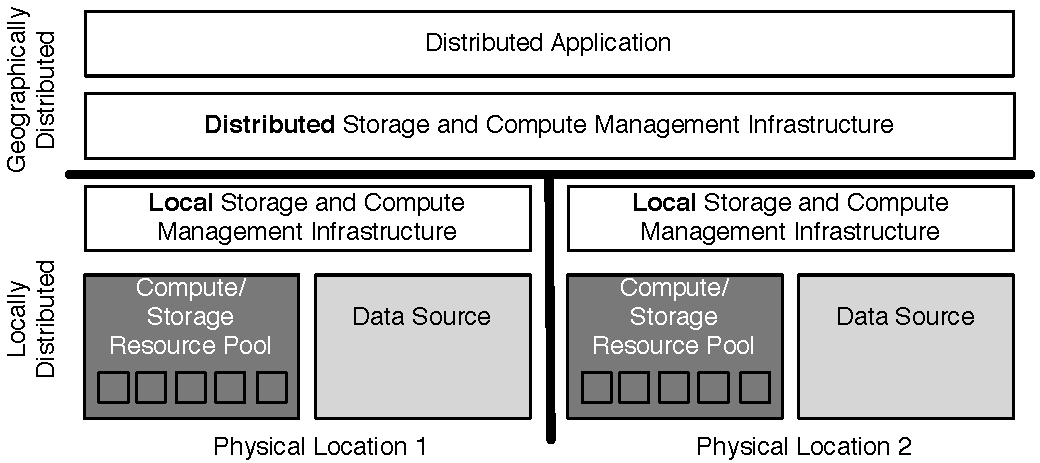
\includegraphics[width=0.7\textwidth]{figures/terminology.pdf}
%	\caption{Levels of Distribution}
%	\label{fig:figures_terminology}
%\end{figure}


% (\S\ref{sec:prog_infra}). \katznote{removed this ref, as it seemed
% out of place to have a ref to a subsection in the intro, as the only such ref}

% \subsection*{Distributed Data}
% One specific attribute that we believe is pervasive but not
% necessarily obvious is ``dynamic data.''  Additionally the requirement
% of many applications impose a requirement that data is dynamic.


% \jhanote{I do not know why floating sensors was a subsection? As an
%   examplar for D3 Science? If so, made it a subsubsection..}

%   \katznote{as I wrote in the title, it got moved from apps and won't be there
%   any more, but there was some thought that it might be useful as an example
%   application here.  Feel free to delete it if you don't think it adds anything here.}

% \subsubsection{Floating Sensors -- material than can be used in 1 as
%   an example application that is not going to be discussed in
%   \S\ref{sec:scenarios}}


% This {\em traditional application} constructs real-time hydrodynamics models, and forecasts the behavior of a complicated water system: the Sacramento
% - San Joaquin River delta.  It begins after data generation and includes data transformation \& decisions, storage, and processing.

% \subsubsection*{Application description}

% The application integrates both static and dynamic sensors streaming
% real-time data with a high-resolution hydrodynamics model running on
% the NERSC Magellan cloud testbed. The model uses sensor data to
% initialize and shape the run, and the model output is in turn used to
% drive the real-time positioning of the dynamic sensors. The output of
% this process is a map of the current and future behavior of the
% modeled watershed.

% Custom built dynamic sensors are deployed in the watershed along with
% traditional statically placed sensors that provide data. These sensors
% communicate over a variety of different network infrastructures, e.g.,
% GSM, CDMA, 802.11, wired ethernet, etc.  and the application acquires
% the data over the internet from the sensor platforms.  The application
% processes the sensor data in real-time as it is streamed.

% \subsubsection*{Big data aspects}

% Not known.

%  \subsubsection*{Distributed aspects}

% Not known.

%  \subsubsection*{Dynamic aspects}

% The sensor are all streaming real-time  data to the application. The position of the dynamic sensors
% themselves change over time.


%  \subsubsection*{Other important issues}

%  The first full, end-to-end, field test of the system is scheduled for
%  May 2011.

%\jhanote{If some one knows a bit more about Bayesian
%  approaches/inference/statistics and its 'implication' on dynamic
%  data via dymamic models, i'd love to hear / learn more}



%\katznote{some of this is repeating ideas from the para ``An important
%  motivation...''  Perhaps these two paras should be
%  combined?}\jhanote{DSK, this should not be an issue now, given that
%  this has now moved upstream}

%\jhanote{refine next four paragraph...} 

% Further, we define the degree as the number of data sources and sites that are
% used for storing and processing the data. A distributed application is an
% application that is composed of entities (i.e., either storage/compute resource
% or a data source) from at least two physical locations. In this work, our focus
% is almost exclusively on geographically distributed data and applications.


% Although the capacity to store data centrally is growing faster than Moore's
% Law, it is not sufficient in all cases to be able to ``dump the data'' in one
% place (or in the cloud.)  Oftentimes the costs (data transfer, storage,
% consequences of catastrophic failure) prevent the centralization of data, and
% decentralization---storing or place data in multiple locations---become prudent.

% Conversely, not all production of data is centralized; in some cases there are
% multiple producers (and consumers) of data, not to mention one-of-a-kind data
% that must be shared across multiple consumers.  Furthermore in collaborative
% science, data output from one analytical engine are often the input for the next
% stage of the analytical pipeline.  Last but not least, distribution via
% replication is a tested and effective approach to reliability and
% fault-tolerance; we will argue that it is also potentially a great performance
% enhancer and a means to ensure data consistency too.



\subsection{Scope}

% Before a discussion of the applications, infrastructure and research
% methodology, a brief mention of the motivation and thereby scope of
% this work is in order.

% Without a doubt, the era of {\it BigData} is here. However, BigData
% is not just an issue of large volumes of data, it is also about the

%One motivation of this work is to understand the complexity and
%characteristics of data that emerge as a consequence of scale, namely
%the dynamic properties and the distribution of applications, and the
%complex interplay between them that arises.

One motivation of this work is to understand the dynamic properties
and the distribution of applications, and the complex interplay
between them that arises as a consequence of scale.  Additionally, we
are motivated by an attempt to understand infrastructure---existing
capabilities, trends, and limitations---available to support the complexity,
challenges and characteristics of dynamic and distributed data at
scale.

We would like the reader to keep in mind some points regarding context and scope:

%\katznote{a lot of this paragraph seems too repetitive of the previous
%  section} \jhanote{Dan, I fixed the previous paragraph. OK?}

\begin{itemize}

\item This {\it survey} is not meant to be complete, either in the scope of domains
  covered or the types of infrastructure and application surveyed.  It
  represent the interests and experience of the authors. The specific
  requirements and barriers of applications cited in this paper are
  representative of the time at which the applications were surveyed
  (2012-2013); this is also true of the quantitative analysis of applications.
  
  % \katznote{need to add a note about the dates in which application data was
  %   collected?  I'm not sure the numbers are correct today, for example, from
  %   ATLAS}\jhanote{Fixed. CF ATLAS: I'll ask Kaushik/ATLAS to check}

\item The focus is generally on applications and infrastructure that arise from science
  and engineering projects in academia in general; this is a
  guiding principle.  While we are cognizant of enterprise applications and
  infrastructure, and recognize the impressive advances made therein, we also
  acknowledge that the factors such as scale, distribution, open-source, and
  interoperability influence the solutions employed and infrastructures used; it
  is important to therefore focus on problems that emerge in the space
  defined by these ``academic constraints''.

\item Almost by definition, any attempt to capture the state-of-the-art of such
  a dynamic and emerging domain is bound to be fraught with limitations and
  issues of scoping.  A complete and rigorous survey is bound to be obsolete by
  the time it emerges; so given the rate of change, we asked what could be
  done. What we present is a partial analysis motivated by a set of existing and
  active D3 applications, their trials and tribulations, successes and
  solutions. We believe there is merit in capturing the state-of-play as is,
  deriving a research agenda and set of specific yet crosscutting issues, and
  presenting these to the community.

\item Distribution can occur on many levels.  In this paper, we use {\em locally
    distributed} to indicate that data/compute resides on multiple nodes within
  one data center.  {\em Geographically distributed} describes the distribution
  of data and/or compute across multiple data centers.  Also, our focus is
  primarily on infrastructure considerations at  large scale, as searching
  for common solutions and patterns at  large scale is likely to be more
  fruitful than at small scales where customized tools and optimization of
  low-level systems features is likely to return greater yield.

  % Analogous to the distinction between programming in the large versus system
  % level programming, there is a distinction between the ``infrastructure''
  % considerations at the large-scale versus the small-scale.

\end{itemize}


%\jhanote{I think these two points can be ignored. To be discussed. But
%  either way this should go in the scope subsection}
%  \katznote{Dan and Shantenu request that Neil and Omer think
%  about the next two points, and either flesh them out with text
%  or remove them.}
%
%\begin{itemize}
%\item How does this differ from Scientific Databases? How does it
%  relate to Scientific Data Management and Scientific data flow
%\item Reference to EU 2030 Objectives (part of the Project Europe 2030
%  Report) -- underpins ``Data Intensive Research'' from an EU
%  perspective (strategy) + relate this to NSF ``CIF21'' vision
%\end{itemize}

%\jhanote{some points to ensure we've addressed. I cut and paste some
%  comments we received from the DPA survey paper that we should be
%  ensure at addressed -- implicitly or explicitly}
%
%\begin{verbatim}
%
%(i) It is difficult to argue about the completeness of the presented
%material.
%
%(ii) Picking a handful of distributed applications to study does not form a
%basis of a taxonomy.
%
%(iii) Furthermore, it is unclear if the applications
%are indeed representative of any urgent need to execute across
%distributed systems as the authors claim.
%
%(iv) At the same time, there is not enough description of the computer
%science behind the applications.
%
%(v) Several applications seem similar to each other and,
%as far as I can tell, do not add anything new.
%
%(v) The section is more a
%laundry list of applications - I would have expected to see a
%synthesis of different application and, for example, a classification
%into different classes. No general requirements of applications are
%derived. A smaller number of more representative sample applications
%(not covering nine pages) would have been better.
%
%(vi) My main problem with the paper is the research methodology.  The paper
%uses 6 hand-picked applications to derive a vector of attributes for
%each of them, derive some patterns from observing these vectors, and
%uses these patterns to perform a distributed computing tools gap
%analysis.
%
%(vii) It is unclear how important the applications used in this
%study are.
%
%(viii) Your lack of depth in explaining the applications leaves the
%reader empathetic.  It's important that the reader feels that they can
%learn something from reading this paper.  How is what you are saying
%applicable to me (a computer scientist or computational domain scientist)?
%
%(ix) Have you considered adopting a different approach, like conducting a
%survey to glean the likes/dislikes of distributed application
%developers?  In essence focus on the development process, as opposed
%to applications.  With a large enough pool of responses, you may come
%up with statistically significant conclusions that will be of interest
%to the wider community.
%
%\end{verbatim}



\subsection{Outline of this paper}

The remainder of this paper consists of
the application scenarios (\S\ref{sec:scenarios}),
a discussion of the aspects of distribution and dynamism in the
applications (\S\ref{sec:distdyndata}),
a description of the software infrastructure required for D3 applications
% Yogesh: This section's description seemed more verbose than others, hence commenting out details
% , such as
% software frameworks, tools, and middleware and platform services
(\S\ref{sec:infrastructure}),
analysis and characterization of the applications and
conclusions (\S\ref{sec:conclusions}).

\section{D3 Application Scenarios \label{sec:scenarios}}

Starting with the experience of the attendees of the 3DPAS workshops,
we have assembled a set of D3 ``applications'' that we describe in
this section.  We realize that we have overloaded the term application
here.  In this document, some of our applications are really {\em
  traditional applications}, meaning a program that is developed by a
user or project to try to answer a science question, usually with some
input data needed and some output data produced.  Applications in this
category are: NGS Analytics (\S\ref{bioSilvia}), CMB
(\S\ref{astroJulian}), Fusion (\S\ref{fusionScott}), Industrial
Incident Notification and Response (\S\ref{Kees}), MODIS Data
Processing (\S\ref{modisKeith}), and Distributed Network Intrusion
Detection (\S\ref{detectionJon}).

Another group of applications are {\em infrastructural applications}.
Applications of this type are collaborative, in that they depend on a
context that is often agreed upon by a community, most often in terms
of how data is stored by the community and how it is accessed, as well
as, more often than not, a weak consensus on the infrastructure to be
used. %\jhanote{Dan: Please confirm you are OK with this modified
%  defintion of infrastructural application}
This allows different
sub-applications (that we again refer to as `applications') to focus
on different stages, such as generating data, or processing data.
Answering a science question now may involve a set of applications
that need to be run in series, perhaps in different stages, that may
be run by different groups that do not frequently interact.  This type
of application includes: ATLAS/WLCG (\S\ref{WLCGSteve}), LSST
(\S\ref{astroAdam}), SOA Astronomy (\S\ref{astroSOAAdam}), Sensor
Network Application (\S\ref{sensorSimon}), Climate
(\S\ref{climateDan}), Interactive Exploration of Environmental Data
(\S\ref{envJon}), and Power Grids (\S\ref{power}).

In other words, multiple infrastructural applications are used together in particular
science domains.  Furthermore, infrastructural
applications involve more than just the end user (scientist), and
typically require exerting control at layers below, i.e.,
``programming the system (infrastructure)'', as opposed to a
traditional applications, where end user effort and control is often
confined to a well-defined application kernel.


% \jhanote{Need better distinction between infrastructure and
%   traditional applications. They are the same at the scale-up and
%   scale-out level, but different in scale-across and people. Another
%   issue is that about ``control and configure'', i.e traditional
%   applications only exert control and configure the application layer,
%   whilst infrastructure applications need to configure the lower
%   ie. infrastructural layer too}

% \katznote{I don't agree in general that more is needed, but if you
%   think so, please give it a try.  I also don't agree specifically
%   that infrastructure applications `configure' the lower layer.
%   Rather, I would say they assume a particular, community-defined
%   (perhaps de facto) layer.  Finally, while I understand scale-up
%   and scale-out, and I don't know what `scale-across' is.}

Some of the applications we describe are really groups of
applications, meaning that we are grouping together a number of
independent programs, written by different authors, that are trying to
answer the same type of science question, where a single user
will only run one of them at a time.  %\katznote{Shantenu, please check
%the preceding and see if this is ok, in the context of the whole
%paragraph and section.}
These codes and their developers may either be
competing or collaborating, and sometimes both, informally known as
collabetition. Specifically, this is the case for NGS Analytics
(\S\ref{bioSilvia}), SOA Astronomy (\S\ref{astroSOAAdam}), and
Interactive Exploration of Environmental Data (\S\ref{envJon}).  (Note
that this issue is orthogonal to traditional vs. infrastructural applications:
NGS Analytics is traditional, where SOA Astronomy and Interactive
Exploration of Environmental Data are infrastructural.)  In
each of these examples, we have chosen one specific application that
is meant to represent a possibly large number of comparable
applications.

%\jhanote{Dan: This paragraph seems to suggest some
%  similarity with infrastructural applications, but doesn't quite do
%  so. Can we make a bit more explicit the intent. For example, If we
%  break into ``collaborating'' vs ``competing'' and put NGS into a
%  ``competing'' category the remainder of the paragraph above would be
%  a useful and fair elaboration on infrastructural applications?
%  Reading forward, Section 5.1, it appears to be consistent with the
%  ``observations'' section. For example, `` Some of the applications
%  we describe are really groups of applications, meaning that we are
%  grouping together a number of independent programs, written by
%  different authors.  These independent programs might be competing
%  means to answer the same type of science question and thus are not
%  intended to run together, or they could be a set of smaller
%  applications collaborating to answer the same overall science
%  question.''}  \katznote{some changes made above.  I'm not sure why
%  NGS is competition and the others are collaboration - to me they are
%  all a bit of both.} \jhanote{NGS is classified as a traditional
%  application; others as infrastructural and as having multiple
%  distinct applications. Thus it is natural to have collaborative.
%  But as NGS is said to be a traditional, different applications can
%  be perceived to be competitive. I agree that the term competitive is
%  not perfect} \katznote{I've added a note to say that this (applications
%  selected to represent groups) is orthogonal to traditional vs
%  infrastructural.  (This is actually why this is a different paragraph.)
%  Does this help?}


%\katznote{not sure which category is right for: Power
%Grids (\S\ref{power})  Yogesh, what do you think?}
%\ysnote{The infra category is appropriate. i.e. no change required}

%\alnote{After reading the definition a couple of times, I still have a
%difficult time to distinguish between infrastructural and archetypical
%applications. The definitions sound very similar.}
%\katznote{this section has been re-written.  I've removed archetypical applications, and added a paragraph at the end of this section (2.0) to mention this idea without naming it.  Please see if this is now better.}
%\alnote{reads very well!}

The discussions in the workshops and our analysis of the applications
led us to examine the use of data in different parts of the
applications, where we found some common patterns
across applications.  For example, applications that involve
streaming data collect data from sensors, transform and
filter the data, store the results, and then later process (analyze)
the stored results.  In general, we think that all of the applications
we have studied can be mapped to a set of stages or phases.  This is
illustrated in \figurename~\ref{fig:figures_application-stages}.

The question of where the application, as opposed to the entire
system, %(where the system is defined as all of \figurename~\ref{fig:figures_terminology}), 
actually starts
is somewhat difficult.  In this paper, we have decided not to treat
hardware data sources (e.g., sensors, telescopes) as part of the
applications.  Therefore, these applications generally start with the
data movement that follows the actual data generation.

Unlike the sensor applications, another set of applications generate
data computationally, for example, from a model or simulation.  These
applications then do start with data generation, and they often have
just three stages, where data is generated in the first stage, stored
in a second stage, and then processed in a third stage (i.e., the
transformation \& decisions stage in
\figurename~\ref{fig:figures_application-stages} does not occur).

Other
applications may operate on stored data (i.e., they only contain the
processing stage and its associate data movement).
%\alnote{We should refer to these application stages from the
%  application descriptions. Currently, this classification is not
%  used.}  \katznote{have now done, but this was harder to do than I
%  thought it would be, particularly to define where the application
%  starts - for example, LSST as an app does not include data
%  generation, but starts after this (data transformation \&
%  decisions), and SOA Astronomy does not include data storage, but
%  does include the movement from the storage.  Perhaps I need to go
%  back and make the fact that many apps start with data movement more
%  clear.}\alnote{ok}

\begin{figure}[htbp]
    \centering
        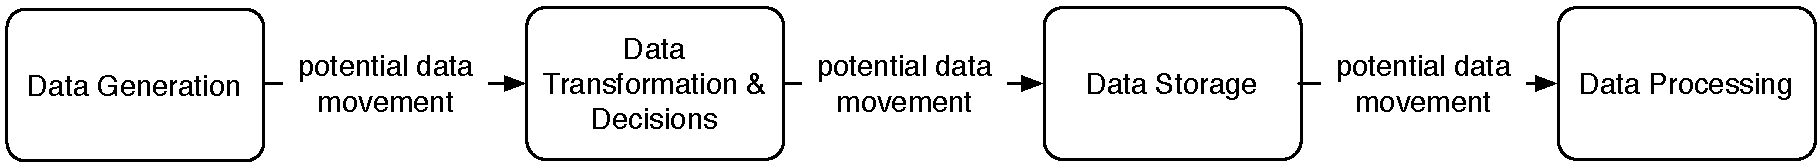
\includegraphics[width=1.0\textwidth]{figures/application-stages-new.pdf}
        \caption{Application Stages: The work in data-intensive
        applications can be put into four common application stages:
		data generation, transformation \& decisions, storage, and processing, though not all
		applications have all stages.
%		\alnote{We have some applications (e.g. sensor networks) that give feedback to the
%		data generation stage. Do we want to refer to this possibility here?}
%		\alnote{data transformation and decision making sounds to me similar to processing}
%		\katznote{what do you suggest?}\alnote{The proposal would be to just call it Data Processing as before. Since
%		 there are many forms of processing (transformation being just a specific form of processing)} \katznote{I want to distinguish between the processing that happens before storage
%		 and the processing that happens after storage, so I am thinking of not changing this.
%		 Would this really bother you?}
                \label{fig:figures_application-stages}}
\end{figure}


%\katznote{Dan to clean up the description of app phases in the intro and the apps,
%explain where apps start, with data movement, data generation, data storage, etc. --
%then ask Shantenu to read and comment on this.}

%\katznote{think about linking this with 4.1}

%Application Scenario Characteristics for Dynamic Data (Various)
%
%Identify: (1) what is the case scenario within the application; (2) what data is dynamic; (3)  how the data is being used in the context of each of these scenarios.
%
%\katznote{proposed structure for rewriting these entries:\\
%1. what does the application do - what problem does it solve (question 1 below) \\
%2. how does it do it (questions 2,3,5,6 below, also address cyberinfrastructure (where does the app run)) -- perhaps have a diagram here of what happens in the app \\
%3. what are the big data aspects (question 4b below) \\
%4. what are the distributed aspects (question 3 below)\\
%5. what are the dynamic aspects (question 4a below)\\
%6. what else is important (questions 7,8 below, also address programming systems (how was the app written; what tools does it use))\\
%}
%
%
%Currently trying to do this by asking the following questions:
%\begin{enumerate}
%\item[1] What is the purpose of the application?
%\item[2] How is the application used to do this?
%\item[3] What infrastructure is used? (including compute, data, network, instruments, etc.)
%\item[4] What dynamic data is used in the application?
%\begin{enumerate}
%\item[4a] What are the types of data,
%\item[4b] What is the size of the data set(s)?
%\end{enumerate}
%\item[5] How does the application get the data?
%\item[6] What are the time (or quality) constraints on the application?
%\item[7] How much diverse data integration is involved?
%\item[8] How diverse is the data?
%\end{enumerate}
%
%Please feel free to also talk about the current state of the
%application, if it exists today, and any specific gaps that you know
%need to be overcome.

%\subsection{Silvia's Biosciences app: NGS, medical imaging (Silvia)\label{bioSilvia}}

\subsection{Next Generation Sequencing (NGS) Analytics \label{bioSilvia}}

The (grand) challenge in bioinformatics is the need to provide support
for the analysis of genome sequence data that is becoming available
due to the abundance and high-throughput capability of the
next-generation sequencing devices. The rate of growth of data from
the NGS machines humbles Moore's law; it has increased by more than
three orders of magnitude in barely a decade.

There are many different types and components of analyses of NGS data.
However, fundamentally important to all types is the ability to
efficiently and effectively map/align the short reads to a reference
genome.

Alignment underpins multiple scientific questions such as comparing
metagenomic (DNA sequence) data sets against each other, which could
be used to distinguish human disease biomarkers among different
individuals, determine different soil (or water or air or ...)
microbial composition from different samples, etc.

This subsection describes a set of {\em traditional applications} that
are used in the processing of next generation sequencing data.  The
applications have two of the possible stages: data storage and data
processing.
%\katznote{Shantenu/Yogesh, can you confirm this or fix it?
%  I'm sure data generation is not part of this app, but am not sure
%  about transformation \& decisions. - see
%  Figure~\ref{fig:figures_application-stages}.} \jhanote{Dan: I'm
%  confused. Not sure I understand what you mean by data-generation is
%  not part of this app?}
%  \katznote{the sequencer is not part of the application - the application
%  starts once the data has been generated, thus it starts on a data movement
%  arrow.  I'm just not sure which one.}\alnote{I think the phases storage and
%  processing are fine for NGS}

\subsubsection*{Application description}


There are multiple tools (programs) that can perform the mapping/alignment
phase, e.g., BWA, BFAST, Bowtie, MAQ, etc. Each has its own strength and
its own native data support/capability; they also implement
different alignment algorithms. Thus, based upon different design
objectives and trade-offs, they typically have different constraints
and efficiencies.

Several of these tools are also composed together as a linear pipeline
for performing sequencing and analysis. The pipeline may go through
alignment, SNP calling, haplotyping, and so on, with different tools
used in each stage. These pipelines can often be performed
independently on each chromosome to provide simple parallelism.

All algorithms, architectures, storage, and networks have broken or
will break soon.  Some NGS analytics are not good fits for core-rich
and memory-poor modern architectures. Some problems (e.g., comparing
k-mers across metagenomic data sets) need terabyte-scale memory, not
thousands of cores.~\cite{ngs-gap}

Individual data sets, which will be terabyte-scale, are generated by
NGS machines at a variety of locations. There could be many thousands
of such sets to compare. Having them all local may not be feasible
(the transfer time from where they are generated may be prohibitive).

\subsubsection*{Big data aspects}

Individual data sets will be terabyte-scale. For example, for a
standard genomic sequence, there are billions of short (35-100 bases)
reads of DNA.  And there could be many thousands of such sets to
compare for a given problem.  Getting more accuracy for sequencing may
require multiple coverage (e.g. 10x), that can cause sequence sizes to
increase linearly.  This makes NGS data management fundamentally a big
data problem.  NGS analytics, in addition to being a big data problem,
is also a computationally demanding and distributed computing problem.
The computational demands arise from the often complex and intensive
analysis that has to be performed on data, which in turn arise from
algorithms that are designed to account for repetitions, errors and
incomplete information.

\subsubsection*{Distributed aspects}

The type of NGS research being conducted can distinguish the
distributed properties of the application. Researcher groups that
own sequencing machines need to deal with large dataset sizes that
need to be re-sequenced and reduced for further analysis. Other
researchers may analyze large catalogs of sequenced genome databases
are maintained, and perform pattern matching. Further, clinical may be
interested in in-depth analysis of an individual sequence for disease
diagnosis or visualization.

The distributed computing aspects arise at multiple levels: for
example, the simple act of having to move data from source
(generation) to the destination where computing (analysis) will occur
is a challenge due to the large volumes involved. Trade-offs exists
between the cost/challenges in distributing data versus I/O
saturation or memory bottlenecks.

When coupled with the compute intensive nature of the problem, it soon
emerges that a fundamental challenge is not only whether to
distribute, but where to distribute, what to distribute (should the
computing move to the data, or the data move to the compute), and how
to distribute (what tools and infrastructure to use).

\subsubsection*{Dynamic aspects}

The dynamic challenges of NGS data are more subtle; the data
themselves are not dynamic -- the sequences are acquired once and
analyzed many times. However the execution of these applications on
distributed infrastructure have dynamic aspects when optimized
resource usage is considered. For example, workload decomposition and
distribution must be determined dynamically in order to optimally use
resources, e.g., compute resource selection can be based on data
location, processing profile and/or network capacity.

\subsubsection*{Other important issues}

There are several toolkits that have emerged for NGS providing
incrementally better algorithms for sequencing and analysis
\cite{SAMtools, BioJava, BioPerl, .NETBio}.  However, as a consequence
of the broad range of infrastructural requirements, there isn't
currently a common ``standard'' cyberinfrastructure used for NGS
analytics; researchers use what is easily available to them, or try to
use COTS infrastructure. Historically, leaders in the field have
developed infrastructure for the larger community to build-upon, e.g.,
QCDOC or MD-GRAPE. But given the broad range of requirements, a
hardware-only solution is unlikely for a broad range of problem
instances, and a combination of hardware and software approaches will
be employed. This reinforces the need for flexible programming systems
and associated run-time environments that support collective
(hardware-software) optimization.

%\alnote{What kind of codes are used
%in these clusters? What are the characteristics of these codes?}
%But any additional analysis is not supported.
%\alnote{What would be an additional analysis}
%

NGS sequencers such Illumina and Ion Torrent provide the option of onsite
servers or small clusters for performing the alignment and re-sequencing as a
pipeline right after the reads have been generated.  Scientific workflow systems
like Taverna~\cite{Taverna:2006}, BioKepler~\cite{biokepler:2011}, and
Galaxy~\cite{galaxy} (though Galaxy does not support distributed systems
currently) have been successful in integrating genome analysis tools for
bioinformatics. Script-based pipelines that combine executables are also often
used. Very few workflow systems have explicit support for distributed data or
dynamic data handling.  Therefore reusable approaches at extending existing
tools to support distributed and dynamic data are likely to be useful.
%\katznote{Shantenu/Yogesh/Andre, please read this paragraph and tell me if changes
%should be made to this section at this point}\alnote{ok with me}

%\alnote{Some details on how distributed/dynamic data is handled in
%  these workflows would be good.}

%\katznote{from Silvia Delgado Olabarriaga, Tom Slezak, and Shantenu}
%
%\katznote{summary below assigned to Shantenu}

%\subsubsection{new summary}

%\katznote{Please make a new title for this section}

% \katznote{I was assuming you would leave the questions here, so that
%   we could pull some of this material into a table later...}


% 1. {\bf What does the application do? What problem does it solve?}

% \katznote{from answer to question 1}

%2. {\bf How does it do it?}

% \katznote{from answers to questions 2,3,5,6
%   below, also address cyberinfrastructure (where does the app run) --
%   perhaps have a diagram here of what happens in the app}

%\ysnote{The first para of this section reads more like ``what does the application do'' rather than
%  ``how''. Should it move above? Also, the description of cores/memory above can move here as it
%  relates to CI. }
%\ysnote{This section will benefit from describing the (often) linear pipeline of
%  sequencing, with individual chromosomes that can be processed independently.}
%\katznote{Yogesh or Shantenu, can you do address Andre's comments in this section?}
%\ysnote{I've taken a pass. Shantenu, do you care to make changes?}
% 3. {\bf What are the big data aspects?}  \katznote{from answer to
%   question 4b below} 4. {\bf What are the distributed aspects?}
% \katznote{from answer to question 3 below} \ysnote{distinguish
%   between individual research project where compute can move to
%   data; clinical testlabs that sequence and transmit sequenced data
%   to end user for post processing; collaboratory projects like
%   1000-genome where data has to be aggregated centrally. Sequencing
%   done remotely but visualization done locally.}
%5. {\bf What are the dynamic aspects?}
%\katznote{from answer to question 4a below}
%6. {\bf What else is important?}

%\katznote{from answers to questions
%  7,8 below, also address programming systems (how was the app
%  written; what tools does it use)}

%\ysnote{See biohpc.net, bioperl, biojava, bio.net}
%\katznote{I'm not sure what action goes with this comment.  Yogesh?}
% It is unlikely that researchers or NGS teams will build integrated
% customised infrastructure for no cyberinfrastructure to solve this
% problem. The solution to

% \katznote{do we want to retain the figure? - currently commented out}


% In general this is a large (for biology -- don't think in terms of
% exascale!) data problem with large (all-vs-all comparison)
% computing. There are strategies to make this more scalable that will
% reduce the computing volume.

% i) large (exascale) data and large (exascale) computing (e.g., data
% mining, analytics, bioinformatics)

% ii) large (exascale) data and modest computing (e.g., search)

% iii) modest data and large (exascale) computing (e.g.,
% simulation/modeling)

% Potentially peta-bytes or exa-bytes of data. Not sure how to quantify
% the computing. (Huge memories will be potentially more valuable than
% huge numbers of cores -- although this is heresy to the physics
% crowd.)

% Computing might then have to be
% distributed. Biology is wrestling with this now.


% Although only the alignment step is computation-intensive, it is
% more practical to perform all the others on the grid to minimize data
% transport to/from the user's workstation, which is normally on low
% speed networks. That is, the computation is statically and manually
% taken to the data in this case. This can lead to sub-optimal resource
% usage.

% Data is not really `dynamic' in this case -- the sequences are
% acquired once and analyzed many times. However the execution of this
% application on a distributed infrastructure has dynamic aspects when
% optimized resource usage is considered:

%\begin{itemize}
%\item Split/merge the data according to available resources
%\item Compute resource selection based on data location, processing profile and/or network capacity
%\item Resource selection based on security constraints (access control, trust)
%\item Collection and processing of monitoring information to steer grid enactment.
%\end{itemize}
%
%
%\subsubsection{old material follows}
%
%\begin{itemize}
%\item Infrastructure monitoring for the execution of workflows to
%  manage failure
%\item the application is sequence alignment (split data (this is where there is dynamic decision making) to execute the alignment in parallel)
%\item DTI Imaging: two cases are interesting: DTI atlas (split, run, merge, split, merge - reduction from 10000 tasks to 1 output); PCA for classification of patients/control
%\end{itemize}
%
%\subsubsection{Silvia's contribution}
%
%NGS sequence alignment on the AMC e-bioscience infrastructure
%
%1. What is the purpose of the application?
%
%The application performs analysis of DNA sequencing data for various
%goals in life science research, e.g., Mutation screening, Virus
%discovery, Genome-wide Associations (GWA), Linkage analysis,
%Comparison of bacterial genomes, microRNA expression and Exome
%sequencing. The data analysis is composed of various methods that are
%implemented by a bioinformatician, whereas the data is typically owned
%by the life scientist.
%
%2. How is the application used to do this?
%
%Note: Here we focus on data analysis from the perspective of the
%bioinformatician, excluding steps related to data acquisition
%(transformation of raw images into sequences of amino acids) and
%posterior biostatistics and epidemiological analysis.
%
%The data analysis is implemented as a pipeline of generic and
%customized components, mostly third-party public software tools. The
%pipeline may differ for each specific study, depending on the data
%acquisition and the research question. Typically it includes data
%preparation (file conversion, reformatting and filtering); alignment
%(comparison) with some reference database as the human genome;
%post-processing (output conversion, reformatting, statistical
%analysis) and visualization. Sequence alignment is the most
%computing-intensive step, which became prohibitive for sequential
%execution in next generation sequence experiments. All data is stored
%in files that are often completely read in memory for fast
%processing. Compressed formats are usually adopted. Although the files
%are large, the data can be easily decomposed because the processing is
%done on each sequence (`string') at a time.
%
%3. What infrastructure is used? (including compute, data, network,
%instruments, etc.)
%
%\begin{figure*}[htbp]
%  \begin{center}
%    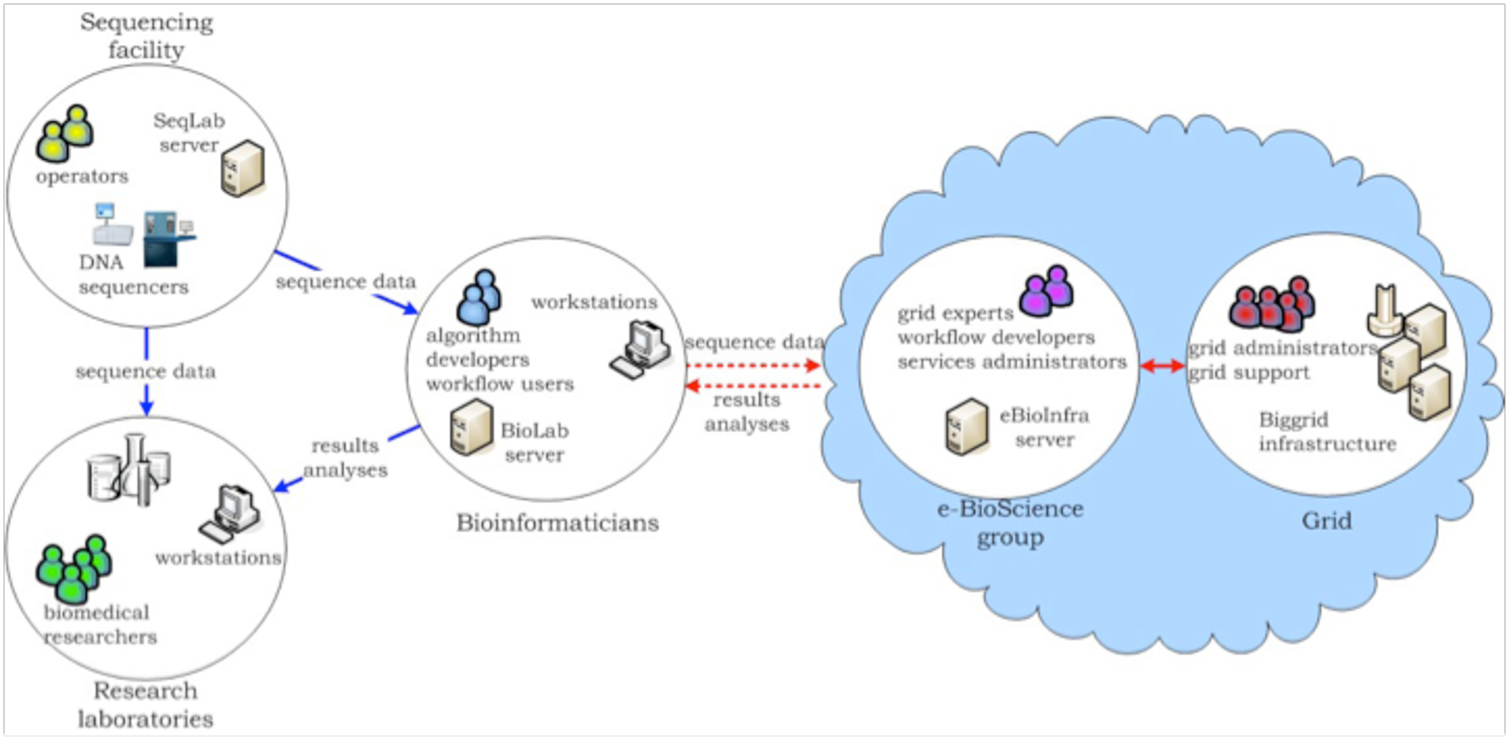
\includegraphics[width=\textwidth]{figures/silvia.pdf}
%    \caption{Figure from Silvia}
%    \label{Fig:silvia}
%  \end{center}
%\end{figure*}
%
%see Figure~\ref{Fig:silvia}.
%
%Data:
%
%Data acquisition: Roche, Solid and Illumina next generation sequencers
%
%Local storage: dedicated server at the AMC network (ftp)
%
%Grid storage: Storage Elements of the Dutch e-Science Grid
%(www.biggrid.nl)
%
%Data transport:
%
%From sequencer to server: AMC network (XXX) or off-line media
%
%Between data server and grid storage: public network (XXX); lightpath
%(near future)
%
%Between grid storage and worker nodes: public (XXX) or site (XXX)
%network
%
%Computing:
%
%Local Computing: clusters and servers at the AMC and workstations
%(laptops, desktops) anywhere Grid Computing: Dutch Grid
%(www.biggrid.nl), part of EGI
%
%Originally all steps were performed in some local server or on the
%user's workstation. The visualization is still performed in the user's
%(windows) workstation, but all the other steps are currently performed
%on the Dutch grid infrastructure. The pipeline is described as a grid
%workflow using the GWENDIA language
%(\url{http://dx.doi.org/10.1145/1645164.1645171}) and enacted on the
%Dutch Grid using the MOTEUR2 workflow engine
%(\url{http://modalis.polytech.unice.fr/softwares/moteur/start}).
%
%PS: although only the alignment step is computation-intensive, it is
%more practical to perform all the others on the grid to minimize data
%transport to/from the user's workstation, which is normally on low
%speed networks. That is, the computation is statically and manually
%taken to the data in this case. This can lead to sub-optimal resource
%usage.
%
%4. What dynamic data is used in the application?
%
%Note: data is not really `dynamic' in this case -- the sequences are
%acquired once and analyzed many times. However the execution of this
%application on a distributed infrastructure has dynamic aspects when
%optimized resource usage is considered:
%
%\begin{itemize}
%\item Split/merge the data according to available resources
%\item Compute resource selection based on data location, processing profile and/or network capacity
%\item Resource selection based on security constraints (access control, trust)
%\item Collection and processing of monitoring information to steer grid enactment.
%\end{itemize}
%
%(a) What are the types of data,
%
%DNA sequences (strings) stored in open formats (FASTA, SFF, SAM, BAM)
%Bundles of results from alignment tools (custom format, binary?)
%
%(b) What is the size of the data set(s)?
%
%one example for BWA alignment tool (short sequences) follows:
%
%input data: Sequencing Data in the csFasta format, normally 25-35~GB;
%Quality files in the .qual format, normally 50-80~GB; Reference DB in
%the Fasta BS format: 3.2~GB (human genome) 140~MB (one chromosome)
%
%Intermediate files: Reference BWA index, normally 4.5GB (human genome)
%240~MB (one chromosome); Sequencing Data in the FastQ format
%(fastq.gz), normally 20-30~GB
%
%Output: Results in .sai format (direct output of BWA), normally
%2-3~GB; Results in .sam format, normally 55-75~GB; Results in .bam
%format, normally 20-30~GB
%
%5. How does the application get the data?
%
%From a local file. The legacy code is wrapped to stage the inputs and
%outputs in/out the worker node.
%
%All data is stored in files that are often completely read in memory
%for fast processing. Compressed formats are usually adopted. Although
%the files are large, the data can be easily decomposed because the
%processing is done on each sequence (`string') at a time
%
%6. What are the time (or quality) constraints on the application?
%
%In research there are no strict constraints on the time to complete
%the analysis.  In patient care, time could determine life, death or
%money, but we have no concrete case yet.
%
%Quality in this case refers to the accuracy of the results
%obtained. This is essential for research and patient care.

\subsection{ATLAS (an Example of Use of the WLCG) \label{WLCGSteve}}

%\katznote{from Steve Fisher}
%
%\katznote{summary below assigned to Dan}
%\subsubsection{new summary}

%1. {\bf What does the application do? What problem does it solve?}

%\katznote{from answer to question 1}

The Large Hadron Collider (LHC)~\cite{lhc} at CERN in Geneva is
producing a large amount of data across a number of experiments,
including ATLAS~\cite{atlas}. The application discussed in this
section is an {\em infrastructural application} (meaning that it
consists of multiple stages that are run by different people, in this
case data acquisition, storage, distribution, and analysis). It has
the goal of allowing a physics group or a user to analyze data to
understand a specific physics channel (underlying physical process) as
recorded by ATLAS.  The set of available data grows steadily over time
as more data are collected (by the experiment) and reconstructed. This
application thus contains two stages: data storage and data
processing.
%\alnote{prev. also acquisition was
%part of the application} \katznote{I don't see that it should be.  Doesn't the app
%start after the data is in the Tier 1 archive?}

\subsubsection*{Application description}
%2. {\bf How does it do it?}

%\katznote{from answers to questions 2,3,5,6 below, also address cyberinfrastructure (where does the app run) -- perhaps have a diagram here of what happens in the app}

Both physics groups and individuals run jobs on the WLCG (Worldwide LHC Computing Grid)~\cite{lhcb} as they see fit, either reading the reconstructed data or reading intermediate datasets created by themselves or their colleagues. If, in the future, resources should prove inadequate then adjustments to working practices to coordinate processing may be made to increase physics output.

The WLCG has a hierarchical architecture. CERN (the `Tier~0' site) is connected to eleven `Tier~1' (national) sites by a dedicated optical network. This may be extended in the future.  All data is stored at CERN, and as needed, various parts of the dataset are copied (and cached, i.e., replicated) to the Tier~1 sites, and from there to `Tier 2' (regional) sites and to `Tier~3' (university or group or individual) sites.

Before data is analyzed, the file to be analyzed is copied from the closest site to the SE (Storage Element) at the WLCG site where the job will run. From there it is either copied to a local disk or read from the SE.

There is no particular time constraint on the processing, although physics groups are eager to understand the ATLAS experiments and thus want to process data as quickly as possible.  In the event some data are missed during processing, the only effect is a reduction of statistical precision in the final analysis. Accurate bookkeeping is therefore important in order to know which data have been processed.

 \subsubsection*{Big data aspects}
%3. {\bf What are the big data aspects?}

%\katznote{from answer to question 4b below}

Roughly 20~TB of data are collected every day. Multiple generations of processed data are kept. Many data files are replicated on multiple sites; this is done both by copying it to where it is likely to be useful and partly dynamically as the need arises.  The bulk of the data is individual event data at different stages of refinement. This is held in an in-house representation of C++ serialized objects. Though this format is not standard it is used by all LHC experiments.

 \subsubsection*{Distributed aspects}
 %4. {\bf What are the distributed aspects?}


%\katznote{from answer to question 3 below}

The WLCG has 250,000 cores distributed over 140 sites and with 100~PB of disk. It uses a mixture of gLite software, experiment specific software and physics group specific software.  The data is distributed and replicated as described previously.

 \subsubsection*{Dynamic aspects}
%5. {\bf What are the dynamic aspects?}


%\katznote{from answer to question 4a below}

The data being processed can be considered as dynamic as it grows steadily as new raw data are collected and the basic processing program (called reconstruction) is run to produce information about specific particles involved in a collision. This reconstruction is rerun periodically (two or three times per year is expected) as calibrations of the detector are improved. Reconstruction algorithms are also improved as are the physics groups' selection codes.
%\alnote{Is the reconstruction code the fundamental entity that is required to deal with new data? Sounds rather like an auxiliary tool.}
%\katznote{reconstruction is a second type of processing.}\alnote{should we explicitly state that?}

 \subsubsection*{Other important issues}
%6. {\bf What else is important?}


%\katznote{from answers to questions 7,8 below, also address programming systems (how was the app written; what tools does it use)}

Data analysis is really a pleasingly parallel task, where various events are analyzed in parallel and then a summary is created of all the analyses.

The key challenge here is really in the infrastructure -- building a system that can store massive amounts of data and move them to where the processing is to be done by a large diverse group of users.



%\subsubsection{old material follows}
%
%
%\begin{itemize}
%\item Most of the dynamism is in infrastructure, not in the application (e.g. use of PilotJob)
%\item Application dynamism: location of file (e.g. if file turns out to be not local, look up in registry-- but not do this again)
%\item No specific QoS issue concerned with data transfer times
%\end{itemize}
%
%\subsubsection{New answers from Steve}
%
%3DPAS - Particle Physics - the example of Atlas physics channel selection.
%
%   1.     What is the purpose of the application?
%
%A physics group is interested in a specific physics channel (underlying physical process) as recorded by the Atlas experiment at the LHC (Large Hadron Collider) at CERN in Geneva. The set of available data grows steadily over time as more data are collected and reconstructed.
%
%   2.    How is the application used to do this?
%
% Both physics groups and individuals run jobs as they see fit, either reading the reconstructed data or reading intermediate datasets created by themselves or their colleagues. If, in the future, resources should prove inadequate then adjustments to working practices to coordinate processing may be made to increase physics output.
%
%   3.      What infrastructure is used? (including compute, data, network, instruments, etc.)
%
%The WLCG (Worldwide LHC (Large Hadron Collider) Computing Grid) is used with a mixture of gLite software, experiment specific software and physics group specific software. WLCG has 250,000 cores distributed over 140 sites and with 100~PB of disk. CERN is connected to the eleven `Tier 1' national sites by a dedicated optical network. This may be extended in the future.
%
%   4.      What dynamic data is used in the application?
%
%The data being processed can be considered as dynamic as it grows steadily as new raw data are collected and the basic reconstruction program is run to produce information about specific particles involved in a collision. This reconstruction is rerun periodically (two or three times per year is expected) as calibrations of the detector are improved. Reconstruction algorithms are also improved as are the physics groups' selection codes. One output of the reconstruction is `tag' data - summary information written to a database to facilitate event selection. This is not yet used very much. Calibration data are held on an RDBMS with Frontier/Squid front ends.
%
%         a.             What are the types of data,
%
%          The bulk of the data is individual event data at different stages of refinement. This is held in a in-house representation of C++ serialized objects. Though this format is not standard it is used by all LHC experiments.
%
%         b.            What is the size of the data set(s)?
%
%          Roughly 20~TB of data are collected every day. Multiple generations of processed data are kept. Many data files are replicated on multiple sites; this is done both by copying it to where it is likely to be useful and partly dynamically as the need arises.
%
%   5.      How does the application get the data?
%
%A copy of the file is made to the SE (Storage Element) at the site where the job will run. From there it is either copied to a local disk or read from the SE.
%
%   6.      What are the time (or quality) constraints on the application?
%
%If some data are missed during processing the only effect is a reduction of statistical precision in the final analysis. Accurate book keeping is important to know which data have been processed. If the selection code has been improved then naturally the physics groups would like to see the results as soon as possible.
%
%
%\subsubsection{Old answers from Steve}
%
%   1.       What is the purpose of the application?
%
%A physics group is interested in a specific physics channel (underlying physical process) as recorded by the Atlas experiment at the LHC (Large Hadron Collider) at CERN in Geneva. The set of available data grows steadily over time as more data are collected and reconstructed. It would not be efficient to allow individual physics groups to process this large volume of data in an uncoordinated manner as it requires reading all available data.
%
%   2.       How is the application used to do this?
%
%Physics groups register their analysis code to be run on the next scheduled analysis ``train''. The train leaves every two weeks and reads through all the data, runs the physics selection code of each group and writes out the selected events and output from the computation to produce relatively small data sets for each physics group. The groups then use these selections to perform more ad-hoc analysis.
%
%   3.      What infrastructure is used? (including compute, data, network, instruments, etc.)
%
%The WLCG (Worldwide LHC (Large Hadron Collider) Computing Grid) is used with a mixture of gLite software, experiment specific software and physics group specific software. WLCG has 250,000 cores distributed over 140 sites and with 100~PB of disk. There is no wide area dedicated network infrastructure.
%
%   4.      What dynamic data is used in the application?
%
%The data being processed can be considered as dynamic as it grows steadily as new raw data are collected and the basic reconstruction program is run to produce information about specific particles involved in a collision. This reconstruction is rerun periodically (two or three times per year is expected) as calibrations of the detector are improved. Reconstruction algorithms are also improved as are the physics groups' selection code. Calibration data are held on an RDBMS with Frontier/Squid front ends.
%
%         a           What are the types of data,
%
%          The bulk of the data is individual event data at different stages of refinement. The is held in a non-standard representation of C++ serialized objects.
%
%         b.             What is the size of the data set(s)?
%
%          Currently the reconstructed data (excluding copies) is about m TB and is growing at about  n TB per month. Many data files are replicated on multiple sites. This is done both by copying it to where it is likely to be useful and partly dynamically as the need arises.
%
%   5.       How does the application get the data?
%
%This is mostly by copying the file to where the job will run - though some remote file access is also used.
%
%   6.  What are the time (or quality) constraints on the application?
%
%If some data are missed during processing the only effect is a reduction of statistical precision in the final analysis. If the selection code has been improved then naturally the physics groups would like to see the results as soon as possible.


%\subsection{Astrophysics -- Virtual Observatory (Bob) \label{astroBob}}
%
%\katznote{this will be merged into the LSST and SOA entries}
%
%
%\begin{itemize}
%\item Analysis of data to generate event streams $\rightarrow$ lead to the
%  positioning of telescopes
%\end{itemize}
%
%\subsubsection{Answers from Bob}
%
%I'll assume that the ``application'' in question is the sum of the two
%activities, despite the fact that they are different in many respects,
%and I'll try and distinguish between them where appropriate.
%
%Let me know if you want clarification or further information - in some cases I wasn't quite sure what you were after.
%
%1. What is the purpose of the application?
%
%An increasingly important feature of astronomical research is the existence of
%systematic sky surveys covering the whole sky (or large fractions thereof) in
%many different wavebands. The principal outcome from these surveys are
%astronomical source catalogues, which contain values for attributes
%characterizing all the celestial sources detected in the sky survey dataset.
%These are now typically implemented in relational databases, with SQL interfaces
%implemented through web pages, and the principal goal of the Virtual Observatory
%(VO) is to standardize access to these, and other astronomical data resources,
%so that astronomers can readily perform multi-wavelength analyses, combining all
%the extant data on particular sources.
%
%      2. How is the application used to do this?
%
%The VO includes a registry that contains metadata describing all the data
%resources published using VO data access standards, enabling the discovery of
%datasets relevant to a particular analysis. Web service implementations of data
%access protocols enable users to access data in these repositories
%programmatically, and distributed scratch space is provided for the storage of
%intermediate result sets, so the user does not need to route large data flows
%through his/her own workstation. In the future, more and more data analysis
%software will be made available through web services compliant with VO
%standards, enabling more of the data integration and analysis process to be
%combined in workflow.
%
%      3. What infrastructure is used? (including compute, data, network,
%      instruments, etc.)
%
%The data resources published to the VO exist in a number of data centers
%distributed internationally. Major datasets---e.g. those from large sky
%surveys---are typically implemented in relational databases running on high-spec servers
%or clusters thereof. The compute requirements of the VO are currently modest,
%but are likely to increase over time. Astronomers typically use normal academic
%networks, but more specialized networking is required in some cases: e.g., sky
%survey data is moved from Cambridge to Edinburgh using the UKLight project's
%dedicated optical network, and radio interferometers require high-bandwidth
%fibre connections from each antenna to the correlator.
%
%      4. What dynamic data is used in the application?
%(a) What are the types of data, (b) What is the size of the data set(s)?
%
%The VO currently includes little dynamic data. The one exception is VOEvent
%messages, which are notifications of transient events which can be used to
%trigger follow-up observations on other telescopes. These are small XML messages
%containing basic information about the position of a transient source and a
%small amount of other metadata which the operators of a given telescope can use
%to define triggers for follow-up observations of interest to them or their
%community.
%
% 5. How does the application get the data?
%
%Assuming this refers solely to the dynamic data, then a number of telescopes
%undertaking real-time detection of transient events emit VOEvent messages
%through feeds to which other parties can subscribe.
%
%6. What are the time (or quality) constraints on the application?
%
%The time constraints differ for different types of transient source, but in some
%cases notification must be made within a few minutes if it is to be useful; the
%overheads associated with setting up a follow-up observation mean that much
%shorter time scales are practically irrelevant, although they are still
%scientifically interesting. The quality constraints centre on providing a
%telescope with good enough information about a potential transient source that
%it can make a reliable decision about whether to interrupt its existing
%observing program to follow-up the event. In most cases, the candidate
%transient will be some sort of noise event, so fairly sophisticated filtering is
%required to bring the false positive rate down to something acceptable, given
%the cost of observing time on cutting edge telescopes.


\subsection{LSST \label{astroAdam}}

%\katznote{from Adam Barker and Bob Mann}
%
%\katznote{summary below assigned to Dan}
%\subsubsection{new summary}

% 1. {\bf What does the application do? What problem does it solve?}

%\katznote{from answer to question 1}

This application, which similarly to the previous application is an
{\em infrastructural application}, wants to find and study variable
objects and moving objects, using a telescope that takes images each
night. This is a scenario that may be used by Large Synoptic Survey
Telescope (LSST)~\cite{lsst}, and is somewhat similar to that done by
the Palomar Transient Factory (PTF)~\cite{ptf,ptf2,ptf3} and by
Pan-STARRS~\cite{ps1,ps2}.  Overall, this application is a
leading-edge example of the work needed to build a set of data
(catalog and images) that then can be used by others for analysis (an
example of which is the next application, in \S\ref{astroSOAAdam}.)
This application contains three stages: data transformation \&
decisions, data storage.
%\alnote{Is the telescope not
%part of the application?} \katznote{I don't know - what do you think?  This
%is a general issue I'm struggling with in this and other applications.} \alnote{I struggle as well - it is just confusing that the term telescope is part of the name}
(Data generation comes from the telescope itself,
and processing is done outside of this application, e.g. using the next
application.)

\subsubsection*{Application description}
%2. {\bf How does it do it?}

%\katznote{from answers to questions 2,3,5,6 below, also address cyberinfrastructure (where does the app run) -- perhaps have a diagram here of what happens in the app}
%\ysnote{This section feels like it has too much details/steps. Maybe we just need to stress the dynamic and distributed parts e.g. \#1-6 can be collapsed into a couple of bullets, and \#7 into another.}

Processing of data (data analysis and detection of new sources) from each image should be done while the next image is being taken by the telescope.  This means that if anything unusual is detected, normal observation can be interrupted. Other observing resources can also be notified instantly, so they can observe the same event. As data is collected, it is added to all the data previously detected from the same location of sky to create a very deep master image. LSST will also build up a database of all known moving objects.

Every time a new image of the sky is obtained, the master image will be subtracted from it. The result is a subtracted image that contains the difference between the current sky image and its average state.

This subtracted image is then processed by a cluster of computers with 3 main steps:
\begin{enumerate}[(i)]

\item Using the existing object catalog (containing the known orbits of all known objects), find objects which are expected to appear in subtracted image, given the area of sky and time of day.
Cross-match expected objects with sources in subtracted image, resulting in the unmatched-source catalog, which contains sources that cannot be matched with a previously known object.  If these sources can be tracked over a few images, an orbit can be determined for them and they can be added to the object catalog.  Also, the orbit catalog can be updated with re-detections of known objects; each rediscovery provides information that improves the known orbits.

\item Attempt to classify all entries in the orbit catalog (i.e., all the objects which now have known orbits). If any Near Earth Objects are detected to be passing close to the earth, alerts are generated to astronomers so that follow up observations can be scheduled.

\item If an unknown object is found that cannot be classified locally, at least two possible options exist. One is a coordinated effort of comparison with other observatories, where the local observatory issues a call for participation to a set of additional possible observatories, each of which can accept or reject the call.  The local observatory then chooses one of the accepting observatories from which to obtain data, and that observatory takes data and returns it. The local observatory then decides what to do: classify the object, contact a human, or call for more observations (automatically to other observatories that decide whether or not to accept, and when)

A second option is less coordinated, where this observatory would send VOEvent
messages, notifications of transient events which can be used to
trigger follow-up observations on other telescopes. These are small XML messages
containing basic information about the position of a transient source and a
small amount of other metadata which the operators of a given telescope can use
to define triggers for follow-up observations of interest to them or their
community.

\end{enumerate}

 \subsubsection*{Big data aspects}
%3. {\bf What are the big data aspects?}

%\katznote{from answer to question 4b below}
%\ysnote{The FITS images themselves may be less interesting since they may only be used ocassionally
%  (e.g. for re-processing images using a new algorithm) after the initial object extraction into
%  databases. The object databases sizes may be more relevant, and they can be 3-orders of magnitude smaller
%  than the images.}

LSST will generate 36~GB of data every 30 seconds, and over a 10-hour winter night, will collect up to 30~TB.  Data will be stored as FITS image, and in large databases containing analyses of  the discoveries.

 \subsubsection*{Distributed aspects}
 %4. {\bf What are the distributed aspects?}


%\katznote{from answer to question 3 below}

The overall system will contain a central telescope with computing data and resources, linked to a wide area network of observatories and data and computing resources.
%\alnote{are these data and computing resources still part
%of the application LSST?} \katznote{I'm not sure - how do you think we should handle this?} \alnote{not sure, but since we say that processing and storage is part of the app, the resource for this need to be at some place}

 \subsubsection*{Dynamic aspects}
%5. {\bf What are the dynamic aspects?}


%\katznote{from answer to question 4a below}

The time constraints differ for different types of transient sources, but in some
cases notification of remote telescopes must be made within a few minutes if it is to be useful; the
overheads associated with setting up a follow-up observation mean that much
shorter time scales are practically irrelevant, although they are still
scientifically interesting. The quality constraints center on providing a
remote telescope with good enough information about a potential transient source that
it can make a reliable decision about whether to interrupt its existing
observing program to follow-up the event. In most cases, the candidate
transient will be some sort of noise event, so fairly sophisticated filtering is
required to bring the false positive rate down to something acceptable, given
the cost of observing time on cutting edge telescopes.

 \subsubsection*{Other important issues}
%6. {\bf What else is important?}


%\katznote{from answers to questions 7,8 below, also address programming systems (how was the app written; what tools does it use)}

Data will initially be analyzed at the telescope; discoveries will be sent to other centers.


Pan-STARRS, a contemporary sky survey with similar goals as LSST,  uses a scripted programming model
on a cluster for image processing of telescope frames to extract object attributes as a CSV
file.
%\alnote{Is the workflow part still part of the app as defined before with the stages: data transformation \& decision and storage?} \katznote{I think this is data transformation.}\alnote{ok}
This is followed by followed by scientific workflows, based on Trident, that load the files
into individual databases daily, and merges them with a master distributed-database on a weekly basis on an
HPC cluster~\cite{Simmhan:Building:2009}. Data extraction and mining operations by astronomers are composed using a pseudo-SQL
language with user defined functions and submitted for execution on the master database using a batch system.

%\subsubsection{old material follows}
%
%\begin{enumerate}
%\item What is the science/engineering problem? What is the purpose of the application?
%
%Find and study variable objects and moving objects.
%
%2 How will the application solve the problem?
%
%Processing of data (data analysis and detection of new sources) from each image should be done while the next image is being taken by the telescope.  This means that if anything unusual is detected, normal observation can be interrupted. Other observing resources can also be notified instantly, so they can observe the same event. As data are collected, they will be added to all the data previously detected from the same location of sky to create a very deep master image. LSST will also build up a database of all known moving objects.
%
%Every time a new image of the sky is obtained, the master image will be subtracted from it. The result is a subtracted image that contains the difference between the current sky image and its average state.
%
%This subtracted image is then processed by a cluster of computers with the following steps:
%\begin{enumerate}
%
%\item Query object catalog (knows orbits of all known objects) to find objects which are expected to appear in subtracted image, given the area of sky, time of day.
%
%\item Cross-match expected objects with sources in subtracted image. The result is the unmatched-source catalog, which contains sources that can't be matched with a previously known object
%
%\item Use unmatched-source catalogue to compute pairs of detections separated by short time intervals, called tracklets. A tracklet is an observable, short section of orbit. In order to create pairs of detections, all objects in the unmatched-source catalog are queried against the orbit catalog, in an attempt to obtain data about these objects from earlier observations. If earlier observations and current observations can be linked to form tracklets, they are stored in the tracklet catalog.
%
%\item Use tracklet catalog to attempt to link these tracklets over a larger time window. This is achieved by again querying the orbit catalog, this time looking for observations of the same objects even further back in time. If matches can be found and the tracklets can be extrapolated out into longer sections of orbit, then they are added as new orbits to the orbit catalog.
%
%\item Update orbit catalog with redetections of known objects. Each rediscovery provides information that improves the known orbits.
%
%\item Attempt to classify all entries in the orbit catalog (i.e., all the objects which now have known orbits). If any Near Earth Objects are detected to be passing close to the earth, alerts are generated to astronomers so that follow up observations can be scheduled.
%
%\item Compare with other observatories: If an unknown object is found that cannot be classified locally
%\begin{enumerate}
%\item issue call for participation to set of possible observatories
%\item each observatory accepts or rejects the call
%\item local observatory chooses from accepting observatories one to obtain data from
%\item that observatory takes data and sends it to local observatory
%\item local observatory decides what to do - classify the object, contact a human, call for more observations (automatically to other observatories, that decide whether or not to accept, and when)
%\end{enumerate}
%
%\end{enumerate}
%
%
%2a Which of the following describes the application
%
%large (exascale) data and large (exascale) computing (e.g., data mining, analytics, bioinformatics)
%
%2b Can you quantify the amount of computing vs the amount of data?
%
%LSST will generate 36~GB of data every 30 seconds, and over a 10-hour winter night, will collect up to 30~TB.
%
%3 What infrastructure will be used? (including compute, data, network, instruments, etc.)
%
%A linked network of observatories and data and computing resources.
%
%(a) What will be distributed?  data, compute, both?
%
%both
%
%4 What data be used in the application?
%
%Fits images, and large databases for analysis of the discoveries.
%
% (a) What are the types of data
%
% (b) What is the size of the data set(s)?
%
% (c) Will any data be dynamic?
%
%5 How will the application get the data?
%
%Some will be analyzed at the mountain top, discoveries will be sent to other centers.
%
%6 Are there time (or quality) constraints on the application?  (If so, what are they?)
%
%Time component is critical. As real-time as possible.
%
%7 Please feel free to also talk about the current state of the application, if it exists today, and any specific gaps that you know will need to be overcome.
%
%
%also, the Palomar Transient Factory is the best example to date:
%
%See:
%
%\url{http://www.astro.caltech.edu/ptf/}
%
%\url{http://xxx.lanl.gov/abs/0906.5350}
%
%\url{http://xxx.lanl.gov/abs/0906.5355}
%
%\url{http://arxiv.org/abs/1011.2199}
%


\subsection{SOA Astronomy \label{astroSOAAdam}}

%\katznote{from Adam Barker}
%
%\katznote{summary below assigned to Dan}
%\subsubsection{new summary}

% 1. {\bf What does the application do? What problem does it solve?}

%\katznote{from answer to question 1}

An increasingly important feature of astronomical research is the
existence of systematic sky surveys covering the whole sky (or large
fractions thereof) in many different wavebands. The principal outcome
from these surveys are astronomical source catalogues, which contain
values for attributes characterizing all the celestial sources
detected in the sky survey dataset.  These are now typically
implemented in relational databases, with SQL interfaces implemented
through web pages, and the principal goal of the Virtual Observatory
(VO) being developed by the International Virtual Observatory Alliance
(IVOA)~\cite{ivoa} is to standardize access to these, and other
astronomical data resources, so that astronomers can readily perform
multi-wavelength analyses, combining all the extant data on particular
sources.  The previous application (\S\ref{astroAdam}) was an example
of a ``generator'' of such data resources, this application is a
typical ``user'' of them.  As such, it can generally be considered as
having just the last application stage: data processing.  Thus it is
an {\em infrastructural application}.  The particular example
described here calculates the photometric redshift for a given area of
sky using two tools: HyperZ and ANNz, both accessible via web services
interfaces~\cite{barker}.  However, it represents many
service-oriented architecture applications that are designed to work
with the VO.

\subsubsection*{Application description}
%2. {\bf How does it do it?}

%\katznote{from answers to questions 2,3,5,6 below, also address cyberinfrastructure (where does the app run) -- perhaps have a diagram here of what happens in the app}

The VO includes a registry that contains metadata describing all the data
resources published using VO data access standards, enabling the discovery of
datasets relevant to a particular analysis. Web service implementations of data
access protocols enable users to access data in these repositories
programmatically, and distributed scratch space is provided for the storage of
intermediate result sets, so the user does not need to route large data flows
through his/her own workstation. In the future, more and more data analysis
software will be made available through web services compliant with VO
standards, enabling more of the data integration and analysis process to be
combined in workflow.

The application orchestrates a set of services through a pipeline in order to compute the redshift of a given area of sky.  It contains a set of components.  1) The Wide Field Survey Archive (WFS), which is an image catalog. 2) A spectroscopic database, used to provide spectroscopic data for an area of sky. 3) The SExtractor tool, which is an image processing that extracts all objects of interest (stars, galaxies, etc.)  4) A cross matching tool that compiles one table of all objects of interest over the five wavebands.  5) Hyperz, the first photometric redshift estimation algorithm.  6) ANNz, the second photometric redshift estimation algorithm, and 7) mySpace, the AstroGrid storage service.

 \subsubsection*{Big data aspects}
%3. {\bf What are the big data aspects?}


%\katznote{from answer to question 4b below}

Images will be O(1) GB files.

 \subsubsection*{Distributed aspects}
 %4. {\bf What are the distributed aspects?}


The data resources published to the VO exist in a number of data centers
distributed internationally. Major datasets---e.g. those from large sky
surveys---are typically implemented in relational databases running on high-spec servers
or clusters thereof.  The services in this application are also distributed, with web service interfaces used to link them.

%\katznote{from answer to question 3 below}

 \subsubsection*{Dynamic aspects}
%5. {\bf What are the dynamic aspects?}


%\katznote{from answer to question 4a below}

The WFS catalog will be updated regularly, therefore a query at time $x$ will not provide the same data as a query at time $y$.  In addition, the specific queries that will be issued by users are unknown, and will change over time.

 \subsubsection*{Other important issues}
%6. {\bf What else is important?}


%\katznote{from answers to questions 7,8 below, also address programming systems (how was the app written; what tools does it use)}

Enough data needs to be available for a given area of sky from both the WFS archive and the spectroscopic archive.

%\subsubsection{old material follows}
%
%
%1. What is the purpose of the application?
%
%Calculates the photometric redshift for a given area of sky [RA, DEC] using two tools: HyperZ and ANNz, both accessible via WS interfaces.
%
%2. How is the application used to do this?
%
%The application is a service-oriented workflow. Services are orchestrated through a pipeline in order to compute the redshift of a given area of sky.
%
%3. What infrastructure is used? (including compute, data, network, instruments, etc.)
%
%The Wide Field Survey Archive (WFS):  image catalogue
%Spectroscopic database: used to provide spectroscopic data for an area of sky
%
%SExtractor tool: image processing, extracts all objects of interest (stars, galaxies etc.)
%Cross matching tool: compiles one table of all objects of interest over the 5 wavebands
%
%Hyperz: photometric redshift estimation algorithm 1
%ANNz: photometric redshift estimation algorithm 2
%
%mySpace: AstroGrid storage service
%
%\katznote{checking more on this point}
%
%4. What dynamic data is used in the application?
%
%The WFS catalogue will be updated regularly, therefore a query at time x will not provide the same data as a query at time y.
%
%(a) What are the types of data, (b) What is the size of the data set(s)?
%
%Data sets (images) will be in the GB range, I can attempt to clarify these details.
%
%5. How does the application get the data?
%
%WS interfaces.
%
%6. What are the time (or quality) constraints on the application?
%
%Enough data needs to be available for a given area of sky from both the WFS archive and the spectroscopic archive.


\subsection{Understand the Cosmic Microwave Background \label{astroJulian}}

%\katznote{from Julian Borrill}
%
%\katznote{summary below assigned to Dan}
%\subsubsection{new summary}

% 1. {\bf What does the application do? What problem does it solve?}

%\katznote{from answer to question 1}

This {\em traditional application} performs data simulation and analysis to understand the Cosmic Microwave Background (CMB)~\cite{cmb}, which is an image of the Universe as it was 400,000 years after the Big Bang. Tiny fluctuations in the CMB temperature and polarization encode the fundamental parameters of cosmology and, using the Big Bang as the ultimate particle accelerator, ultra-high energy physics. Extracting this information from the data gathered by current and anticipated CMB observations is an extremely computationally intensive endeavor for which massively parallel tools have been developed.  This application contains just one stage: data processing.

\subsubsection*{Application description}
%2. {\bf How does it do it?}

%\katznote{from answers to questions 2,3,5,6 below, also address cyberinfrastructure (where does the app run) -- perhaps have a diagram here of what happens in the app}

The CMB community wants to extract cosmology and fundamental physics
from the observations gathered by the detectors as time-ordered
sequences of O($10^{12}$ - $10^{15}$). These observations are reduced
first to a map of O($10^6$ - $10^8$) sky pixels, then to O($10^3$ -
$10^4$) angular power spectrum coefficients, and finally to O(10)
cosmological parameters~\cite{cmb2}.

The central computing challenge for any CMB dataset is the simulation and analysis of O($10^4$) synthetic observations, used to correct for biases and quantify uncertainties in the analysis of the real data.
Preconditioned conjugate gradient techniques are used to solve for the maximum likelihood sky map given the input data (obtained by scanning the sky with hundreds to thousands of detectors for weeks to years) and its piecewise stationary noise statistics.
To avoid the I/O bottleneck inherent in the traditional simulate/write/read/map paradigm, all simulations are performed on the fly only when requested by the map-making code.

Going from the map to the angular power spectrum is the
computationally most expensive step. The exact solution scales with
the cube of the number of pixels (in the map), so going from map to
angular power spectrum is ruled out now (but was possible earlier for
much smaller observations). The approximate solution requires sets of
O($10^4$) Monte Carlo realizations of the observed sky to remove
biases and quantify uncertainties, each of which involves simulating
and mapping the time-ordered data.

The map-making application is therefore applied to both real and
simulated data, but many more times to simulated data (which requires
us to use the on-the-fly simulation module too).

%The computing scales with the number of observation samples, while the communication and I/O scale with the number of pixels in the map. For the current Planck satellite experiment these are O($10^{12}$) and O($10^8$) respectively; for the proposed CMBpol satellite they will be O($10^{15}$) and O($10^8$); that is, a 1000x increase in calculation cost is expected over the next 15 years (including intermediate suborbital pathfinder experiments) but the communication and I/O costs will be fixed.

 \subsubsection*{Big data aspects}
%3. {\bf What are the big data aspects?}


%\katznote{from answer to question 4b below}

There is O(1 - 10) TB input data and a similar volume of output data.

 \subsubsection*{Distributed aspects}
 %4. {\bf What are the distributed aspects?}


%\katznote{from answer to question 3 below}

This application is targeting the largest supercomputers available: Hopper, Tianhe, Blue Waters, etc. It is all about the cycles, although as the concurrency increases previously solved I/O and communication scaling bottlenecks typically re-emerge.

The application currently uses a single HPC systems, but the scientists have discussed using distributed systems, with a model of remote systems being used for the data simulations.
Each simulation would be launched from the central system that is building the map, and
output data from the simulations would be asynchronously delivered back to that central
system as files that would be incorporated in the map as they are produced.

 \subsubsection*{Dynamic aspects}
%5. {\bf What are the dynamic aspects?}


%\katznote{from answer to question 4a below}

Overall, this application can make use of whatever computing it can access in order to run the simulations needed to flesh out the observed data (which can be read from local disk).  The simulations are dynamic in time and in location.


 \subsubsection*{Other important issues}
%6. {\bf What else is important?}


%\katznote{from answers to questions 7,8 below, also address programming systems (how was the app written; what tools does it use)}

A goal is to simulate and map O($10^2$) realizations of an experiment's data in O(1) wallclock hour to provide 10\% errors during the early analysis stages, and O($10^4$) realizations in O(100) wallclock hours for the final definitive analysis.


%\subsubsection{old material follows}
%
%1. What is the science/engineering problem? What is the purpose of the application?
%
%Cosmic Microwave Background (CMB) data simulation and analysis. The CMB is an image of the Universe as it was only 400,000 years after the Big Bang. Tiny fluctuations in the CMB temperature and polarization encode the fundamental parameters of cosmology and, using the Big Bang as the ultimate particle accelerator, ultra-high energy physics. Extracting this information from the data gathered by current and anticipated CMB observations is an extremely computationally intensive endeavor for which we have developed our massively parallel tools.
%
%2. How will the application solve the problem?
%
%The central computing challenge for any CMB dataset is the simulation and analysis of O($10^4$) synthetic observations, used to correct for biases and quantify uncertainties in the analysis of the real data. We use preconditioned conjugate gradient techniques to solve for the maximum likelihood sky map given the input data (obtained by scanning the sky with hundreds to thousands of detectors for weeks to years) and its piecewise stationary noise statistics. To avoid the IO bottleneck inherent in the traditional simulate/write/read/map paradigm, all simulations are performed on the fly only when requested by the map-making code.
%
%(a) Which of the following describes the application
%
%     i) large (exascale) data and large (exascale) computing (e.g., data mining, analytics, bioinformatics)
%
%     ii) large (exascale) data and modest computing (e.g., search)
%
%     iii) modest data and large (exascale) computing (e.g., simulation/modeling)
%
%(iii) O(1 - 10) TB input data and a similar volume output.
%
%(b) Can you quantify the amount of computing vs the amount of data?
%
%The computing scales with the number of observation samples, while the communication and IO scale with the number of pixels in the map. For the current Planck satellite experiment these are O($10^12$) and O($10^8$) respectively; for the proposed CMBpol satellite they will be O($10^15$) and O($10^8$) - that is, we expect a 1000x increase in calculation cost over the next 15 years (including intermediate suborbital pathfinder experiments) but fixed communication/IO costs.
%
%3. What infrastructure will be used? (including compute, data, network, instruments, etc.)
%
%We are targeting the largest supercomputers available - Hopper, Tianhe, Blue Waters, etc. It's all about the cycles, although as the concurrency we work at increases previously solved IO and communication scaling bottlenecks typically re-emerge.
%
%(a) What will be distributed?  data, compute, both?
%
%Both.
%
%4. What data will be used in the application?
%
%Real and simulated CMB data.
%
%(a) What are the types of data
%
%(b) What is the size of the data set(s)?
%
%(c) Will any data be dynamic?
%
%See above.
%
%5. How will the application get the data?
%
%Real data are read from disk; simulated data are generated on the fly.
%
%6. Are there time (or quality) constraints on the application?  (If so, what are they?)
%
%Typically we want to be able to simulate and map O($10^2$) realizations of an experiment's data in O(1) wallclock hour to provide 10\% errors during the early analysis stages, and O($10^4$) realizations in O(100) wallclock hours for the final definitive analysis.
%
%7. Please feel free to also talk about the current state of the application, if it exists today, and any specific gaps that you know will need to be overcome.
%
%Moving to the current and future generations of heterogeneous many-core systems will require a significant re-working of our analysis codes, both to deal with communication over hundreds of thousands of cores and to take advantage of accelerator opportunities such as GPUs.



\subsection{Sensor Network Application \label{sensorSimon}}

%\katznote{from Simon Dobson}
%
%\katznote{summary below assigned to Yogesh}
%\subsubsection{new summary}

% 1. {\bf What does the application do? What problem does it solve?}

%\katznote{from answer to question 1}


Marine sensing covers a number of applications, including
environmental monitoring, remote exploration, marine life surveys, and
habitat assessment. In each case, the main challenge is collecting
data reliably from a difficult working
environment, without interfering with the natural behaviors the
animals exhibit.

A canonical example is the monitoring of seal and other sea mammal
populations by the Scottish Oceans Institute (SOI), which tags animals
with sensor packages that can record dive behavior, speed, and
movement~\cite{SMSSeal,SealContact}.  These datasets are then analyzed
offline using traditional statistical techniques and integrated with
Google Earth to visualize animal tracks on a large scale.  This is an
{\em infrastructural application}. It begins after data generation,
and it includes the data storage and processing stages.
%\alnote{data transformation?} \katznote{I don't think so - I think all data
%is stored and then processed as users want} \alnote{I think most sensors do some form of filtering/aggregation before transmitting things to a backend...}\katznote{but I would argue that the application
%starts after the filtering/aggregation}

\subsubsection*{Application description}
%2. {\bf How does it do it?}

%\katznote{from answers to questions 2,3,5,6 below, also address cyberinfrastructure (where does the app run) -- perhaps have a diagram here of what happens in the app}

The sensor packages on the marine mammals report back to base when the animal crawls up a beach and comes within range of a cellular network. Data are collected remotely and brought to a central site for analysis. Analysis includes statistical applications and visualization is done using Google Earth.


 \subsubsection*{Big data aspects}
%3. {\bf What are the big data aspects?}


%\katznote{from answer to question 4b below}

The data sets collected are modest in size by scientific-data standards. They include positions and motion vectors for sea mammals, and concentrations and gradients for environmental missions.

 \subsubsection*{Distributed aspects}
 %4. {\bf What are the distributed aspects?}


%\katznote{from answer to question 3 below}

Time series data is published from distributed sensors, but they are stored in a central repository. The data is analyzed locally and visualized by distributed users.

 \subsubsection*{Dynamic aspects}
%5. {\bf What are the dynamic aspects?}


%\katznote{from answer to question 4a below}

Time series data is published dynamically from the sensors when they are within communication distance of cellular towers. So the time series data arrives at the central repository asynchronously relative to the time of collection.

There is some basic adaptation to the resolution of the data collected to account for different resolutions of the sensor packs.
Larger-scale environmental sensing applications may
make use of more structured and extensive adaptation, such as
changing the sampling frequency and other management characteristics in
response to the data being observed.


 \subsubsection*{Other important issues}
%6. {\bf What else is important?}


%\katznote{from answers to questions 7,8 below, also address programming systems (how was the app written; what tools does it use)}

Collecting data reliably is challenging due to the distributed deployment of sensors in hostile environments.

% \subsubsection{old material follows}


% \begin{itemize}
% \item Environmental (Marine) -- sensing within a hostile environment,
%   data quality + availability of communication infrastructure (Simon)
% \item Patient monitoring -- data quality, type of data to transmit
%   (Omer)
% \end{itemize}

% \subsubsection{Answers from Simon}

% 1. What is the purpose of the application?

% Marine sensing covers a range of different applications, including
% environmental monitoring, remote exploration, marine life surveys and
% habitat assessment. In each case, the main challenges are collecting
% data reliably in what is an extremely challenging technical
% environment---far more so than in air---and (in the case of biological
% surveillance), without interfering with the natural behaviors the
% animals exhibit.

% 2. How is the application used to do this?

% At present most applications are quite small-scale. A canonical example
% is the monitoring of seal and other sea mammal populations by the
% Scottish Oceans Institute (SOI), which works by tagging animals with sensor
% packages that can analyze dive behavior, speed, movement and the like,
% and report back to base when the animal comes within range of a cellular
% network.

% 3. What infrastructure is used? (including compute, data, network, instruments, etc.)

% The data sets collected are not enormous by scientific-data standards,
% and are analyzed offline using traditional statistical techniques.
% Recent work by SOI has included integration with Google Earth to allow
% animal tracks to be visualized on a large scale.

% Data are collected remotely, then brought to a central site for analysis.

% 4. What dynamic data is used in the application?

% In the sea mammal case the data isn't all that dynamic, being mainly a
% time series collected with only basic adaptation to the resolution etc.
% Larger-scale applications in environmental sensing in particular would
% make use of more structured and extensive adaptation (e.g.,
% changing the sampling frequency and other management characteristics in
% response to the data being observed).

% (a) What are the types of data, (b) What is the size of the data set(s)?

% For sea mammals: positions, motion vectors. For environmental missions:
% concentrations and gradients. I'd have to enquire about dataset sizes,
% but not excessive.

% 5. How does the application get the data?

% For the sea mammals the animal crawls up a beach, the sensor packages
% sees the cellular network and transmits. For environmental missions
% we're still wondering about that ourselves :-)

% 6. What are the time (or quality) constraints on the application?

% Not sure I see what you mean here. Generally it's just a matter of
% capturing at whatever resolution device the sensor pack can support.

% I could probably get more complete -- perhaps *way* too complete :-) --
% answers from Mike Fedak in Scottish Oceans if that'd help.


%\subsection{Bioinformatics Applications (Tom Slezak) \label{bioTom}}
%
%\katznote{summary below assigned to Shantenu - perhaps merge this with Sylvia's app's section}
%\subsubsection{new summary}
%
%1. {\bf What does the application do? What problem does it solve?}
%
%\katznote{from answer to question 1}
%
%2. {\bf How does it do it?}
%
%\katznote{from answers to questions 2,3,5,6 below, also address cyberinfrastructure (where does the app run) -- perhaps have a diagram here of what happens in the app}
%
%3. {\bf What are the big data aspects?}
%
%\katznote{from answer to question 4b below}
%
%4. {\bf What are the distributed aspects?}
%
%\katznote{from answer to question 3 below}
%
%5. {\bf What are the dynamic aspects?}
%
%\katznote{from answer to question 4a below}
%
%6. {\bf What else is important?}
%
%\katznote{from answers to questions 7,8 below, also address programming systems (how was the app written; what tools does it use)}
%
%
%\subsubsection{old material follows}
%
%1. What is the science/engineering problem? What is the purpose of the application?
%
%Comparing metagenomic (DNA sequence) data sets against each
%other. This could be to distinguish human disease biomarkers among
%different individuals, determine different soil (or water or air or
%...) microbial composition from different samples, etc.
%
%2. How will the application solve the problem?
%
%In general this is a large (for biology -- don't think in terms of exascale!) data problem with large (all-vs-all comparison) computing. There are strategies to make this more scalable that will reduce the computing volume.
%
%(a) Which of the following describes the application
%
%         i) large (exascale) data and large (exascale) computing (e.g., data mining, analytics, bioinformatics)
%
%         ii) large (exascale) data and modest computing (e.g., search)
%
%         iii) modest data and large (exascale) computing (e.g., simulation/modeling)
%
%(b) Can you quantify the amount of computing vs the amount of data?
%
%Potentially peta-bytes or exa-bytes of data. Not sure how to quantify the computing. (Huge memories will be potentially more valuable than huge numbers of cores -- although this is heresy to the physics crowd.)
%
%3. What infrastructure will be used? (including compute, data, network, instruments, etc.)
%
%(a) What will be distributed?  data, compute, both?
%
%Individual data sets will be terabyte-scale. There could be many thousands of such sets to compare. Having them all local may not be feasible (the transfer time from where they are generated by others may be prohibitive. Computing might then have to be distributed. Biology is wrestling with this now.
%
%4. What data be used in the application?
%
%(a) What are the types of data
%
%Genomic sequence, billions of short (35-100?) bases of DNA; unassembled
%
%(b) What is the size of the data set(s)?
%
%Terabyte scale
%
%(c) Will any data be dynamic?
%
%Not for this problem
%
%5. How will the application get the data?
%
%That is a major part of the problem! Data will (in general) be generated from other places around the world. Getting to the data will be an issue.
%
%6. Are there time (or quality) constraints on the application?  (If so, what are they?)
%
%You'd like answers in under a day, generally.
%
%7. Please feel free to also talk about the current state of the application, if it exists today, and any specific gaps that you know will need to be overcome.
%
%Biology is wrestling now with  about 3 orders of magnitude increase in DNA sequence data generation capability in the past 2 years. All algorithms, architectures, storage, and networks have broken or will break soon. Some biology problems (not necessarily the one I describe here) are not good fits for core-rich and memory-poor modern architectures. For some problems (comparing k-mers across metagenomic data sets, for instance) you need terabyte-scale memory, not thousands of cores.


\subsection{Climate \label{climateDan}}

%\katznote{from Don Middleton, mostly}
%
%\katznote{summary below assigned to Dan}
%\subsubsection{new summary}

% 1. {\bf What does the application do? What problem does it solve?}

%\katznote{from answer to question 1}

This {\em infrastructural application} is aimed at supporting
international CMIP/IPCC~\cite{intergovernmental2007fourth,cmip}
intercomparison activity, which involves producing, storing, and
analyzing data from multiple climate simulations.  It includes data
generation, storage, and processing stages.


\subsubsection*{Application description}
%2. {\bf How does it do it?}

%\katznote{from answers to questions 2,3,5,6 below, also address cyberinfrastructure (where does the app run) -- perhaps have a diagram here of what happens in the app}

The overall system is comprised of three stages.  In the first stage,
climate centers run a prescribed set of common experiments that
produce 2-10 PB of data.  Data can also come from sensors, in which
case the center would still post-process the data before it would be
published.  Centers can then publish their own output data, or send it
to another center to publish.  The data is generated over a roughly
2-year period (then post-processed and published over a few more
months).  This stage is characterized by being both
distributed-compute and distributed-data intensive.

The second stage is data storage.  The Earth System Grid Federation
(ESGF)~\cite{esgf} develops and deploys a federated network of gateways and
associated data nodes.  As models run at each center, the output data
is post-processed into packages with common formats and prescribed
metadata conventions.  Most centers deploy the ESGF data node software
stack, and using this, they manage the data from their experiments.
The data node software stack scans the data, makes sure it has the
right metadata fields, does QA/QC, and builds a set of catalogs of the
prepared data.  Minimally, the catalog provides HTTP links to data
elements, and it can also provide GridFTP endpoints, and/or product
services that abstract the dataset in other ways: get a whole file,
subset, browse, etc.  When the center is happy with the data/catalog
in the data node, they publish it to a host/affiliated gateway.  This
submits the catalog to the gateway.  The gateway then shares this
catalog with other gateways so that all gateways have a consistent
view of all the published data.  In general, most data is replicated
at several sites.  The replication activity is manually
requested/initiated by a gateway owner.  The properties of this stage
are that it is distributed data-intensive (with distributed gateways
and data nodes) and that it is dynamic (data appears in the system
over time).

The third stage is data analysis.
The approximately 20,000 users (as of Dec. 2010) can browse/search a catalog at any gateway and locate data, which might be hosted by a data node affiliated with another gateway. (This can output a `wget' script that can later fetch the data.)  They can also authenticate, and thus gain access to a group, which might have private data.  They can also download data via http, GridFTP, or access product services (the latter of which uses ESGF's data retrieval syntax---DRS---and which can be scripted.)
Some users will analyze data from a single model.  However, many applications are multi-model analyses, where many users want to look at the same parts of the output of some/all of the models, to understand if and how the models differ.
Some centers will gather some/all of the core archive (plus more, perhaps) on local systems for local users to perform ``power analyses.''
Each user's data analyses are almost always done on a single system.  Because there is no distributed computing infrastructure, this stage is search, access, and transfer intensive.


 \subsubsection*{Big data aspects}
%3. {\bf What are the big data aspects?}


%\katznote{from answer to question 4b below}

The overall data generated and stored in the ESGF is 2-10 PB.  This includes a  core archive, which is 1-2 PB in size and contains the most popular data.

 \subsubsection*{Distributed aspects}
 %4. {\bf What are the distributed aspects?}


%\katznote{from answer to question 3 below}

The data is generated by a distributed set of climate centers.  It is stored in a distributed set of federated archives.  And it is used by a distributed set of users, who either run data analyses on a climate center with which they are associated, or they gather data from the ESGF to a local system for their analyses.

 \subsubsection*{Dynamic aspects}
%5. {\bf What are the dynamic aspects?}


%\katznote{from answer to question 4a below}

Data is generated over time, so the data in the ESGF changes.  One might imagine a future
version of ESGF where the launching of data analysis jobs is automated, in which case  the
location of those jobs would be dynamic, and the system might also be able to respond
(or optimize for) various types of applications.

 \subsubsection*{Other important issues}
%6. {\bf What else is important?}


%\katznote{from answers to questions 7,8 below, also address programming systems (how was the app written; what tools does it use)}

This application/infrastructure serves a large group of users, and involves a large amount of political and technical consensus to work.


%\subsubsection{old material follows}
%
%\subsubsection{CDAT} (from Dan)
%
%The Climate Data Analysis Tools (CDAT)~\cite{CDAT} are a scriptable
%(Python) set of packages and tools that are currently heavily used for
%analysis of climate data.  CDAT has been developed by LLNL's Program
%for Climate Model Diagnosis and Intercomparison (PCMDI), and is often
%used with data from the Earth System Grid (ESG)~\cite{ESG}.  The most
%common current usage of these tools with the data is that a user
%downloads a set of data from ESG to a local resource, then uses the
%CDAT to analyze the data.  However, the PCMDI group is now planning to
%support a new usage mode, where data transfer can be scripted.
%Initial development of this capability is planned for February 2011,
%using the Globus online data transfer service~\cite{globusOnline} as a
%scriptable component.
%
%\subsubsection{ESGF} (from Don and Dan)
%
%Aimed at supporting international CMIP/IPCC intercomparison activity.
%Three stages:
%
%{\bf Data Acquisition (Modeling)}
%
%\begin{itemize}
%\item Climate centers run prescribed set of common experiments; produce 2-10 PB of data
%\begin{itemize}
%\item data can also come from sensors - here, the data would still be post-processed before it would be published.
%\end{itemize}
%\item Centers can publish their own output data or send it to another center to publish data generated over \~{}2 year period (then post-processed and published over a few more months)
%\item Properties: data-intensive, distributed centers, lots of computing
%\end{itemize}
%
%
%
%{\bf Data storage (Infrastructure/system)}
%
%\begin{itemize}
%\item ESGF develops and deploys a federated network of gateways and associated data nodes
%\item As models run at each center, output data is post-processed into packages with common formats and prescribed metadata conventions
%\item Most centers will deploy data node software stack, and using this, they manage the data from their experiments
%  \begin{itemize}
%  \item the data node software stack scans the data, makes sure it has the right metadata fields, does QA/QC, build a set of catalogs of the prepared data
%  \begin{itemize}
%                \item minimally, catalog provides HTTP links to data elements
%                \item also can provide GridFTP endpoints
%                \item also can provide product services that abstract the dataset in other ways - get whole file, subset, browse, etc.
%  \end{itemize}
%  \end{itemize}
%    \item When the center is happy with the data/catalog in the data node, they publish it to a host/affiliated gateway
%\begin{itemize}
%         \item  this submits the catalog to the gateway
%          \item  them the gateway shares this catalog with other gateways so that all gateways have a consistent view of all the published data
%\end{itemize}
%    \item  Core archive (1-2 PB, most popular data)
%\begin{itemize}
%          \item  will be replicated at several sites
%         \item  replication activity manually requested/initiated by a gateway owner
%          \item  replication: copies catalog to replica site, do data transfer to new data node, then publish  catalog, push catalog to (this) gateway associated with new data node
%\end{itemize}
%    \item  Currently building notification service
%\begin{itemize}
%          \item  track which users have downloaded data - if a problem is found in a data set or if new data is added to a data set, notify users who have downloaded/replicated it
%\end{itemize}
%    \item  Properties: data-intensive, distributed gateways and data nodes, data appears in the system over time (dynamic)
%\end{itemize}
%
%
%
%{\bf Data processing (Application)}
%
%\begin{itemize}
%    \item  Users ($\sim$20000 as of Dec. 2010) can:
%\begin{itemize}
%         \item  browse/search a catalog at any gateway and locate data, which might be hosted by a data node affiliated with another gateway. (can output a wget script that can later fetch the data)
%         \item  authenticate, gain access to a group
%        \item  download data via http or GridFTP or access product services (uses data retrieval syntax (DRS) - can be scripted)
%  \end{itemize}
%\end{itemize}
%
%\begin{itemize}
%    \item  abstractions that can be used by a programmer: data is stored in NetCDF format, uses CF metadata conventions, can be accessed using DRS
%    \item  Some users will analyze data from a single model
%    \item  Many applications are multi-model analyses - many users want to look at the same parts of the output of some/all of the models, to understand if and how the models differ
%    \item  Some centers will gather some/all of the core archive (plus more, perhaps) on local systems for local users to perform ``power analysis''
%\end{itemize}



\subsection{Interactive Exploration of Environmental Data \label{envJon}}

%\katznote{from Jon Blower}
%
%\katznote{summary below assigned to Yogesh}
%\subsubsection{new summary}

% 1. {\bf What does the application do? What problem does it solve?}

%\katznote{from answer to question 1}

In the environmental sciences, the use of visualization techniques is
vital for understanding the ever-increasing volume and diversity of
data that is being produced by Earth observing systems and computer
simulations.  The primary purpose of visualization is to gain insight
but the majority of scientific tools generate static plots that
neither the originating scientist nor the recipient can easily
customize to reveal new information. The issues with visualization of
a single dataset are compounded if multiple datasets are to be
examined simultaneously, as is common in environmental science for
model validation, ``ground truthing,'' quality control, and data
assimilation.

New, interactive modes of environmental data exploration and
visualization based on the principles of simplicity, open standards
and user-friendliness are required at all stages of scientific
investigation.  The application described here is an {\em
  infrastructural application} that uses stored data and consists of
one stage: data processing.  It represents a number of similar
applications~\cite{blower1,blower2}.

\subsubsection*{Application description}
%2. {\bf How does it do it?}

%\katznote{from answers to questions 2,3,5,6 below, also address cyberinfrastructure (where does the app run) -- perhaps have a diagram here of what happens in the app}

The applications often take the form of graphical Geographic
Information Systems (GIS) tools, but with better support for large and multidimensional scientific data. The general vision is of a map-based interface, onto which
different datasets can be overlain.  A processing step may be initiated by rubber-banding an area of
the map and selecting from a list of algorithms that process data within the selected area, perhaps
calculating statistics of the data.  In a desktop application, this processing may take place on the user's desktop,
but in a web-based application the processing must take place on a server, which may or may not be
co-located with the datasets.  There is therefore the common problem of moving large amounts of data around in a distributed
system, to which may be added concerns of security in cases in which the data in question are not public.


 \subsubsection*{Big data aspects}
%3. {\bf What are the big data aspects?}


%\katznote{from answer to question 4b below}

Data from instruments is small (1--100~MB) but model output may be very big (GB--TB). The data is
multi-dimensional in nature. Data aggregated over time from instruments may need to be visualized
(e.g. as an animation), causing the visualized data size to grow.

 \subsubsection*{Distributed aspects}
 %4. {\bf What are the distributed aspects?}


%\katznote{from answer to question 3 below}

 Increasingly, environmental data are distributed in multiple
 locations.  The applications are driven by data served through
 distributed web services, that may in turn be ``fed'' instruments or
 computer simulation generated data. Compute services need to be
 integrated with these data services in an efficient, easy-to-use, and
 transparent way, allowing fast data processing.  The processing
 algorithms are generally simple and high overhead scheduling systems
 can cause a loss of responsiveness.  The infrastructure has more in
 common with the Web (or cloud) than the grid.


 \subsubsection*{Dynamic aspects}
%5. {\bf What are the dynamic aspects?}


%\katznote{from answer to question 4a below}

Dynamic data are sometimes used, but may arise from real-time feeds from
instruments or from looking at live results from a model. Data hosted at
multiple locations may be frequently updated (often several times a day).
The data services are designed to allow server-side subsetting of large
datasets, attempting to minimize the amount of unwanted data traveling
across networks.  These make it hard to achieve scalability through caching.

In a Web environment, servers and proxy servers (which are sometimes beyond
the control of the data provider or the data user) may retain caches
of data in a strategy to reduce server load and network traffic.  For
this reason, the HTTP protocol provides mechanisms for defining expiration
times for data resources, specifying when a resource ought to be
cleared from the cache.  In the environmental and geospatial communities the Open Geospatial
Consortium specifications are being widely adopted alongside existing
protocols such as OPeNDAP~\cite{opendap}.  Unfortunately these protocols, although
built atop HTTP, do not make it easy for this versioning to be
implemented correctly.  The OPeNDAP protocol does not have the concept
of a dataset version, meaning that clients have no reliable or
efficient means to detect that a dataset has changed.  The OGC
protocols, in general, \emph{do} provide
versioning at the level of the service endpoint, but provide no
information on when a resource should be considered expired.  Clients
are therefore forced to poll the server to check for updates.

 \subsubsection*{Other important issues}
%6. {\bf What else is important?}


%\katznote{from answers to questions 7,8 below, also address programming systems (how was the app written; what tools does it use)}

The application aims for near-real-time interaction with the data, i.e the user should not wait more than a few seconds for some kind of response to a request, so performance with low latency is a key challenge.
Security is another serious concern: many environmental datasets
are held under access control, and different providers often have very different access control policies.
In some infrastructures, these different policies are handled via a role-mapping mechanism~\cite{nerc_data}.
Concerns of access control---as well as data volume---also make it difficult for data to be replicated
to different geographic locations (and hence different access control regimes).
In a distributed environment, it is common for machines to access data
on behalf of end users (e.g., a processing service might download its input data from a remote store).
Finding a means for the user to delegate his/her authority to a multi-web-service infrastructure is
a key current challenge.  The MashMyData project~\cite{mashmydata} is investigating two solutions, based on Grid proxy certificates and OAuth.


% \subsubsection{old material follows}

% (Here's a synopsis of the chapter I'm writing for Malcolm's book on Data-Intensive Research.
% I'm not sure how to merge this with the answers to the pro-forma questions below.  Also,
% many of these sentences are cut-and-pasted from the book chapter - future copyright issue?)

% In the environmental sciences the use of visualization techniques is vital for understanding
% the ever-increasing volume and diversity of data that is being produced by Earth observing
% systems and computer simulations.  The primary purpose of visualization is to gain insight
% \cite{card_readings_1999}, but the majority of current tools in wide use are not adequate
% for achieving this.  The time spent to create visualizations is too great, usually due to the
% crippling overhead of low-level technical tasks such as file-format and metadata interpretation.
% Most scientific tools generate static plots, which are shared in documents or emails, but
% neither the originating scientist nor the recipient can easily customize or adapt the visualization
% to reveal new information.  The context of how the visualization was generated is usually lost
% in the publication/sharing process, making interpretation and reproduction much more difficult.

% Visualization of a single dataset is therefore more tedious and less useful than it should be.
% These problems are compounded if the scientist wishes to examine multiple datasets simultaneously.
% This is an extremely common task in environmental science, which forms an important part of model validation,
% ``ground truthing'', quality control and data assimilation.

% There is much current interest in developing new, interactive modes of environmental data exploration and visualization, which can
% play a key role at all stages of scientific investigation.   We consider that, for the case of interactive
% data exploration, concerns of performance,
% intuitiveness and user engagement tend to outweigh the desire for sophistication in data processing.
% We therefore argue that a new generation of ``4D GIS'' tools, based on the principles of simplicity,
% open standards and user-friendliness is required to gain greater insight from the environmental data
% deluge.  These new tools will not replace existing approaches, but rather complement them.

% Increasingly, environmental data are distributed in multiple locations, and are frequently updated
% (often several times a day).  Interactive exploration of such large, dynamic, distributed data is therefore
% a strong technical challenge.  Data infrastructures must support the ability to quickly extract
% subsets of large data, and any data processing must happen quickly, with the minimum of overhead.
% Web services are therefore playing an increasingly-important role, and there is much interest in
% cloud technologies to provide the necessary scalability at the back end.  Grid technologies, being essentially batch-mode
% systems, are less suitable for this kind of application as the scheduling overhead tends to dominate
% the processing time for simple jobs, seriously hampering interactivity.

% Performance is therefore a key challenge, exacerbated by the dynamic nature of the data, which makes
% it hard to achieve scalability through caching (see section~\ref{sec:dynamicdataweb}).  [Note: could probably
% merge material from that section here.]  Security is another serious concern: many environmental datasets
% are held under access control.  In a distributed environment, it is common for machines to access data
% on behalf of end users (e.g., a processing service might download its input data from a remote store).
% Finding a means for the user to delegate his/her authority to a multi-web-service infrastructure is
% a key current challenge.  The MashMyData project (http://www.mashmydata.org) is investigating two solutions, based
% respectively on Grid proxy certificates and OAuth.

% \subsubsection{quick answers from Jon}

% 1.     What is the purpose of the application?

% We are actually concerned with a class of applications (highly
% interactive, graphical ones) rather than a specific one.  But
% generally, the applications involve the intercomparison of different
% environmental datasets for purposes such as model validation, ground
% trothing of observations and data assimilation.

% 2.     How is the application used to do this?

% The applications often take the form of graphical tools that share a lot in common with Geographic Information Systems (GIS). However these applications are much better suited to scientific data, which are large and multidimensional.  The general vision is of a map-based interface, onto which different datasets can be overlain.  A processing step may be initiated by rubber-banding an area of the map and selecting from a list of algorithms that process data within the selected area, perhaps calculating statistics of the data.

% 3.     What infrastructure is used? (including compute, data, network, instruments, etc.)

% Usually the applications are driven by data served through web services of various kinds.  These web services may be 'fed' by data coming from instruments or from computer simulations.  A key challenge is how to integrate compute services with these data services in an efficient, easy-to-use and transparent way, allowing fast data processing.  The processing algorithms are generally quite simple and so it is frustrating to succumb to the high overhead of some scheduling systems.  The infrastructure probably has more in common with the Web (or perhaps cloud) than the Grid.

%      4. What dynamic data is used in the application?
% (a) What are the types of data, (b) What is the size of the data set(s)?

% Dynamic data are only sometimes used, but may arise from real-time feeds from instruments or from looking at live results from a model.  Data from instruments are small 1~MB-100~MB but model output may be very big (GB-TB).

% 4.     How does the application get the data?

% Generally through web services.  These services are designed to allow server-side subsetting of large datasets, attempting to minimize the amount of unwanted data traveling across networks.

% 5.     What are the time (or quality) constraints on the application?

% We try to aim for near-real time interaction with the data, i.e the user should not be waiting more than a few seconds for some kind of response to a request.  We have largely solved this problem for simple visualization, but for linking data access and processing we are not there yet.


%\subsection{Dynamic Environmental Data on the Web} \label{sec:dynamicdataweb}

% Key contents now merged into above section.  Specifics on the NERC VO
% are probably not relevant at the moment as they are not yet implemented.

% \jhanote{I have moved this from erstwhile \S 2. Jon: please either (i)
  % convert into a stand-alone application, or (ii) merge with the
  % ``Interactive Exploration of Environmental Data'' example}

% \katznote{summary below assigned to Yogesh}

% 1. {\bf What does the application do? What problem does it solve?}

% The NERC\footnote{UK Natural Environment Research Council} Virtual
% Observatory\footnote{http://www.nerc.ac.uk/research/programmes/virtualobservatory/}
% is a new initiative to create a pilot cloud-based environment in which
% different practitioners will discover, visualize and process data
% relating to the UK's system of rivers and soils.  It will provide
% access to many different kinds of distributed hydrological data,
% including sensor data and numerical models, many of which produce
% rapidly-changing, dynamic information.


% 2. {\bf How does it do it?}

% There are many scientific
% challenges to be faced, notably including the coupling of the models
% and observations; this includes the possibility that sensors can be
% dynamically tasked in response to model forecasts, or that models may
% adapt dynamically to new information from sensors.

% 3. {\bf What are the big data aspects?}

% Not known.

% 4. {\bf What are the distributed aspects?}

% Hydrological data,
% including sensor data and numerical models, are distributed.
% Principles of the
% Web and ``linked data'' may help to solve some of the challenges in
% informatics, and
% Web Services are commonly used to distribute data through HTTP.

% 5. {\bf What are the dynamic aspects?}

% Sensor data and numerical models produce
% rapidly-changing, dynamic information.
% A key characteristic of dynamic data, of course, is that it changes with
% time.  It is of great importance for the user to be confident that she
% is accessing the correct version of the data; this will often be the
% most up-to-date data, or may be a specific historical version.  In a
% Web environment, servers and proxy servers (which are sometimes beyond
% the control of the data provider or the data user) may retain caches
% of data in a strategy to reduce server load and network traffic.  For
% this reason, the HTTP protocol provides mechanisms for defining expiration
% times for data resources, specifying when a resource ought to be
% cleared from the cache.

% In the environmental and geospatial communities the Open Geospatial
% Consortium specifications are being widely adopted alongside existing
% protocols such as OPeNDAP.  Unfortunately these protocols, although
% built atop HTTP, do not make it easy for this versioning to be
% implemented correctly.  The OPeNDAP protocol does not have the concept
% of a dataset version, meaning that clients have no reliable or
% efficient means to detect that a dataset has changed.  The OGC
% protocols in general %[TODO: look into this],
% \emph{do} provide
% versioning at the level of the service endpoint, but provide no
% information on when a resource should be considered expired.  Clients
% are therefore forced to poll the server to check for updates.

% Many technical challenges will remain regarding the
% handling of dynamic data, including keeping careful records of its
% provenance in order to record the steps taken in making a decision.

% 6. {\bf What else is important?}


\subsection{Power Grids \label{power}}

%\katznote{from Yogesh}
%
%\katznote{summary below assigned to Yogesh}
%\subsubsection{new summary}

% 1. {\bf What does the application do? What problem does it solve?}

%\katznote{from answer to question 1}

Demand response (DR) optimization~\cite{ferc2011DR} in smart power
grids deals with ensuring an adequate supply of electricity by
targeted curtailment of power load by consumers during periods of peak
load to avoid blackouts. One application used for DR optimization is
power demand forecasting at coarse and fine temporal and spatial
granularities to allow load curtailment operations to be triggered in
advance of a demand-supply mismatch situation.  This is a {\em
  infrastructural application}.  It begins after data generation, and
includes the data transformation \& decisions, storage, and processing
stages.

\subsubsection*{Application description}
%2. {\bf How does it do it?}

%\katznote{from answers to questions 2,3,5,6 below, also address cyberinfrastructure (where does the app run) -- perhaps have a diagram here of what happens in the app}

Power usage information is aggregated from smart meters at consumer premises into the utility's data center~\cite{Simmhan:buildsys:2011,simmhan2011TR}. Data is collected at approximately 15-min intervals and transmitted to the utility through cellular and wireless networks using proprietary protocols. Complex event pattern matching over the power usage events and other information source such as weather and scheduling data accessed using web services help perform near term load forecasting. Long term power forecasting at the city-scale or at a smaller micro-grid scale (e.g. industry complex, university campus) is done using power usage models built using machine learning algorithms running at the utility's or micro-grid's datacenter using historical usage data~\cite{Aman:dddm:2011}. These applications run on private clouds and are composed using DAG, Complex Event Processing and MapReduce structures~\cite{zhou:2012:scepter}.

 \subsubsection*{Big data aspects}
%3. {\bf What are the big data aspects?}


%\katznote{from answer to question 4b below}

Constructing forecast models using machine learning requires access to historical data that can grow to large sizes~\cite{Yin:mapreduce:2012}. Several hundred TB per year of smart meter power usage data  can accumulate for a large city with millions of customers. Other data used in predictive modeling, such as event/people schedules and building/facility features, are smaller, on the order of GBs per year. In future, social network data from consumers may also be mined to learn about power usage patterns. These can also be on the order of GBs.

Real-time forecasting uses smaller data---events on the order of 1~KB, but potentially from millions of sources---that are passed to complex event pipelines or predictive models that run continuously. These pipelines can process GBs of data per hour.

 \subsubsection*{Distributed aspects}
 %4. {\bf What are the distributed aspects?}


%\katznote{from answer to question 3 below}

Data from domains such as power systems, building management systems, weather and
traffic, and social networks need to be integrated. While the
data are generated and/or stored in distributed locations, they are typically aggregated at the utility's datacenter for analysis. Limited processing may happen locally at the smart meters or local micro-grids with the results pushed as events to the utility.

The applications themselves run on private cloud platforms across hundreds of VMs. Communication between the utility and smart meters is bidirectional, allowing control and pricing signals to be sent from the datacenter to the smart meters. Integrated data will also need to be shared with external applications running on, say, mobile platforms or portals, and with regulatory agencies.

 \subsubsection*{Dynamic aspects}
%5. {\bf What are the dynamic aspects?}


%\katznote{from answer to question 4a below}

The data rates for events published by the sensors may change, either passively due to local measurement limitations or actively throttled by the utility to meet the application's accuracy needs/resource constraints~\cite{Simmhan:sciencecloud:2011}. The data from smart meters can be sent synchronously as they are generated or in batch mode once a day to conserve bandwidth. The application processing itself is done elastic resources, scaling up or down to meet latency requirements. Some of the forecasting models can also decide to listen to additional data streams on-demand when higher accuracy is required or special situations are encountered.

 \subsubsection*{Other important issues}
%6. {\bf What else is important?}


%\katznote{from answers to questions 7,8 below, also address programming systems (how was the app written; what tools does it use)}

Semantic
information integration is being performed using an ontology composed together from individual
domains~\cite{Zhou:itng:2012}. Machine learning models using Matlab, Weka and Hadoop are being used. Complex event processing is using the ``Siddhi'' CEP engine with semantic support added~\cite{siddhi}. Stream processing on Eucalyptus using IBM Infosphere Streams is being performed.


% \subsubsection{old material follows}


% Consider the energy informatics domain and smart power grids in
% particular. For data continuously arriving from 2 million smart meters
% in large city, households will soon need to be continuously analyzed
% in order to detect impending peak power usage in the smart power grid
% and notify the utility to respond by either spinning up additional
% power sources or by triggering load curtailment operations to reduce
% the demand. This closed loop cyber-physical application, modeled as a
% workflow, needs to combine streaming data arriving from sensors with
% historic data available in file archives along with structured
% collections of weather forecast data that helps the large scale
% computational model make an energy use prediction in near real time.

% A workflow framework that supports this data model diversity,
% including streaming data, structured collections and files, and the
% ability to execute reliably and scalably on resources is required.

% In general, smart grids - respond to varying data loads, spinning up
% additional power sources or triggering load curtailment operations.
% E.g., of a closed-loop cyber-physical system modeled as a workflow
% needs to combine streaming data arriving from sensors with historic
% data available in archives, along with structured collections of
% weather forecast data. Need a workflow model that supports such
% requirements. Taken from ref (Towards Reliable Performant Workflows
% for Streaming Applications on Cloud Platforms).


% {\it Requirements: } (i) Applications will have to span desktops,
% workstations and clouds, (ii) streaming data models and stream
% programming abstractions that are more than TCP sockets, (iii)
% reliability of VMs hosting the workflow and avoid costly duplicate
% movement of the same logical stream (see paper in WORKS by Zinn et
% al.)


% Scientific workflows are commonplace in eScience applications. Yet,
% the lack of integrated support for data models, including streaming
% data, structured collections and files, is limiting the ability of
% workflows to support emerging applications in energy informatics that
% are stream oriented. This is compounded by the absence of Cloud data
% services that support reliable and performant streams.  Need a
% scientific workflow framework that supports streams as first class
% data, and is optimized for performant and reliable execution across
% desktop and Cloud platforms.

% \subsubsection{old version of answers}

% 1. What is the purpose of the application?

% Demand response optimization (DR) in smart power grids. Specifically,
% accurate forecasting of power demand at coarse and fine temporal and spatial
% granularities, and launching power load curtailment operations when a peak
% load situation is forecast.

% 2. How is the application used to do this?

% Several approaches exist for performing DR.

% (1) Perform realtime aggregation and analysis on power usage information
% arriving into the utility's data center from smart meters installed at
% consumer premises for low latency detection of current (peak) load;

% (2) Perform complex event pattern matching and mining over an event cloud
% that includes event streams from multiple information source types to detect
% pattern that forecast a peak load event or opportunity of energy
% conservation.

% (3) Construct building and campus energy models using machine learning to
% predict future energy use.

% 3. What infrastructure is used? (including compute, data, network,
% instruments, etc.)

% Compute: 128-core Eucalyptus private cloud; Public Cloud (TBD)

% Data: Local disk, others (TBD)

% Software/Services: Eucalyptus Cloud fabric, IBM InfoSphere Streams,
% Esper/Siddhi Complex Event Processing (CEP) system, MatLab toolkit, Workflow
% system (TBD), custom research prototypes.

% Network: Ethernet, others (TBD)
% Instruments: Smart meters (consumer power usage), Power sensors (fan speed,
% room temperature, thermostat setting, appliance state, etc.), Facility
% sensors (people counter, ambient light, etc.)

% 4. What dynamic data is used in the application?
% (a) What are the types of data, (b) What is the size of the data set(s)?

% Current and expected data \& rates:

% Smart meter power usage data: 1.4M Consumers x $\sim$1 KB event/min ($\sim$700~TB/yr (max))

% Weather: KB/hr

% Traffic: KB/min

% Consumer Calendar Schedules: MB/hr

% Facility Calendar Schedule: MB/day

% Twitter/Facebook: MB/min

% 5. How does the application get the data?

% Web services, file transfer, proprietary network protocols

% 6. What are the time (or quality) constraints on the application?

% O(secs) to O(hrs) for load forecasting and response, depending on accuracy
% of prediction and how far ahead the prediction is. There is a tradeoff in
% the quality constraints based on available power capacity, data,
% infrastructure resources, granularity of prediction and response, etc. The
% absolute quality constraint is that the peak power load must {\bf not} exceed
% the available power capacity. So the power forecast, load curtailment
% activation, and the impact of the curtailment have to be in a closed loop
% cycle whose equilibrium is maintained.

% 7. How much diverse data integration is involved?

% 8. How diverse is the data?

% Data from domains such as power systems, building management, weather and
% traffic, and social networks need to be integrated. We use semantic
% information integration with an ontology composed together from individual
% domains.

% 9. Please feel free to also talk about the current state of the
% application, if it
% exists today, and any specific gaps that you know need to be overcome.

% Currently, application for constructing Building and Campus energy models
% using machine learning and forecasting power usage exist. These over power
% usage data, building construction features, academic schedule, weather, etc.
% Uniform information integration is currently underway to experiment with
% multiple models.

% Initial versions of stream processing on the private Cloud over campus level
% smart meter data using information from 100+ buildings exist with adaptive
% logic for stream rate control.

% Research into semantic CEP is underway, with domain patterns being defined.
% Gaps include scalable stream and CEP processing over clouds (including
% advance resource provisioning and task scheduling), running ``online''
% workflows with support for stream inputs that run continuously (to improve
% forecast models and make predictions), resource selection based on data
% privacy and latency constraints, and reliable execution with graceful
% degradation of critical analysis operations.

\subsection{Fusion (ITER) \label{fusionScott}}

%\katznote{from Scott Klasky}
%
%\katznote{summary below assigned to Dan}
%\subsubsection{new summary}

% 1. {\bf What does the application do? What problem does it solve?}

%\katznote{from answer to question 1}

With ITER~\cite{iter} scheduled to operate perhaps around 2022, plasma fusion has become
one of the highest priority research items for the US DOE. Scalability of
first-principles fusion codes is an important part of fusion research
needed to obtain predictive capability of plasma performance with
first-principles physics fidelity. The goal is to build a realistic
full-distribution kinetic code, in realistic ITER geometry, combining
the strengths of each of the existing gyrokinetic codes (GEM, GTS,
XGC, and GTC), and utilizing the most up-to-date computer science,
hardware design, and applied mathematics technologies developed. This
{\em traditional application} is intended to be capable of 1) discovering
macroscopic magnetohydrodynamics activity in burning plasmas, 2)
understanding Energetic particle effects in fusion reactors, 3)
understanding the heating in a fusion reactor, and 4) understanding the
interaction of the plasma at the material boundary. This applications just
has the data processing stage, along with associated data movement.

\subsubsection*{Application description}
%2. {\bf How does it do it?}

%\katznote{from answers to questions 2,3,5,6 below, also address cyberinfrastructure (where does the app run) -- perhaps have a diagram here of what happens in the app}

The applications that are currently run (XGC1, XGCP, GTC, GTS) run on all of the DOE and TeraGrid leadership class facilities, and require very large resources for the modest problems that are currently being solved. In the next generation (exascale), not only will all of the computing power that will be available at the time be needed to understand ITER, all of the data that will be generated during the simulation also will have to be understood. The community's techniques have been to examine and understand the data in situ, to reduce the total amount of data produced in the simulation.


 \subsubsection*{Big data aspects}
%3. {\bf What are the big data aspects?}


%\katznote{from answer to question 4b below}

Today the team has produced O(100) TB per week for a simulation using the ADIOS middleware~\cite{adios} incorporated in the simulations. Using staging techniques, they believe that they will only produce O(10) PB on an exascale machine.

 \subsubsection*{Distributed aspects}
 %4. {\bf What are the distributed aspects?}


%\katznote{from answer to question 3 below}

The team always runs on all available resources, so if they have computer time
across the country, then their data will be distributed, and so will the
computation.

 \subsubsection*{Dynamic aspects}
%5. {\bf What are the dynamic aspects?}


%\katznote{from answer to question 4a below}

The primary aspect that is dynamic is that the set of computing resources that are used
for a given run are based on those that are available at the time of that run.  As part of this,
data is streamed from one running simulation to another, and is transformed in-flight.

 \subsubsection*{Other important issues}
%6. {\bf What else is important?}


%\katznote{from answers to questions 7,8 below, also address programming systems (how was the app written; what tools does it use)}

The applications run on a distributed set of leadership-class
facilities, using advance reservations to co-schedule the simulations.
Each code reads and writes data files, using ADIOS and HDF5.  Files
output by each code are transformed and transferred to be used as
inputs by other codes, linking the codes into a single coupled
simulation.  Because the overall data generated is so large, it can
not all be written to disk for post-run analysis, so in-situ analysis
and visualization tools are being developed.


%\subsubsection{old material follows}
%1. What is the science/engineering problem? What is the purpose of the
%application?
%
%With ITER scheduled to operate before 2020, plasma fusion has become
%one of the highest priority research items for DOE. Scalability of
%first-principles fusion codes is an important part of fusion research
%needed to obtain predictive capability of plasma performance with
%first-principles physics fidelity. We want to build a realistic
%full-distribution kinetic code, in realistic ITER geometry, combining
%the strengths of each of the existing gyrokinetic codes (GEM, GTS,
%XGC, and GTC), and utilize the most up-to-date computer science,
%hardware design and applied mathematics technologies developed. The
%application that we will develop will be capable of 1) discovering
%Macroscopic Magneto Hydro Dynamics activity in burning plasmas, 2)
%Understand Energetic particle effects in fusion reactors, 3)
%Understand the heating in a fusion reactor, and 4) Understand the
%interaction of the plasma at the material boundary.
%
%2. How will the application solve the problem?
%
%(a) Which of the following describes the application
%
%        i) large (exascale) data and large (exascale) computing (e.g., data mining, analytics, bioinformatics)
%
%        ii) large (exascale) data and modest computing (e.g., search)
%
%        iii) modest data and large (exascale) computing (e.g., simulation/modeling)
%
%The applications we currently run (XGC1, XGCP, GTC, GTS) run on all of the leadership class facilities, and require very large resources for the modest problems which we are currently solving. In the next generation (exascale) we will not only need all of the computing power that will be available at the time to understand ITER, we will also need to understand all of the data that will be generated during the simulation. Our techniques have been to examine and understand the data in situ, to reduce the total amount of data produced in the simulation. Today we have produced O(100 TB/week) for a simulation using our ADIOS middleware incorporated in our simulations. Using our staging techniques, we believe that we will only produce O(10 PB) on an exascale machine. (I don't know if this is considered modest dat, or extreme size data)?
%
%(b) Can you quantify the amount of computing vs the amount of data?
%
%1 PB of data -- 10 PB of data, for an exascale size computation run in O(100 hours).
%Today we achieve about 6\% of peak with excellent scalability to 220K
%cores on the Cray XT systems. It is
%difficult to predict how we will run on
%accelerators, and next generation machines.
%
%3. What infrastructure will be used? (including compute, data,
%network, instruments, etc.)
%
%For Validation, we will need to compare our data from the computer to
%ITER (or current fusion reactors). Typically the amount of data used
%in comparison is tiny by comparison (people only look at MB's form
%experiments).
%
%(a) What will be distributed?  data, compute, both?
%
%We always run on all available resources, so if we have computer time
%across the country, then our data will be distributed, and so will our
%computation. ITER will have data that will be distributed, but it
%still unknown.
%
%4. What data be used in the application?
%
%I don't understand this question? We will input data (from perhaps a restart), and this data is typically in the ADIOS-BP file format for large data. Smaller data sets are typically stored in HDF5, and the smallest are stored in MDS+.
%
%(a) What are the types of data
%
%(b) What is the size of the data set(s)?
%
%Depends on what we want to understand --- For GTS/GTC we have typically
%looked at the particle data to compute fluxes, etc. and this data can
%be large, but due to the Monte Carlo error, and ways to generated 5D
%distribution functions from the particles, we reduce the particles to
%a manageable amount (300 GB per time step x 1 K time steps). Our
%current I/O is capable of reading this in $<$ 100 s per time step, which
%allows us to analyze the data in about 1-2 days.
%
%(c) Will any data be dynamic?
%
%Don't understand the question. Features change and are dynamic. The physics will get more complex as we continue to evolve our codes, and will be more dynamic in nature.
%
%5. How will the application get the data?
%
%Reading the data from disk --- (Perhaps I don't understand the question).  It will also couple to other codes, and the coupling will be in-memory data exchange.
%
%6. Are there time (or quality) constraints on the application?  (If so, what are they?)
%
%We always need to run as fast as possible since we have limited computing time (our team does have about 100M hours FY 11, but this still puts severe restrictions on what we run, so the faster we can run, the more science we can get done.
%
%7. Please feel free to also talk about the current state of the application, if it exists today, and any specific gaps that you know will need to be overcome.
%
%Our biggest gaps will be in accelerating the code on next generation exascale platforms, and in processing as much data as possible in situ.


\subsection{Industrial Incident Notification and Response \label{Kees}}

%\katznote{from Kees}
%
%\katznote{summary below assigned to Yogesh}

%\katznote{Yogesh, some parts are repetitive - can you fix them?}

%\subsubsection{new summary}

% 1. {\bf What does the application do? What problem does it solve?}

%\katznote{from answer to question 1}

Applications such as large scale crisis management, maritime security, disease and pollution
monitoring, and environmental control need to fuse large amounts of heterogeneous data to form virtual
information sources that mitigate noise~\cite{emergency1,emergency2,emergency3,emergency4}.  The area of greater Rotterdam in the Netherlands is a
chemical hub and houses more than 15\% of the Dutch population, making safety and security a major
concern.  Some leakage of chemicals into the air is an everyday, unavoidable event.

The environmental protection agency (EVA) maintains a command and control call center staffed by
chemical hazard experts to (1) monitor the air quality and sewage, (2) in case
of an incident locate the source, (3) identify the threat and (4) provide the public authorities, the
emergency response organization, and the public with situation awareness and suggested
actions.  The information that is shared is often incomplete, uncertain and
inconclusive. Knowledge within the EVA as well as from outside experts and industries must be accessed to meaningfully use that information.  This subsection describes the {\em traditional application} that the EVA uses for these tasks.  The application starts after data generation, and includes data transformation \& decisions, storage, and processing.

\subsubsection*{Application description}
%2. {\bf How does it do it?}

%\katznote{from answers to questions 2,3,5,6 below, also address cyberinfrastructure (where does the app run) -- perhaps have a diagram here of what happens in the app}

For monitoring and incident detection, continuous streams of data are processed and scanned for
anomalies from a small number of physical sensors and air analysis data (gas-chromatographs
outputs).  If an incident or an anomaly is detected, new streams of data become available from the general public and field inspectors and must be processed. Static information on weather
and about chemicals are also needed.  These may be stored in
different places, access may not be granted automatically, and validity and update frequencies may not
match expectations. Thus specialized pre-processing is needed.

Different knowledge-based processing models must be used account for uncertainty in
the data and sensor behavior, and provide robust fusion (processing) for situation awareness and
decision support. Some confidential data must be processed \emph{in situ}. New
intermediate and final data that are generated may have different retention characteristics and
need to be stored and made accessible for visualization and analysis in different workflows.

Processing in done in semi-real-time or in batch mode processing on a
small, private computer infrastructure. Therefore, scalability is
lacking and the dynamics of the workflows is kept under strict human
control to match the capabilities of a set of static resources.

 \subsubsection*{Big data aspects}
%3. {\bf What are the big data aspects?}


%\katznote{from answer to question 4b below}

The data sizes are not very large.

 \subsubsection*{Distributed aspects}
 %4. {\bf What are the distributed aspects?}


%\katznote{from answer to question 3 below}

A number of special data and sensor interface processes will be distributed over various platforms
and fixed in place.  A low frequency stream of reasonable fidelity data from a small number of
physical sensors and an even lower frequency stream of air analysis data (gas-chromatographs
outputs) is continuously trickling in.  Low fidelity human provided data from local people complaining to the call center,
field inspectors calling in with observations and measurements, information from
social media, pictures from cell phones and emails sent to a centralized email account are entered manually into a local databases.  Static information such as current
weather conditions and forecast and information about chemicals are also needed.  These data are
made available via a distributed shared data space.  Some confidential data must be processed remotely and only aggregated results communicated back to other entities. The information processing algorithms are packaged as autonomous software agents that are managed by a multi agent system infrastructure
(middleware) and humans (via GUIs). Processing algorithms need to access multiple concurrently and remote data stores.

 \subsubsection*{Dynamic aspects}
%5. {\bf What are the dynamic aspects?}


%\katznote{from answer to question 4a below}

Both the data and the processing are dynamic in nature. Data that cannot be moved due to
confidentiality have to be processed remotely by moving applications to them.  A process integration
framework will use agents that provide autonomous and composable resources to dynamically construct
workflows for data driven processing.  If an incident happens or an anomaly is detected, it triggers
new streams of data about other anomalies that must be processed.  Another source of dynamic
behavior is when the event is escalated and additional management processes come into play, each
requesting and adding their own sort of processing to the mix.

 \subsubsection*{Other important issues}
%6. {\bf What else is important?}


%\katznote{from answers to questions 7,8 below, also address programming systems (how was the app written; what tools does it use)}


Quality of service aspects that are important for real world and real-time
applications are the dynamics of scheduling from an application perspective,
multi independent level of security support, processing service discovery support, autonomous reconfiguration support and logging-for-traceability.
Most of the dynamic data that these applications use has a short validity
period, i.e., it must be processed now or we process the next update coming
in. The data is uncertain, i.e., it may have dynamically changing signal to noise ratio
and although expected at some base frequency, may not be available for some
period of time.


% \subsubsection{old material follows}


% Efficient Processing in Real-Time Complex Distributed Information Systems

% Dr. Kees Nieuwenhuis, Thales Nederland, D-CIS Lab

% Acknowledgement: The use case and working prototype system discussed here are
% realized with the help of the DIADEM project grant from the EC (FP7 grant 224318).

% Introduction

% Contemporary net-centric applications, such as large scale crisis management,
% maritime security, disease and pollution monitoring, environmental control and
% management etc. cab greatly benefit from the fusion of large amounts of heterogeneous
% information, coming from static and mobile sensors as well as intelligence obtained
% from human observers, various databases and the World Wide Web. This is because
% new AI based techniques are available that help to combine multiple information
% modalities and thereby increase the amount of information for (real-time) fusion
% systems, which in turn can mitigate the impact of noise and reduce ambiguities and
% overcome the unavailability of specific information sources.

% However, the compute and networking requirements for this new type of applications
% that we need to build are significantly different from the more traditional massive data
% processing or distributed computing applications that are known and deployed in
% professional business and scientific domains today.

% Use case description: DIADEM

% The area of greater Rotterdam in the Netherlands is a highly industrialized area with the
% largest harbor in Europe, very many chemical, petrochemical, pharmaceutical and other
% processing plants. Economically, it is the most important area of the country. In addition,
% the same area is home to more than 15\% of the Dutch population. Safety and security
% are therefore a major concern, especially with the type of hazards involved and
% because major evacuations are just not an option. Some leakage of chemicals into the
% air however, is an every day event and cannot be avoided. Therefore, the
% environmental protection agency (EVA) is actively monitoring air quality and incidents
% (that by law must be reported immediately) from a command and control center which
% includes a dedicated call center for the population. They employ a number of chemical
% and other hazard experts that can be deployed in the field for inspection (prevention)
% and measurements. Due to the sheer size of the area and the (so far) inadequate
% techniques and resources for continuous data gathering, data sharing, data processing
% and sensor management, there are very few sensors in the area that the EVA has
% continuous access to.

% The tasks of the EVA are to 1) monitor the environment (mainly air quality and sewage),
% 2) in case of an incident locate the source, 3) identify the threat and 4) provide the
% public authorities, the emergency response organization and the public with situation
% awareness and possible courses of action. For that, they must liaise and coordinate
% with other expert organizations (health and hazard experts, public order and safety
% experts, the harbor authority, traffic experts, etc.) and share and exchange information
% and knowledge. An important aspect of the latter is that the information that is available
% is always incomplete, uncertain and no single element is conclusive by itself. In order to
% process and use that information, inside and outside knowledge must be accessed.

% Dynamic versus static data

% For continuous monitoring and incident detection continuous streams of data are
% necessary that need to be processed and scanned for anomalies. Typically, a low
% frequency stream of reasonable fidelity data from a small number of physical sensors
% and an even lower frequency stream of air analysis data (gas-chromatographs outputs)
% is trickling in. A much larger amount of data from private sensors from hazard sources is
% potentially available, but currently not accessible. If an incident happens or an anomaly
% is detected, new streams of data become available and must be processed, such as low
% fidelity data from people in the area calling the call centre with complaints, field(ed)
% inspectors calling in with results of expert observations and additional high fidelity
% measurements, information from social media and maybe pictures from cell phones
% from individuals in the area (solicited or not-solicited). In case of an incident, suddenly
% also other more static information such as current weather conditions and forecast and
% information about chemicals (hazards, risks, air-borne or water-borne behavior, health
% aspects, neutralizing methods and agents, etc.) is needed for further processing. This
% other information may be stored in different places and access may or may not be
% granted automatically and formats may be special and validity and update frequencies
% may not match expectations or needs and thus demand for specialized pre-processing
% emerges.

% Use of data

% The real-time data is mainly stochastic in nature. The fidelity is variable, which means
% that different knowledge based processing models must be used concurrently to take
% into account not only the uncertainty in the data / measurements itself, but also to take
% into account sensor behavior. Most of the data are observations of the effects of the root
% cause and therefore robust fusion (processing) with the help of knowledge based
% models is necessary to provide situation awareness and decision support. Some fusion
% requires data that is confidential in nature or commercial in confidence and may not
% leave the place where it is stored. Therefore the special event based processing
% algorithms must be brought to the data and only aggregated results can be
% communicated to other processing entities. This means that both the data and the
% processing are dynamic in nature, which the application and its computer infrastructure
% must support. Relationships with static or semi-static (e.g., weather) data are often built
% in to the processing algorithms, which means that these data sources need to be
% accessed during real-time processing also. This requires multiple simultaneous
% accesses to remote data stores. The processing will also produce new intermediate and
% final data, sometimes with different retention characteristics, which need to be stored
% and made accessible to special visualization and analysis applications in different
% workflows.

% Infrastructure use

% In current applications the three main network technologies used are the telephone and
% cell phone network and a centralized computer network with internet connection (for
% emails). Data is filtered and entered manually into locally housed databases and files
% and processed in semi-real-time or batch mode processing on a private and limited
% computer infrastructure. Therefore scalability is lacking and dynamics of workflows is
% kept under strict human control to match the capabilities of a set of static resources.

% The need however, is to have more scalable solutions where resource usages can
% actually follow demand from an escalating (and de-escalating) incident and information
% availability point of view. This is complemented by the need to support the dynamic
% creation of workflows in a multi-stakeholder (and no longer single stakeholder) setting.
% In addition, security is an important aspects that drives a separate set of requirements
% which impact data availability and processing availability that must comply with a
% dynamic network centric processing model. That model must support secure access at
% the data-item level and without restrictions at the network or compute platform level. A
% mixture of the Cloud and Grid approaches may offer a solution here.

% Use of dynamic data

% The use of dynamic data has two origins: the first is the real world situation that may
% begin with a small scale event such as a minor gas leak. If such an event is undetected
% at first, it may escalate and trigger more and more disturbances that add data about
% different other anomalies to the data streams. The second source of dynamic behavior
% is that with the escalation of the event, more and more special repression an
% management process come into play, each requesting and adding their own sort of
% processing to the mix.

% How does the application get the data?

% In a typical application a number of special data and sensor interface processes will be
% part of the development. Whether packaged as software agents or some other form of
% software process, they will normally be distributed over various platforms and fixed in
% place. There task is to make the data available via a distributed shared data space
% (used here as a logical concept that can be implemented in different ways) that
% abstracts from physical storage. The information processing algorithms are packaged
% as autonomous processing entities such as software agents, that are managed by a
% multi agent system infrastructure (middleware) and humans (via GUIs).

% QoS aspects

% Quality of service aspects that are important for real world and real time applications are
% the dynamics of scheduling from an application perspective, multi independent level of
% security support, processing service discovery support, autonomous reconfiguration
% support and logging-for-traceability. Because of the nature of the application aspects
% like sustained communication bandwidth, processor availability, checkpoint-restart etc.
% are not important. Most of the dynamic data that these applications use has a short
% validity period, i.e., it must be processed now or we process the next update coming in.
% The data is uncertain, i.e., it may have dynamically changing S/N ratio and although
% expected at some base frequency, may not be available for some period of time.

\subsection{MODIS Data Processing \label{modisKeith}}

%\katznote{from Keith Jackson}
%
%\katznote{summary below assigned to Yogesh}
%\subsubsection{new summary}

%\katznote{Yogesh, some parts are repetitive - can you fix them?}

% 1. {\bf What does the application do? What problem does it solve?}

%\katznote{from answer to question 1}

This {\em traditional application} allows the coordinated usage of MODIS~\cite{modis}
satellite imagery, and its integration with ground based sensors and models for
environmental applications.  It consists of data storage and processing stages.

\subsubsection*{Application description}
%2. {\bf How does it do it?}

%\katznote{from answers to questions 2,3,5,6 below, also address cyberinfrastructure (where does the app run) -- perhaps have a diagram here of what happens in the app}

The application~\cite{modisAzure, modis:ipdps:2010} is used to handle the processes of downloading data from different
sites and integrating them. The integration consists of re-projecting the data from one map projection to another,
spatial and temporal re-sampling, and gap filling. The application itself is a loosely-coupled data
pipeline that coordinates these processes.

In addition, scientists can submit Matlab scripts for further custom processing on subsets of
the data that has been integrated. This includes some summarization processing and plotting
routines.  The only time constraints are on the debugging cycle for debugging the scientist-supplied
reduction codes. These are purely driven by the users' patience.

The application has been implemented in both the Windows Azure cloud
environment~\cite{win_azure} and a standard HPC environment.

 \subsubsection*{Big data aspects}
%3. {\bf What are the big data aspects?}


%\katznote{from answer to question 4b below}

There is approximately 25~TB of data for one global year.  The main data is the various MODIS satellite data
products, of which 11 are used by this application. These are in approximately 3,000,000 files for one global year. A
smaller set of sensor data from the fluxnet data network is used as input to the evapotransporation
calculation, along with a set of 20-30 files containing various metatdata like climate regions used
by the calculation.

 \subsubsection*{Distributed aspects}
 %4. {\bf What are the distributed aspects?}


%\katznote{from answer to question 3 below}

 The data is collected from a wide variety of FTP servers managed by
 different groups and brought into the cloud/HPC environment. Custom
 software tooling manages and validates this download
 process. Reliable cloud message queues are used to manage the
 coordination between the different components in the multi-stage
 pipeline. Simple NoSQL tabular storage is used for logging and fault
 recovery. Data is stored in cloud blobs and NoSQL table
 storage. Application scripts on the user's desktop can be uploaded
 into the cloud as post-processing routines and analyses on the
 integrated data.

 \subsubsection*{Dynamic aspects}
%5. {\bf What are the dynamic aspects?}


%\katznote{from answer to question 4a below}

 The data is currently static and the application acquires the data
 from a set of FTP servers on a schedule or trigger. But as the
 pipeline is expanded to handle other data, the usage of real-time
 streaming sensor data is also expected. There is infrastructure
 dynamism through the use of cloud virtual machines, acquired and
 released on-demand, to execute tasks in the pipeline and to execute
 the user's application scripts. While the pipeline structure itself
 is static, there is a limited form of application dynamism through
 the use of user specified scripts pushed into the cloud for execution
 over the integrated data.


 \subsubsection*{Other important issues}
%6. {\bf What else is important?}


%\katznote{from answers to questions 7,8 below, also address programming systems (how was the app written; what tools does it use)}

The data is in one of two map projections, and multiple temporal and spatial resolutions. The
fluxnet sensor data that is used required significant data integration, but was handled in a
separate project.

The quality constraints are driven by the needs of the scientific reduction application. Significant
effort is required to ensure that the data handled to the scientific application meets these
requirements.
% \subsubsection{old material follows}


% 1. What is the purpose of the application?

% The purpose is to allow the coordinated usage of MODIS satellite imagery, and to allow its integration with ground based sensors, models, etc.

% 2. How is the application used to do this?

% The application is used to handle the processes of downloading data and data integration. The data integration consists of the ability to reproject the data from one map projection to another, spatial and temporal resampling, and gap filling. The application consists of a loosely-coupled data pipeline that coordinates this process.

% 3. What infrastructure is used? (including compute, data, network, instruments, etc.)

% The application has been implemented in both the Windows Azure cloud environment and a standard HPC environment. The data is collected from a wide variety of ftp servers managed by different groups. Significant custom infrastructure is required to manage and validate this download process. Reliable message queues are used to manage the coordination between the different components in the pipeline, and simple NoSql tabular storage is used for logging and fault recovery.

% 4. What dynamic data is used in the application?

% The data is currently static, but as we expand the pipeline to handle other data we expect to see the usage of real-time streaming sensor data.

% (a) What are the types of data

% The main data is the various MODIS data products, of which we use 11. These are in approximately 3,000,000 files for one global year. A smaller set of sensor data from the fluxnet data network is used as input to the evapotransporation calculation, along with a set of 20-30 files containing various metatdata like climate regions used by the calculation.

% (b) What is the size of the data set(s)?

% There is approximately 25~TB of data for one global year.

% 5. How does the application get the data?

% The application dynamically acquires the data from a set of ftp servers.

% 6. What are the time (or quality) constraints on the application?

% The only time constraints are on the debugging cycle for debugging the scientist-supplied reduction codes. These are purely driven by the users' patience. The quality constraints are driven by the needs of the scientific reduction application. Significant effort is required to ensure that the data handled to the scientific application meets these requirements.

% 7. How much diverse data integration is involved?

% The data is in one of two map projections, and multiple temporal and spatial resolutions. The fluxnet sensor data that is used required significant data integration, but was handled in a separate project.

% 8. How diverse is the data?

% 9. Please feel free to also talk about the current state of the application, if it exists today, and any specific gaps that you know need to be overcome.

% \katznote{from talking to Keith: There is a pipeline of initial standardized processing steps on the data.  Then, scientists can submit executables that do further custom processing on subsets of the data, which likely include some summarization processing (building graphs).}

%\subsection{Floating Sensors \label{floaterKeith}}
%
%%\katznote{from Keith Jackson}
%%
%%\katznote{summary below assigned to Yogesh}
%
%\katznote{Yogesh, some stuff is missing - can you fix any of it?}
%\ysnote{Unfortunately, thats all the info I have from Keith. No response to a reminder I sent him earlier.}
%\katznote{I will talk to Alex, the PI of this project, on Feb 2.}
%
%%\subsubsection{new summary}
%
%% 1. {\bf What does the application do? What problem does it solve?}
%
%%\katznote{from answer to question 1}
%
%This {\em traditional application} constructs real-time hydrodynamics models, and forecasts the behavior of a complicated water system: the Sacramento
%- San Joaquin River delta.  It begins after data generation and includes data transformation \& decisions, storage, and processing.
%
%\subsubsection*{Application description}
%%2. {\bf How does it do it?}
%
%%\katznote{from answers to questions 2,3,5,6 below, also address cyberinfrastructure (where does the app run) -- perhaps have a diagram here of what happens in the app}
%
%The application integrates both static and dynamic sensors streaming
%real-time data with a high-resolution hydrodynamics model running on the NERSC Magellan cloud
%testbed. The model uses sensor data to initialize and shape the run, and the model output is in turn
%used to drive the real-time positioning of the dynamic sensors. The output of this process is a map
%of the current and future behavior of the modeled watershed.
%
%Custom built dynamic sensors are deployed in the watershed along with traditional statically placed
%sensors that provide data. These sensors communicate over a variety of different network
%infrastructures, e.g., GSM, CDMA, 802.11, wired ethernet, etc.  and the application acquires the
%data over the internet from the sensor platforms.  The application processes the sensor data in
%real-time as it is streamed.
%
% \subsubsection*{Big data aspects}
%%3. {\bf What are the big data aspects?}
%
%
%%\katznote{from answer to question 4b below}
%
%Not known.
%
% \subsubsection*{Distributed aspects}
% %4. {\bf What are the distributed aspects?}
%
%
%%\katznote{from answer to question 3 below}
%
%Not known.
%
% \subsubsection*{Dynamic aspects}
%%5. {\bf What are the dynamic aspects?}
%
%
%%\katznote{from answer to question 4a below}
%
%The sensor are all streaming real-time  data to the application. The position of the dynamic sensors
%themselves change over time.
%
%
% \subsubsection*{Other important issues}
%%6. {\bf What else is important?}
%
%
%% \katznote{from answers to questions 7,8 below, also address programming systems (how was the app written; what tools does it use)}
%
%The first full, end-to-end, field test of the system is scheduled for May 2011.
%

% \subsubsection{old material follows}


% 1. What is the purpose of the application?

% To model in real-time, and forecast, the behavior of a complicated water system like the Sacramento - San Joaquin River delta.

% 2. How is the application used to do this?

% The application integrated both static (Eulerian) and dynamic (Lagrangian) sensors streaming real-time data with a high-resolution hydrodynamics model running at the NERSC supercomputing center. The model uses sensor data to initialize and shape the run, and model output is used to drive the real-time positioning of the Lagrangian sensors. The output of this process is a map of the current and future behavior of the modeled watershed.

% 3. What infrastructure is used? (including compute, data, network, instruments, etc.)

% Custom built Lagrangian sensors are deployed in the watershed along with traditional statically placed sensors. These sensors communicated over a variety of different network infrastructures, e.g., GSM, CDMA, 802.11, wired ethernet, etc. The model is running on the NERSC Magellan cloud testbed.

% 4. What dynamic data is used in the application?

% The sensor streams are all real-time streaming data.

% (a) What are the types of data
% (b) What is the size of the data set(s)?

% \katznote{Keith: I need to chat with Alex to get you these answers Dan. Please remind me if I don't get back to you on this.}

% 5. How does the application get the data?

% The application is acquired over the internet from the various sensor platforms.

% 6. What are the time (or quality) constraints on the application?

% The application is processing the sensor data in real-time as it is streamed.

% 7. How much diverse data integration is involved?

% 8. How diverse is the data?

% \katznote{Keith: I need to chat with Alex about the data diversity also.}


% 9. Please feel free to also talk about the current state of the application, if it exists today, and any specific gaps that you know need to be overcome.

% The first full, end-to-end, field test of the system is scheduled for May.


\subsection{Distributed Network Intrusion Detection \label{detectionJon}}

%\katznote{from Jon Weissman}
%
%\katznote{summary below assigned to Jon}

%\subsubsection{new summary}

% 1. {\bf What does the application do? What problem does it solve?}

%\katznote{from answer to question 1}

This {\em traditional application} performs detection of distributed network intrusion and distributed denial of service attacks~\cite{jon}.  Network TCP/UDP
traffic data is analyzed/mined at each site. Potential alerts are collected centrally and further
analysis is done to see if an attack may be underway by correlating alerts, and events are then
communicated back to local sites. The following features are extracted: 1) basic features such as
source/destination IP address pair, port number, and protocols and 2) some additional features
such as the number of flows from the same source to specific destination IP addresses for a
predetermined time period. The extracted features are input for the MINDS system. While well-known
intrusions are detected by the known attack detection module, the anomaly detection module is
applied to the remaining network connections. During the process of anomaly detection, a training
set is generated if not given as input. The anomaly detection module scores each network
connection to reflect the level of anomalousness of the network connection compared to the normal
network traffic. The highly scored network connections are analyzed by the association pattern
analysis module to produce summary and characterization of the possible attacks. This summary
and characterization is used to create new signatures and models for unknown emerging attacks.
MINDS contains various modules for collecting and analyzing massive amounts of network traffic.
Typical analyses include behavioral anomaly detection, summarization, scan detection and
profiling.  The application includes all four stages: data generation, transformation \& decisions, storage, and processing.

\subsubsection*{Application description}
%2. {\bf How does it do it?}

%\katznote{from answers to questions 2,3,5,6 below, also address cyberinfrastructure (where does the app run) -- perhaps have a diagram here of what happens in the app}

MINDS is deployed at each site as a grid service. The analysis application continuously scans local logs, and reports interesting events to a centralized analyzer, and alerts are reported back to local sites.

Each site uses a data capturing device such as network flow tools or network monitoring tools like tcpdump  to collect the network traffic data from routers.  This collected data is first filtered to remove unimportant network connections due to the large data volume.

All communication in the system is accomplished using messages on top of HTTP.

 \subsubsection*{Big data aspects}
%3. {\bf What are the big data aspects?}


%\katznote{from answer to question 4b below}

For local data, this is site dependent. It can be MB/hour/site.

 \subsubsection*{Distributed aspects}
 %4. {\bf What are the distributed aspects?}


%\katznote{from answer to question 3 below}

The system is deployed across clusters
located  at a set of participating sites (University of Minnesota, University of Florida, and University of Illinois, Chicago) connected by the public Internet. In addition, the data generated is also produced (distributed) at this set of sites.

 \subsubsection*{Dynamic aspects}
%5. {\bf What are the dynamic aspects?}


%\katznote{from answer to question 4a below}

Network traffic data is highly dynamic and constantly streaming in to the application. The data consists of TCP flow and UDP records, which are very structured.  They contain IP addresses, ports, various headers, and payloads. Interesting events are propagated across sites. These are very small, a few KB at most.

%\ysnote{Some of the applications here like behavior anomaly detection seems to be triggered on demand, and they consume additional data. This may be similar to the LSST case where the application is dynamic/steered based on incoming data or situations.}
%\katznote{Yogesh, what is your suggested action to do with this comment?}

 \subsubsection*{Other important issues}
%6. {\bf What else is important?}


%\katznote{from answers to questions 7,8 below, also address programming systems (how was the app written; what tools does it use)}

 The application is built using Globus Grid Services for wrapping the
 MINDS analysis applications and for providing storage services for
 events. At the time the application was written, the project had to
 develop tools such as remote launching of Grid services
 themselves. MINDS was also a separate software package that was
 utilized. The project also built an authorization service for
 controlling access to data products. Other noteworthy points:
 real-time is ultimate goal of the project and false positives are
 more tolerable than false negatives.  Finally, the project found it
 to be very difficult to obtain network data at each site due to
 privacy concerns.

 IDS systems also use pattern detection tools such as Bro and Snort,
 which perform simple string and regular expression pattern matching on
 IP packet headers and body. These are monolithic tools that run
 standalone, without any comprehensive programming support to automate
 updating the patterns or taking action upon pattern detection.

%\subsubsection{old material follows}
%
%
%1. What is the purpose of the application?
%
%Distributed network intrusion detection and distributed denial of service attacks.  Network TCP/UDP traffic data is analyzed/mined at each site. Potential alerts are collected centrally and further analysis is done to see if an attack may be under way by correlating alerts and events are then communicated back to local sites. The following features are extracted:1) basic features such as source/destination IP address pair, port number, and protocols and 2) some additional features such as the number of flows from the same source to specific destination IP addresses for a predetermined time period. The extracted features are input for MINDS system. While well-known intrusions are detected by the known attack detection module, the anomaly detection module is applied to the remaining network connections. During the process of anomaly detection, a training set is generated if not given as input. The anomaly detection module scores each network connection to reflect the level of anomalousness of the network connection compared to the normal network traffic. The highly scored network connections are analyzed by the association pattern analysis module to produce summary and characterization of the possible attacks. This summary and characterization is used to create new signatures and models for unknown emerging attacks. MINDS contains various modules for collecting and analyzing massive amounts of network traffic. Typical analyses include behavioral anomaly detection, summarization, scan detection and profiling.
%
%2. How is the application used to do this?
%
%MINDS is deployed at each site as a service. The analysis application continuously scans local logs, and reports interesting events to a centralized analyzer, and alerts are reported back to local sites.  These communication steps use messages.
%
%3. What infrastructure is used? (including compute, data, network, instruments, etc.)
%
%Small clusters at a set of participating sites (UMn, UFL, UIC). Public Internet connectivity.
%
%4. What dynamic data is used in the application?
%
%Network traffic data is highly dynamic.
%
%(a) What are the types of data
%
%TCP flow and UDP records -- very structured: contains IP addresses, ports, various headers, and payloads. Interesting events are propagated across sites. These are very small, a few KB at most.
%
%(b) What is the size of the data set(s)?
%
%For local data, this is site dependent. Can be MBs/hour/site.
%
%5. How does the application get the data?
%
%The data capturing device such as network flow tools or network monitoring tools like tcpdump are used to collect the network traffic data from routers.  The collected data is first filtered to remove unimportant network connections.
%
%6. What are the time (or quality) constraints on the application?
%
%Real-time is ultimate goal. False positives are more tolerable than false negatives.
%
%Gaps:  The project had to develop tools such as remote launching of Grid services themselves. They also found it to be very difficult to obtain network data at each site due to privacy concerns.
%




%\subsection{Wikianalytics -- Yike}
%
%Wikianalytics offers a new methodology and platform for 3D applications.
%
%Wikianalytics is based on the concept of collective intelligence and social computing.
%In Wikianalytics, complex and large scale data is analyzed via a group of analysts
%collectively  in an interactive and collaborative way. The data mining life cycle is not a
%linear process  but a dynamic composition of  concurrent interactive processes  with
%the joint effort of participating analysts.  Each analyst contributes data, prior
%knowledge, expertise,  algorithms to build, validate, improve, integrate models
%(knowledge).  Also, modern cloud computing and social computing model provides
%an ideal platform for Wikianalytics.
%
%Why is Wikianalytics   suitable for 3D:
%
%Data intensive: Data intensive is not just about the quantity but also the complexity.
%Given the human genome example,  the pervasive use of human genome for
%healthcare requires the analysis to be done with medical knowledge.  Analyzing
%human genome is not just the issue of dealing with the huge amount of sequence
%data but also the need of deep analysis the biological and medical implication of the
%data. To meet this challenge, collective effort in analysis is essential.
%
%Distributed: Distributed feature has three means : 1) data is distributed 2) data owner/
%analysts are distributed and 2) data analysis environment is distributed.  All three
%aspects requires the analysis to be a compositional process. That is, distributed data
%can be analyzed in a distributed way and the analytical products ( information or
%knowledge) can then be combined (integrated). Such a composition of distributed
%process is a ``communicating parallel composition'' in the sense that for time to time
%each individual component process will communicate with others to exchange the
%information and coordinate the actions. Such a distributed analytics process can be
%realized well by the Wiki collective intelligence principle.
%
%Dynamical:  Dynamical nature of data intensive computing comes the dynamism in
%data availability in data comprehension and also in the inherent dynamism in the
%applications.  From data analysis point of view, the dynamism is reflected by the fact
%that an analytical process cannot be captured by a static workflow, rather it has to be
%dynamically constructed based on the partial information derived during the analysis.
%Such an adaptive nature of analysis is described in Bayesian statistics as the
%posterior probability where knowledge (belief) is dynamically updated based on the
%new available and analyzed data.  Wikianalysis  is not based on the concept of
%organizing data  via workflow, rather its collective mechanism reflects precisely the
%dynamism needed in analyzing complex and dynamic data where the analysis
%process requires to be built adaptively based on the up-to-date analytical results gain
%from the joint effort.



\subsection{Application Summaries}

Here we provide short summaries of the computational (as
opposed to scientific) aspects of each
application in preparation for the analysis that
follows in the rest of this document, which is motivated by and
centered around these set of applications.

{\bf NGS Analytics (\S\ref{bioSilvia})}: Data is processed through a
customized pipeline of analysis tools, such as BWA, BFAST, Bowtie;
processing of each data element is independent of other elements, so
processing is decomposed/parallelized over the data elements.  All
data is stored in files.  Later analysis may want to operate on files
from multiple data stores distributed around the world, e.g., to
compare O(1000s) of TB-scale data sets (metagenomics) with each other.
Dynamic elements include the choice of executables in each instance of
the pipeline, the design of the pipeline itself, and the choice of
computing infrastructure to provide the best resource usage and
turnaround time.  The solution to this problem is not clear.  There is
a need for flexible programming systems and associated runtime
environments for hardware-software co-optimization.

{\bf ATLAS/WLCG (\S\ref{WLCGSteve})}: There is a hierarchy of systems. Data are centrally stored, and locally cached (and copied to where they likely will be used), perhaps at various levels of the hierarchy. Processing is done by applications that are independent of each other. Processing of one data file is independent of processing of another file, but groups of processing results are collected to obtain statistical outputs about the data.

{\bf LSST (\S\ref{astroAdam})}: Data is taken by a telescope. Quick analysis is done at the telescope site for interesting (urgent) events (which may involve comparing new data with previous data).
The system can get more data from other observatories if needed, request other observatories to take more data, or call a human. Data (in files) is then transferred to an archive site, which may be at the observatory. At the archive site, the data are analyzed, reduced, and classified, some of which may be farmed out to grid resources.  Detailed analysis of new data vs. archived data is performed.  Reanalysis of all data is done periodically.  Data are stored in files and databases.

{\bf SOA Astronomy (\S\ref{astroSOAAdam})}: Services are orchestrated through a pipeline, including a data retrieval service that is used to share data across VO sites, as well as analysis and image processing services.  Data (files) are moved through the pipeline, and intermediate and final products can be stored in AstroGrid storage service, such as mySpace.  Scratch space is provided for storage of intermediate results.

{\bf Cosmic Microwave Background (\S\ref{astroJulian})}: This application builds a sky map.  It reads data from detectors, and obtains data from simulations that are performed on-the-fly, when requested by the map-making component (in a master-worker sense), one of a set of components that gradually reduces the data from the detected and simulated data to a small number of cosmological parameters.

{\bf Sensor Network Application (\S\ref{sensorSimon})}: Data are collected from mobile sensors that periodically transmit when they come within communication distance of receivers. Fault tolerance (collecting data in a hostile environment) is an important component. The data, which are very diverse, because they can involved different resolutions, sampling frequencies and other management characteristics., are brought to a central site. Stored data are analyzed using statistical techniques, then visualized with tools such as Google Earth.

{\bf Climate (\S\ref{climateDan})}: Climate simulations are run by climate centers.  Data (outputs of climate simulations) are distributed in multiple federated stores.  Current data analysis and visualization tools require the user to bring the data they want to analyze to a local system, then run the tools locally.  New tools will include the capability to add data transfer.  This will allow the set of tools to iterate: transfer data, do analysis, etc.

{\bf Interactive Exploration of Environmental Data (\S\ref{envJon})}: Applications are driven from map-based graphical tools.  The inputs are geographic areas and algorithms to run on the data in those areas. Data can come through web services from stored data, sensors, or simulations (possibly running).  The services can perform server-side processing to reduce the size of data files to be transferred. Responses are provided in near-real-time.  Security also supported through a delegation-based model.

{\bf Power Grids (\S\ref{power})}: Diverse streams arrive at a central utility private cloud over cellular and wireless networks at dynamic rates controlled by the application. Communication is bi-directional, with pricing and control signals sent to customers power meters.  A real-time event detection pipeline, involving complex event processing and machine learning/data analysis algorithms and using other stored information such as weather data, can trigger load curtailment operations. Data mining is performed on current and historical data for forecasting. Partial application execution on remote micro-grid sites is possible.

{\bf Fusion (\S\ref{fusionScott})}: Multiple computational intensive
physics simulation codes run concurrently on a distributed set of
parallel computers.  Data from some codes are streamed to other codes
to link them into a single simulation.  Data are transformed in flight
into needed inputs.  Data are also examined in situ to understand the
overall state of the simulation.  Some data are stored for later data
mining and visualization.

{\bf Industrial Incident Notification and Response (\S\ref{Kees})}:
Data are regularly streamed from diverse sources, and sometimes
manually entered into the system. Initial disaster detection causes
additional information sources to be requested from that region and
one or more applications to be composed based on available data. Some
applications run on remote sites (where the data is stored) for data
privacy. Escalation can cause more humans in the loop and additional
operations.

{\bf MODIS Data Processing (\S\ref{modisKeith})}: Data are brought
into system from various FTP servers.  A pipeline of initial
standardized processing steps on data is done on clouds or HPC
resources.  Scientists can then submit executables and Matlab scripts
that do further custom processing on subsets of the data, which likely
include some summarization processing (building graphs).  The
application has been run on a cloud and in an HPC environment.

%Floating Sensors (\S\ref{floaterKeith}): Data from static and dynamic
%sensors are brought to a central location for processing by models. The results
%of modeling and forecasting can cause the sensor locations to change.

{\bf Distributed Network Intrusion Detection (\S\ref{detectionJon})}:
Data are analyzed or mined by a service running at a number of local
sites. The results are sent (via HTTP messages) to a central site for
analysis. Events are then communicated (via HTTP messages) back to
local sites.

\section{Understanding Distributed Dynamic Data}\label{sec:distdyndata}

% \jhanote{AL and I agree the structure should be: 3.1. (i) Define
%   Dynamic, (ii) Formalism/types (iii)
%   Applications/tables/discussions. 3.2 (i) Define distributed, (ii)
%   discuss two stages (a) structuring (static) (b) processing
%   (dynamic), (iii) Formalism/table, (iv) Application discussion; 3.3
%   discussion}


In the previous section we described thirteen applications and
analyzed them along an analytical space
spanned by the three ``D''s of data-intensive, distributed, and
dynamic behavior.

\emph{Distribution} refers to the presence of application data in
different physical or logical locations. Distributed data may arise
naturally in that the data sources themselves are geographically
separated, such as from remotely located sensors.  In some cases, data
must remain distributed for privacy and policy reasons, or due to
constraints in sharing.  In other cases, a full dataset may not fit in
one location either on disk or in memory and must be decomposed to
enable storage and/or computation. Distributed data may be driven by a
need for performance, scalability localization, reliability, or
availability considerations. For example, copies of data may be
generated and distributed to maintain data availability or load
balancing.  In general, a \emph{distributed application} is one that
needs, or would benefit from the use of, multiple
resource~\cite{dpa_surveypaper}. Example benefits include increased
throughput, decreased time to solution, and increased reliability.  A
distributed application rarely consist of a single component that is
distributed; most often a distributed application is composed of
smaller and functionally self-contained, if not entirely independent,
components that can execute on different distributed resources.

\emph{Dynamism} refers to changes in the behavior and characteristics
of an entity % \jhanote{``of an entity'', does this
% sound right?} \katznote{fine with me}
over time and/or space.  Over a long enough timescale, almost all
infrastructure, and especially distributed infrastructure, will
exhibit some form of dynamism, as a consequence of failure, varying
load, etc. However, we are interested in dynamism on timescales that
influence application behavior, scheduling decisions, etc. Some
prominent examples are resource fluctuation, data availability, and
change in application execution characteristics.

In this section we will try to extract commonalities in the dynamic
behavior of applications studied in the previous section, as well as
properties and types of distribution seen in these applications.


% \jhanote{needs fixing} After discussing the different kinds of
% dynamism, we will apply this framework to the applications.  This will
% permit an extraction of common features and possibly \katznote{either
%   we can do this or not...} a derivation of requirements for multiple
% applications.

\subsection{Types of Distribution \label{sec:distTypes}}
%Distributed \emph{data} occurs e.\,g.\

There are many scenarios under which distribution of data is either
necessary or desired. In addition to the reasons behind distribution
presented at the beginning of this section (viz., large volumes of
data) and reasons that constrain or localize data (viz.,
privacy/policy issues), another common situation under which data is
distributed occurs when data comes from multiple sources, for example
multiple sensor streams or data centers, but needs to be processed
collectively.

%  and (ii) where a data
% set is too large for a single storage module and thus must be stored
% in a distributed
% way.
% \alnote{application stages?}\jhanote{Andre, please clarify?}

%{\it Application structure and distribution of data:}

% One or multiple data sources (M) are expanded to one or more
% locations (N), M$ <$ N, for processing.  Scattering is commonly used
% to facilitate distributed processing of data.


There are many ways to address distributed data.  These include but
are not limited to:
% Ways to manage \katznote{?} the
% distribution include but are not limited to:
\begin{itemize}
\item \textbf{Replication:} Data is duplicated on multiple nodes. When
  fully replicated, each execution unit has access to the same
  data. Replication can be partial, i.e., data can be replicated to a
  subset of resources. The degree of replication quantifies the
  average of the number of copies of each data item. Replication may
  be non-uniform, e.g., if only a subset of data (perhaps ``hot''
  data) is replicated. Caching is a lightweight form of replication.
\item \textbf{Partitioning:} Data is divided and distributed across
  multiple nodes. Different forms of partitioning exist.  For example,
  data can be thematically partitioned with respect to its type, such
  as sensor data vs. simulated data, or data can be partitioned
  according to a spatial or temporal attributes. This can be an opaque
  (e.g., ID) and or a domain dependent (e.g., spatial) attribute.
\item \textbf{Streaming}: A form of distributed data processing in
  which data arrives from a source; often the stream is a steady,
  continuous flow, but often it fluctuates both spatially and
  temporally. Also, typically, the stream of data must be processed in
  near real-time. Streaming thus also has attributes of dynamism, which is
  discussed in the next subsection.
\end{itemize}

Which of the above approaches is employed cannot be reduced to a simple
rule. Which option can or should be used often depends upon a plethora
of co-dependent factors, such as the data volumes, the {\it degree of
distribution} (which describes the number of data sources and sites used for
storing and processing the data), the availability of compute resources, or the
desired level of reliability. Data distribution can be difficult to manage for
reasons of performance: latencies and bandwidths may vary unpredictably.
Further, issues associated with reliability may also need to considered. An
example is the occurrence of a partial failure, where some (but not all) of
the required data remains available, leads to applications having to decide
whether to continue with reduced data or exit without processing what remains
available.

%\jhanote{I am not sure this is the best way to express co-dependence
%  of reliability and performance}\alnote{refined}

Viewed from an application's perspective, there are at least two
application characteristics that influence the distribution of
data. The first is the stage and the second is the degree of coupling
between components of a distributed application. Distribution in the
first stage is primarily determined by the structure and layout of the
data sources. For example, the placement of the data generated in the
climate application (\S\ref{climateDan}) is based on which site was
assigned to run the particular model that generates the data. But
analysis of the data from multiple models requires bringing the data
together to a single site.  Although it is difficult to formalize the
difference due to the large fluctuations between different
applications, but in general for a given application, there are
differences between the distribution prior to the application's
processing stage and the distribution of data within the processing
stage, e.g., to aid data-parallel processing.

% \jhanote{can we
%  provide an example or some further application discussion for the
%  previous point. it would help immensely}

The second application factor that determines distribution of data is
the type of separation and coupling of the components of the
distributed application. Different coupling types place different
constraints on data distribution, either due to latency, or due to
data volumes that must be coordinated. % Different types of coupling in
% turn influences the distribution of data.
\emph{Loosely-coupled} distribution involves coordination and
cooperation between largely independent application components, as
might be found in a workflow system. \emph{Tightly-coupled}
applications involve greater constraints between the components,
either in latency tolerance, coordination requirements or relative
scheduling. \emph{Decoupled} distribution results in the separation of
application components elements of the same task, for example, sharing
a spatial data set between components that cooperate to perform a
single logical task~\cite{dpa_surveypaper,thebookthatchangedtheworld}.
Most of the applications in \S\ref{sec:scenarios} are loosely coupled,
with the CMB (\S\ref{astroJulian}) and Fusion (\S\ref{fusionScott})
applications as examples of tight coupling.

% \jhanote{again, can we relate the above general paragraph to
%   specific application examples from the previous section}
% \katznote{tried to come up with an application example, but instead,
%   realized that I was very confused by this paragraph.}\jhanote{Any
%   better? If you could be more specific that'll help}


\begin{table}[h]
  \begin{scriptsize}
    \begin{center}
      \caption{Distributed Processing}\label{tab:app_distributed_processing}
      \begin{tabular}{|p{3.5cm}|p{10.2cm}|}
		\hline
		\textbf{Application}  &\textbf{Distributed Characteristics} \\		
%		 \endhead
		\hline Next Generation Sequencing (NGS) Analytics &
                Data sources (NGS machine storage) and compute not
                always co-located; multiple data sources in case of
                metagenomics
		\\
		\hline ATLAS (an example of use of the WLCG) &Source
                data is generated by one central data source. Data
                needs to be distributed to match distribution of
                computing resources. During processing data is copied
                from closest replica to the resource where
		compute job is run. \\
		\hline LSST &Multiple different kinds of data sources
                (observatories, data storage); multi-step workflow
                that processes and archives data,
		carried on distributed compute resources.\\
		\hline SOA Astronomy Applications &Data resides in
                multiple data centers; services are placed closed to
		the data.\\
		\hline Cosmic Microwave Background &Replication of
                subset of data
		to compute resources for processing.\\
		\hline Sensor Network Application & Data is moved from
                different data sources to a central analysis
		system for processing\\
		\hline Climate (ESGF)
                &A subset of the data is commonly moved to compute (desktop or grid resource)\\
		\hline Interactive Exploration of Environmental Data
		&Data is brought to grid resource or desktop \\
		\hline PowerGrids
		&Data is brought to central private cloud for analysis\\
		\hline Fusion (ITER) &Simulations run wherever
                resources are available; in-situ analysis of large
                output data; partitioning/replication of data for
		data-parallel processing\\
		\hline Industrial Incident Notification and Response
                &Distributed data
                sources. Processing takes place on multiple distributed resources. \\
		\hline MODIS Data Processing & Data is copied
                (replicated) from different sources for processing.
                Processing can take place in different locations,
                e.\,g.\ cloud and
		user desktop. \\
		\hline
                Distributed Network Intrusion Detection  &Distributed data and compute resources.\\
		\hline
     \end{tabular}
    \end{center}
  \end{scriptsize}
\end{table}

%\subsection{Characterizing Distributing Dynamic  Data \label{sec:appChar}}

% \katznote{without the table that was here, we are now defining
%   parameters ($\alpha$, $\beta$) that we don't really do anything
%   with.  We should think about what part(s) of this subsection make
%   sense to keep.} \jhanote{the tables have been moved (and reference
%   to them fixed). Admittedly we don't use $\alpha$ or $\beta$
%   again..}  \katznote{then why do we define them?}

\subsection{Types of Dynamism \label{sec:dynTypes}}

\begin{table}[h]
  \begin{scriptsize}
    \begin{center}
      \caption{Understanding Dynamic Characteristics. This table
        highlights different types and scenarios for dynamic data in
        the application set investigated %\katznote{some explanation
          %here might help}\jhanote{OK?}\katznote{yes}
          }
          \label{tab:app_dyn_char}
      \begin{tabular}{|p{4cm}|p{9.5cm}|}
		\hline
		\textbf{Application} &\textbf{Dynamic Characteristics} \\		
%		 \endhead
		\hline		
		Next Generation Sequencing (NGS) Analytics
		& Data Dynamism: different data formats and sources need to be processed\\
		\hline
                ATLAS (an Example of Use of the WLCG)
		& Data Dynamism: new raw data is steadily collected\\
		\hline
                LSST & Infrastructural Dynamism: Decision making based on observed data\\
		\hline
                SOA Astronomy Applications
		&  Application and Data Dynamism: data is continuously updated, dynamic queries\\
		\hline
                Cosmic Microwave Background Mapping
		& Application Dynamism: dynamic utilization of resources\\
		\hline
                Sensor Network Application
                & Data Dynamism: rate and volumes of data dynamic \\
		\hline
                Climate (ESGF) & Data \&Infrastructural Dynamism: new data is generated over time. Dynamic distributed infrastructure for storing and processing of data
                %\jhanote{please check}
                \\
		\hline
                Interactive Exploration of Environmental Data
		& Infrastructural and Data Dynamism: Various data sources, varying
		input rates and different queries.\\
		\hline
                PowerGrids
		& Application, Infrastructural and Data Dynamism: data itself changes,
		data rates may change (throttling), data sources change (traffic,
		weather, social networking), data queries respond to seen data (e.g.
		accuracy adjustment) \\
		\hline
                Fusion (ITER)
                & Application and Infrastructural Dynamism: data streamed
				between simulations (multiple distinct data flows)  \\
		\hline
                Industrial Incident Notification and Response & Application
				and Data Dynamism: data itself and data rate changes, dynamic
				data sources, processing changes with data\\ % \jhanote{Omer needs to clarify if application
                  %dynamism too?} \\
		\hline
                MODIS Data Processing
		& Application and Data Dynamism: data that is operated upon changes,
		infrastructure config changes\\
		\hline
                Distributed Network Intrusion Detection &
                Infrastructural, Application and Data Dynamism: data highly
				dynamically changing, data rate variable,
				application responds to data, on-the-flight processing\\
		\hline
     \end{tabular}
    \end{center}
  \end{scriptsize}
\end{table}

% \jhanote{Modify this paragraph to reference table 1 and discuss the
%   kinds of dynamism}
There are often spatio-temporal variability in the values and
volumes~\cite{deRoos2011UnderstandingBigData} of data.  The
applications in \S\ref{sec:scenarios} have variability in the
production/generation rate of data, and in the configuration of data
production/generation.  Data dynamism may arise from extrinsic
factors, for example because sensors begin to observe more events in
the same data stream. Contrariwise, data dynamism may occur because an
application component requested an increased sampling frequency.
Similarly application dynamism may occur through managed replication
of a compute-intensive component or from the demands of a particularly
complex query. And infrastructure dynamism may arise because the
infrastructure expands to meet additional requirements, or contracts
because of device failure.  A structured analysis of the applications
in \S\ref{sec:scenarios} suggests that the sources of dynamism can be
classified into three categories.
\begin{enumerate}

\item \emph{Data} dynamism arises when some property of the input data
  or its delivery changes, for example in terms of arrival rate,
  provenance, burstiness, or source.  There may be variability in the
  structure of the data, for example, data schema, file formats,
  ontologies, etc.

  % \alnote{Not sure, but maybe changes in the structure of data would
  %   better fit into category 1 or 3 since the structure is typically
  %   not related to the infrastructure}\ysnote{I agree with Andre.}
  % \jhanote{In order to
  %   be consistent with paragraph above, the third type of dynamism
  %   should focus on the infrastructure -- resources not on data any
  %   more.}

\item  % Dynamism in the Application,
  % Software/Services use of the data:
  \emph{Application} dynamism
  involves changing the processes or components applied to a data set,
  and might encapsulate changes in workflow, \textit{ad hoc} queries,
  or parameterization.  There may be variability in the data queries
  enacted by the application, or in the behavior
  and/or characteristics of the
  application.  % \ysnote{this may affect
%     data access as well as generation of derived data}

\item \emph{Infrastructure} dynamism occurs when the system wants to,
  or is forced to, change its demands on its underlying platform, for
  example through elastic computation or partial failure.  Changes in
  the structure and load of the infrastructure can be associated with data.
  Examples include variability in the producer/provenance of the data,
  in the performance, and in the quality of service of the
  infrastructure.

\end{enumerate}

Based upon this classification, in \tablename~\ref{tab:app_dyn_char}, we
describe the applications discussed in \S\ref{sec:scenarios}.  Many of
these dynamic aspects are related: an increase in the rate of data
generation may lead an application to increase its degree of
parallelism to maintain throughput, which may in turn trigger the
allocation of new compute nodes. (In the other, less attractive
direction, decreasing computational capability might cause a decrease
in parallelism and a consequent need to drop data. Avoiding these
cases means treating dynamism equally in both directions.)

This should not be construed to imply that every data-intensive
application has all elements of data and compute dynamism and is
always distributed, but is a reflection that at extreme scales,
dynamism and distribution become increasingly important issues that
are often correlated.  As alluded to, a high degree of distribution
often results in a high amount of infrastructure dynamism,
% \katznote{I don't really like this forward-looking link, or the one in
%   the next paragraph}\jhanote{Not forward looking anymore}
caused by, for example, resource fluctuations and a higher failure
probability.  Similarly, high levels of dynamism, for example, in the
data sources, data rates, and queries, usually correlate with a high
degree of distribution.  For example, the Interactive Exploration of
Environmental Data application (\S\ref{envJon}) manages various
sources of data, from archived data sets to real-time feeds.
Depending on the spatiotemporal properties of data, computation can be
carried out on a set of distributed grid resources or the user's
desktop, i.e., distributed processing is used to efficiently handle
dynamic data.

\subsection{Distributed Dynamic Data Observations}

%\jhanote{needs text to establish that this is the end of section 3} \katznote{I think this should be a short subsection, as I've done here - can be removed...}

Reviewing \tablename{s}~\ref{tab:app_distributed_processing} and \ref{tab:app_dyn_char},
which have summarized the distributed and dynamic properties of the D3
applications, we observe:

%find that commonly re-occurring patterns
%\jhanote{should we be calling the following patterns? I don't think
%  they are patterns, but possibly observations?} \katznote{yes, `observations'} in the data
%distribution and processing are:

\begin{itemize}
\item Data generation and consumption are commonly distributed from
  each other if the volume permits.  The Fusion application is a counterexample,
  due to data volumes and velocity.

\item Details of the storage system are often not known. Often data is
  stored in a distributed way, e.g., on a distributed file system,
  which commonly fits into the medium degree of distribution (the same
  data center).

%\item Mapping: The most common pattern is to copy data to an available
%  compute resource. \katznote{I'm not sure about this bullet:  1. It's not a sentence;
%  2. I don't know what it's saying.}
	
\item Aggregation of data can either be the equivalent of gather or
reduce (using the language of collective communication). Gather is
in many ways the reverse process of distribution (called broadcast in the
language of collective communication). Similar to distribution, aggregation is a
commonly occurring pattern for data analysis.

\end{itemize}






%\subsubsection{Characterizing Dynamic Data \label{sec:dynDataChar}}
% \jhanote{AL: Next sentences OK to go?} Also, in lieu of quantitative
% estimates, we attempt classification of these ratios into categories
% of high/medium/low.  It is natural to expect that applications will
% cluster around certain {\it trends}.


% \jhanote{AL/SJ: The following should be deleted?} As a guide to how
% the metrics proposed may be useful, we characterize a couple of the
% applications investigated using $\alpha$ and $\beta$:
% \katznote{actually, neither the examples here nor the table mention
%   $\alpha$}

% \begin{itemize}
% \item NGS: $\beta_1$ is high, $\beta_2$ is high. Degree of
%   Distribution is Medium. The number of distributed sites does not
%   scale with data.

% \item Atlas: $\beta_1$ is Medium, $\beta_2$ is Medium. Degree of
%   Distribution is High. The number of distributed sites scales with
%   data.
% \end{itemize}


% \jhanote{Is LSST like NGS or Atlas or in its own class?}
% \jhanote{Is PowerGrid more like NGS or Atlas or in its own class?}
% \note{metrics for distribute data} \jhanote{No idea who put the
%   previous note there or why? Help please?}

% \jhanote{not sure where this goes?} replicated $\rightarrow$ average
% replication factor of a data element/N ; coupled $\rightarrow$ M/N

% \jhanote{Not sure this is correct?}
% Degree of distribution: latency between primary data source and data
% processing element

% \alnote{Refine description, define view point} \note{Is the control of
%   the sensors from the application a case of 5 or is it something
%   different? Feedback to the data source (other areas, sources of
%   data, accuracy)?}  \note{most applications commonly operate in a
%   local setting, but can also operate in a distributed settings.}
% \alnote{How to measure degree of distribution?} \jhanote{these notes
%   should move}
% \begin{table}[h!]	

% \begin{table}
%   \begin{scriptsize}
%     \begin{center}
%       \caption{Dynamic and Distributed Characteristics of Example Applications} \label{tab:app_characteristics}
%       \begin{tabular}{|p{3cm}|p{5.0cm}|p{5.1cm}|}
% %\begin{footnotesize}
% %% 	\begin{tabular}{|p{4cm}|p{5cm}|p{5cm}|}
% %	 \begin{longtable}[h!]{|p{3cm}|p{5.0cm}|p{5.1cm}|}
% %		\caption{Dynamic and Distributed Characteristics of Example Applications} \label{tab:app_characteristics} \\
% 		\hline
% 		\textbf{Application} &\textbf{Dynamic Properties} &\textbf{Distributed Properties} \\		
% %		 \endhead
% 		\hline		
% 		Next Generation Sequencing (NGS) Analytics & Infrastructure dynamics (2)
% 		&degree-of-distribution: medium; $\beta_1$: high; $\beta_2$: high  \\
% 		\hline
% 	    ATLAS (an example of use of the WLCG) &New raw data is collected
% 	    steadily (1)
% 		&degree-of-distribution: high; $\beta_1$: medium; $\beta_2$: medium  \\
% 		\hline
% 	    LSST &DE decisions based on observed data (3) &degree-of-distributed:
% 		medium, multiple different kinds of data sources (observatories, data
% 		storage); $\beta_1$: ?; $\beta_2$: ? \\
% 		\hline
% 	    SOA Astronomy Applications &data is continuously updated (1), thus
% 	    dynamic data (pre-defined schedules or on-demand), queries change (3)
% 		&degree-of-distribution: high, multiple kinds of data sources\\
% 		\hline
% 	    Cosmic Microwave Background &dynamic utilization of resources (2 or 3?)
% 		&degree-of-distribution: low--medium\\
% 		\hline
% 	    Sensor Network Application &data rate, volume dynamic (1)
% 	    & degree-of-distribution: high, multiple kinds of data sources\\
% 		\hline
% 	    Climate (ESGF) &New data generated over time (ESGF-wide - is this in
% 		scope of the application?) (1) &degree-of-distribution: high, multiple
% 		kinds of data sources\\
% 		\hline
% 	    Interactive Exploration of Environmental Data  & data rates and
% 	    data inputs/outputs change (1), queries change (3)
% 		& degree-of-distribution: high \\
% 		\hline
% 	    % Dynamic Environmental Data on the Web &data operated on changes
% 	    %     (realtime feeds) (2)
% 	    %     &natural (sensor sources, simulations), (sub-set) replication\\
% 	    %     \hline
% 	    PowerGrids &data itself changes,
% 					data rates may change (throttling) (1),
% 	    data sources change (traffic, weather, social
% 		networking) and infrastructure dynamics (2), response to data (e.g. accuracy adjustment) (3)
% 		&degree-of-distribution: high, large number of sensors; $\beta_1$: medium;
% 		$\beta_2$: medium \\
% 		\hline
% 	    Fusion (ITER) &data streamed between simulations (multiple distinct data
% 	    flows) (1), on-the-fly  transformation (3)
% 	    &degree-of-distribution: medium\\
% 		\hline
% 	    Industrial Incident Notification and Response &data itself and
% 	    data rate changes (1), dynamic data sources (2), processing changes
% 	    based on data (3) &degree-of-distribution: high\\
% 		\hline
% 	    MODIS Data Processing & dataset that is operated upon changes (1),
% 		infrastructure config changes (7)
% 		&degree-of-distribution: high, multiple data sources\\
% 		\hline
% %	    Floating Sensors &data itself (1), data rate (2), application causes
% %	    data changes (5)
% %		&degree-of-distribution: high, multiple kinds of data sources;
% %		aggregation \\
% %		\hline
% 	    Distributed Network Intrusion Detection &data
% 	    highly dynamically changing, data rate variable (1),  application
% 		responds to data, 	  on-the-flight processing (3)
%  		&degree-of-distribution: high\\
% 		\hline
% %		% \end{table}
% %	 \end{longtable}
% %% 	\end{tabular}
% %\end{footnotesize}
%
%       \end{tabular}
%     \end{center}
%   \end{scriptsize}
% \end{table}


\section{Infrastructure}\label{sec:infrastructure}

%\alnote{relate infrastructures back to applications: in particular, how do specific purpose built infrastructures as the LHCG or ESGF fit here?}

We define {\em infrastructure} as the hardware and software that is
provided to support an application, rather than being explicitly
created or hosted by the user themselves. In many cases the precise boundary between
infrastructure and application is blurred, e.g., a catalog is
a component with functionality that may be similar to that of similar
components in other applications, but is often implemented
specifically by an application rather than being provided as part of
the infrastructure. This may also be the case when reconfiguring an
infrastructure service for an application, when it is more onerous than
reimplementing the service specifically for that
application. We also introduce the concept of an ``infrastructure'' application as a collection
of infrastructure components that are packaged so that they can be used by many
applications in defined ways. The difference between these and ``traditional'' applications
is often delineated by who owns and administers the application, with traditional applications
``owned'' entirely by the user, and infrastructure applications owned by someone other than the
user but provided for use by others. Infrastructure can be specialist as opposed to generic, for instance
the purpose-built infrastructure in ESGF (\S\ref{climateDan}) that is provided to support the climate community.

In this section, we focus on the {\em software} infrastructure that is
provided to support D3 applications, specifically components that deal
with distributed or dynamic data. The components that make up the infrastructure can be categorized
based on the function provided, namely (i) infrastructure that supports {\it data management},
(ii) infrastructure that supports {\it data analysis}, and (iii) infrastructure that supports the structure of the applications.
Each of these components may be present at three different levels of the infrastructure: programming frameworks, services and tools (e.g., MapReduce, workflow engines); middleware and platform services (e.g., databases, message queues); and system-level
software capabilities (e.g., notifications, file system consistency).


\subsection{Infrastructure to Support Data Management}
\label{sec:infra_mgt}

% \katznote{we should think about how the items in this section map to the boxes and arrows in Figure~\ref{fig:figures_application-stages}.  For data sources, storage, access, and movement, it's fairly clear.  For discovery and notification, it's less clear.}

{\em Data Sources} are used in the acquisition stage as inputs of data
into the application. Broadly speaking these sources include types such as
files, servers, sensors, instruments, simulations and models.
Additionally, databases are often considered as an intermediate data
source in some systems. The dynamic characteristics are primarily
due to availability. These are often accessed in the Data Generation stage of the application
(\figurename~\ref{fig:figures_application-stages}).

{\em Data Storage} components are used to provide persistent access to
data by the application. They may be structured (e.g., databases,
No-SQL tables) or unstructured (e.g., collections of audio
recordings). The dynamic characteristics are primarily due to the
level of persistence, e.g., temporary, durable, permanent (archived or
published), or replicated; and also in the structure of the data
stored, e.g., schema free tables as opposed to relational tables. There
may also be dynamic characteristics of storage due to rate of growth
of data, e.g., a field survey may bring in a lot of data during summer
but none during other times. Some storage components like files and databases may also serve as data
sources. These are commonly used in the Data Storage stage of the application (\figurename~\ref{fig:figures_application-stages}),
but may also be present at the boundaries between the stages for transient staging of data.

{\em Data Access} components are gateways to Data Sources and Data
Storage components, and provide interfaces that often enforce security
controls to restrict access, provide dynamic information about the
available data sources and/or data analysis components, and may also
perform logging of requests and data movement (e.g., tracking
provenance for auditing). A side effect of auditing/logging may be the
growth of provenance metadata simply due to access transactions even
if no new data is created. Data Access components usually serve at the interface between the application stages, before
and after data movement.

{\em Data Movement} components are used for bulk or continuous
movement of data between parts of the application, or to and from the
application, % (often called staging) Data movement may be explicit
and visible to the application (e.g., staging), or implicit (e.g.,
automatic replication of files). Components may operate on streams or
blocks (files). Dynamic characteristics include partitioning,
scheduling and planning (e.g., edge caching of ``hot'' data, where
datasets that are being used frequently during some period are
replicated close to the application). Data movement can be considered
to be real-time (i.e., as it happens, e.g., sensor data), `as real-time'
(e.g., a storage buffer has been introduced into the transport system,
but the data source is still real-time, as with time-series data), or
asynchronous (where the ordering of the data movement is independent
of the data itself).  Latency may be considered as an important
characteristic of the data movement infrastructure depending on the
application, e.g., real-time processing of sensor data for disaster
analysis. Other dynamic aspects of data movement include data rates,
their variability from data sources, and the ``freshness'' of
data. These infrastructure appear on the edges between the application
stages.

{\em Data Discovery} components assist the access to and use of data
sources, and include Catalogs, Information Services, and Metadata
stores. The dynamic characteristics pertain to the evolution or
recalibration of information held in these components. These components are orthogonal to the
applications stages and can be used by any of the
stages to guide their selection or identification of incoming data sources and outgoing data sinks
or storage.
%\ysnote{rate of growth of data may be an issue.
%Catalogs that perform nightly ``crawling'' or data loading (e.g., sky surveys) may not be suitable if the
%latest data needs to be accessible to applications. Catalog update will have to keep up with data
%update. However, batch processing applications can survive less frequent updates.}

{\em Notification} components respond to changes in the application or
data and trigger other functionality. These include publish-subscribe message brokers,
and complex event processing. By nature, these components support the dynamic aspects of an application.  These components again are orthogonal to the applications stages and can be used for coordination of the stages and data movement.

In each case, these components can be single or centralized,
distributed, partitioned or federated. These are also typically
offered as middleware and platform services, or system-level software
capabilities.

%\nchnote{where do we put data publishing? Calibration? provenance?}\ysnote{They can be incorporated in data discovery and data access}

\subsection{Infrastructure to Support Data Analysis}
\label{sec:infra_analysis}

% \alnote{Should we also include infrastructure for data exploration, data
% mining, machine learning, visualization?}
%\katznote{we should think about how the items in this section map to the boxes and arrows in figure  1.  The first three map to both the data transformation \& decisions and data processing boxes.  I  have no idea what should happen with workflow}
% \alnote{should we also talk about the computational aspects of the infrastructure?
% At some point compute and data need to come together.}


Analysis components include functionality such as comparison,
statistical analysis, event analysis (i.e., analyzing information
derived from data rather than raw data) and visualization. These components leverage
the computational aspects of the infrastructure.
Based on the application stages outlined in
\figurename~\ref{fig:figures_application-stages}, we identify a number
of infrastructure services for data analysis that can be associated with these stages.

{\em Conversion} components (associated with the Data Transformation
and Decisions stage) deal with the changing of data into a different
form, including file conversion, (re-)formatting, transformation and
metadata extraction. Heterogeneity of formats and representations is
common in many scientific disciplines and such components often
provide essential pre-processing of data prior to analysis. These are often
referred to as adaptor services (or ``shim'' services in the Taverna workflow system~\cite{Taverna}).

{\em Enrichment} components take data and attach additional detail to
them, which might include filtering, image processing, information
integration, data tagging, semantic annotation, data augmentation, or
data fusion (e.g., OLAP). Many of these components may deal with
distributed sources of data. It is useful to note that these
operations may not be fully automated and may involve a human
expert. These components would be associated with the Data
Transformation and Decisions stage.

%\ysnote{addresses Andre's commment}
{\em Analytics and visualization} components help extract domain knowledge and assist with
exploration of the data. These are often closely supervised by the end-user and may even be
interactive. The proliferation of ``big data'' has caused data mining libraries, machine-learning
toolboxes and visualization environments to become part of the infrastructure, some of which are
deployed for specific domains but others which are more generic (e.g., Weka, GraphLab, Apache Mahout). These components are associated
with the Data Processing stage.

\subsection{Infrastructure to Support Coordination within Applications}
\label{sec:infra_coord} 

Programming abstractions and orchestration frameworks cut across both data
management and analysis functions. While different in character from the other
infrastructure discussed in this section, they enable the coordination of the
different stages of the application, sometimes enforcing a particular constraint to improve, e.g., scalability. These approaches can allow the composition of sequential data processing pipelines and further offer the flexibility of modeling more complex constructs. 
Standardization of APIs and components within these frameworks can allow
interchangeability of components with similar functionality, such as those described in \S\ref{sec:infra_mgt} and \S\ref{sec:infra_analysis}.

{\em Orchestration} components handle the management and
choreography of data placement, code placement, communication, and
messaging to allow complex analyses to be performed on distributed
data sources. These are often composed as workflows or Directed Acyclic Graphs (DAGs) that capture
the execution dependency between
components. They may also be dynamic if they have the capability to
adapt their behavior based on earlier parts of the workflow or can be
steered based on external notification received during execution. In
addition to supporting choreography, while often making use of one or more
resource manager/scheduler components, an orchestration component may also
include specialist support for conversion and analysis components
discussed above.

{\em Bulk Data-parallel} frameworks use ``Bulk'' operators to express
computations over collections of data which are executed in a loosely-coupled,
data-parallel manner.  The {\em MapReduce} paradigm~\cite{MapReduce} and its
variants~\cite{twister,hmr} are the most prominent among these, with those like
Pregel and Apache Giraph~\cite{pregel} supporting specific domains like graph
analytics. MapReduce forces programmers to model computation in two stages: a
\emph{map} phase in which a transformation is applied to every element of a
collection independently of every other; and a \emph{reduce} phase in which the
transformed results are aggregated through a binary function that is associative
and commutative.  These properties serve to guarantee that the MapReduce
computation can be efficiently parallelized, by performing the map phase
concurrently and then reducing without the reduction order affecting the final
result.

{\em Stream processing} (sometimes called event processing) is an approach modeled 
on signal processing, in which a stream of data is transformed ``on-the-fly'' to produce one or
more further streams of values. As such it is a programming
abstraction suitable for continuous data feeds, or when results need
to be pushed to users of interactive applications. Since the data is
not assumed to be available \textit{en masse}, it can be used in
situations where storing the entire data set is undesirable,
unnecessary, or impossible. 

{\em Sensor networks} and other intelligent front-end data collection systems are sometimes seen as an extension of stream processing and application pipelines.
They often have the feature of being \emph{adaptive}, in that they can vary their exact behavior according either to external control stimuli or from observations made of the data they are 
themselves observing. Adaptation may also be through users interactively changing the
the pipeline, either by changing parameters or by adding or removing
tasks in the pipeline. This allows decision logic to be initiated by
the pipeline itself, or using an external control signal that may come
from users or an instrument. This form of ``computational steering''
is especially useful in systems being used to explore a data set. In these cases, it is important to 
note that the infrastructure is adaptive, rather than the scenario itself.

%Gomes et al.~\cite{gomes08} describe how a pipeline may be
%dynamically modified using structural and behavioral operators.
%This also provides an end-to-end description of the entire
%scientific process. This is valuable both for documentation purposes,
%but also in pursuing issues of component and data re-use.

\subsection{Examples of Specific Cyberinfrastructure Usage}

We conclude this section by revisiting the application scenarios of
\S\ref{sec:scenarios} in terms of the infrastructure and coordination approaches that they use
currently, and discuss elements that could usefully be deployed.

The software infrastructure components we have classified above
address different characteristics of D3
applications. \tablename~\ref{tab:inf_app_mapping} summarizes the role of
these components in addressing dynamic and distributed characteristics
of the D3 applications in \S\ref{sec:scenarios}. Each application makes use of different components, though it can be seen that applications that utilize stream or event processing %(see \ref{tab:progSystems} \katznote{this table name doesn't resolve...} 
have larger requirements on notification and orchestration components.


\begin{table}[h]
  \begin{scriptsize}
    \begin{center}
      \caption{Infrastructure used to support dynamic and distributed
        properties of application scenarios % \jhanote{Are all the terms
          % in parenthisis describe/defined. I think not, e.g.,
          % orchestration? Also, I removed analysis as a
          % category.. needs fixing here too} \ysnote{fixed}
      }
      \label{tab:inf_app_mapping}
      \begin{tabular}{|p{6.7cm}|p{6.7cm}|}

\hline	
\multicolumn{2}{|l|}{{\textbf{Application Name}}} \\ \hline	
%\nchnote{For example, workload decomposition and distribution must be determined dynamically in order to optimally use resources, e.g., compute resource selection can be based on data location, processing profile and/or network capacity. Workflows? Resource selection?}
Infrastructure to support Dynamic Properties & Infrastructure to support Distributed Properties
 \\ \hline
%\begin{footnotesize}
%	 \begin{longtable}[h!]{|p{6.7cm}|p{6.7cm}|}
%		\caption{Infrastructure used to support dynamic and distributed properties of application scenarios} \label{tab:inf_app_mapping} \\
%		\hline
%		\textbf{Infrastructure to support Dynamism}
%                &\textbf{Infrastructure to support Distributedness} \\		
%		 \endhead
		\hline	
\multicolumn{2}{|l|}{{\textbf{Next Generation Sequencing (NGS) Analytics} (\S\ref{bioSilvia})}} \\ \hline	
%\nchnote{For example, workload decomposition and distribution must be determined dynamically in order to optimally use resources, e.g., compute resource selection can be based on data location, processing profile and/or network capacity. Workflows? Resource selection?}
Dynamic workload decomposition and distribution for resource optimization \emph{(Orchestration)}
		&
Distributing data from source (generation) to the computing destination (analysis) \emph{(Data
  Discovery, Movement)}
% 		No unifying single requirement or single solution at present (or possible at all?)
% 		Normally data local and CI doesn't easily support movement of data to compute
% \ysnote{We may want to remove the preceding lines since we're talking about existing infrastructure, not missing ones at this point.}
% naturally distributed: data source (NGS machine storage) and compute on
% 		different resources (typically not co-located); loosely coupled (many
%		machines, different repositories)
\\
		\hline
\multicolumn{2}{|l|}{{\textbf{ATLAS (an example of use of the WLCG) Reconstruction app} (\S\ref{WLCGSteve})}} \\ \hline
Manage gradual growth of data using SRM \emph{(Data Storage, Access)}
% Management, subset replication and partitioning to go inf components: data replication, (gLite), data movement
% specify SRM as standard and then they leave choice of implementation to the organisations as part of consortium.
% New raw data is collected
% 	    steadily (2) \note{timescale needs to worked out. What happens if something is found?}
&
Management, subset replication, data movement and partitioning using gLite and SRM \emph{(Data
  Storage, Access, Movement, Discovery)}
% , data movement
% natural, (sub-set) replicated, loosely coupled \note{Is natural the
% 	   right word? Artificial
% 		distribution (the source is natural, but the intermediate points are
% 		artificial), data not partitioned}\ysnote{These details are not fully present in the actual application description of its dynamism (Sec 2.2). Should we trim there and move some content there? }
              \\
		\hline
\multicolumn{2}{|l|}{{\textbf{LSST} (\S\ref{astroAdam})}} \\ \hline	
	
Steering observations, Databases to manage data growth \emph{(Notification, Data Storage)}
% DE decisions based on observed data (2, 5) \ysnote{what do these numbers mean? specific
             %  characteristics?}
            &
Coordinate classification, distributed databases, data movement to distributed observatories
\emph{(Notification, Data Access, Data Movement, Data Storage)} %Analysis, % , natural distribution of telescopes
\\
		\hline
\multicolumn{2}{|l|}{{\textbf{SOA Astronomy Applications} (\S\ref{astroSOAAdam})}} \\ \hline	
	
Catalog contents updated, Query mix changes \emph{(Data Discovery)}
% data is continuously updated, thus dynamic data (pre-defined schedules or on-demand), queries change (7)\note{timescale clarification!}
             &
Distributed VO Services for data storage and access \emph{(Data Discovery, Data Access, Data Movement)}
% moving data sources, services and storage are distributed across institutions
\\
		\hline
\multicolumn{2}{|l|}{{\textbf{Cosmic Microwave Background} (\S\ref{astroJulian})}} \\ \hline	
	      Dynamic resource selection  \emph{(Data Discovery)}
%dynamic utilization of resources (4)
& Compute on distributed HPC centers \emph{(Data Movement)}
% (sub-set) replication (during application run) \note{What phases of the application do we consider? data acquisition? app run?}\ysnote{Can any of the supercomputers be selected? If so, the data is moved to distributed compute (or it is dynamic resource selection)}
\\
		\hline
\multicolumn{2}{|l|}{{\textbf{Sensor Network Application} (\S\ref{sensorSimon})}} \\ \hline	
	     Notification of sensor data when in range, data rates and volumes \emph{(Data Movement, Notification)} %data rate, volume dynamic (1-2)
&Aggregating distributed sensor data \emph{(Data Movement, Notification)}  \\
		\hline
\multicolumn{2}{|l|}{{\textbf{Climate (ESGF)} (\S\ref{climateDan})}} \\ \hline	
	      Manage data growth % New data generated over time (ESGF-wide - is this in scope of the application?)
             &
Distributed, replicated catalogs using ESGF software stack (GridFTP, wget/HTTP) \emph{(Data Access,
  Data Discovery, Data Movement, Data Conversion)} \\
  % multiple climate centers (natural), users can request data from ESGF (sub-set replication), coupled
% Can come in via website - cookie / OpenID
% Come in through command line script - grid cert
		\hline
\multicolumn{2}{|l|}{{\textbf{Interactive Exploration of Environmental Data} (\S\ref{envJon})}} \\ \hline	
On-demand data subsetting, caching and versioning, real-time instrument data \emph{(Data Discovery, Data
  Movement, Data Sources)}
% at moment services are hosted on a single address. There may be farming for load balancing in the future.
% data rates change (1),
% 	    data inputs/outputs change (3), queries change (7)
		&
Distributed Data Services, Access Restrictions \emph{(Data
  Movement, Data Access)}

% data frequently located, but data sources themselves don't change locations. Some replication for bigger community datasets. No replication service - just another website!

% distribution of data has security constraints. Access rights which means you can't just copy data. Data providers like to assert these rights at source.

% Increasingly user tokens being passed to data providers, but previously application had tokens and trust required on part of data providers. Data providers want to have user tokjens so they can tell usage, and whether its researchers or commercial.

% Web server accessing data on your behalf. Not often directly accessing data - going through an intermediary service. trying grid proxy certs and OAuth.

% If you had freely available data you could build a better system.

% As a response to query you get a subset of data
% Virtualization and aggregation of files - see single logical dataset rather than the thousands of files its stored as.

% OpenDAP binary stream for data transport. logical OpenDAp data set may be collection of files.

% If file changes (e.g. due to satellite reimaging) however difficult to tell when data set has changed as versioning not well supported.

\\
		\hline
	    % Dynamic Environmental Data on the Web &data operated on changes
	    %     (realtime feeds) (2)
	    %     &natural (sensor sources, simulations), (sub-set) replication\\
	    %     \hline
\multicolumn{2}{|l|}{{\textbf{PowerGrids} (\S\ref{power})}} \\ \hline	
	
Stream processing over variable sources, rates and volumes, Event processing over different
patterns, Trigger analysis on-demand  \emph{(Data
  Sources, Notification, Enrichment,  Orchestration)} %Analysis,
% data changing at the because application choosing more accurate sources
% How is the selection made? Is there a registry?
% There is a registry /catalog, it is distributed (sensors catalogued by powergrid, buildings in campus database). Require distributed data colletion to create a virtual single catalog.
% Using cloud computing to handle scaling/elasticity for peaks. Not automated as yet but expected for the future.
&
Dispersed event sources and sinks, Launch ensemble modeling on distributed clusters and cloud
\emph{(Data Sources, Notification,  Orchestration)} %Analysis,

% There is a registry /catalog, it is distributed (sensors catalogued by powergrid, buildings in campus database). Require distributed data colletion to create a virtual single catalog.

% Output of computation itself is distributed - sent to various neighbourhoods / locations.
% Some sent to human beings, sms, emails, many formats. Best effort message delivery.

 \\

		\hline
\multicolumn{2}{|l|}{{\textbf{Fusion (ITER)} (\S\ref{fusionScott})}} \\ \hline	
	     Stream and transform data between simulation sites on-demand \emph{(Data Movement, Enrichment)}
%  (multiple distinct data
	    % flows), on-the-fly
	    % transformation (8)
	    &
Run analysis on available, distributed resources \emph{(Data Movement)} %Analysis
% natural, coupled, transient sub-set replicated
            \\
		\hline
\multicolumn{2}{|l|}{{\textbf{Industrial Incident Notification and Response} (\S\ref{Kees})}} \\ \hline	
	     Acquire different data sources and rates, Processing determined by data
             \emph{(Data Sources, Data Access, Notification, Orchestration)}   %Analysis,  % (1),
	    % data itself changes (2), dynamic data sources (3), processing changes
	    % based on data
            %(5)
&
Distributed data sources, Analysis by agents across institutions, Access control \emph{(Data Sources, Data
  Access)} % , Analysis
% natural, coupled
            \\
		\hline
\multicolumn{2}{|l|}{{\textbf{MODIS Data Processing} (\S\ref{modisKeith})}} \\ \hline	

% Satellite is already well known - static set of FTP sites.
--
% Pipeline is a static structure - knows what it needs to do. Three different tasks looslely coupled.
% Pipeline is setup for a community and once up and running will be available to users for a while.

% How are users authorised to use the system? Portal, allows them to choose a region. Basic authN?

		&
Data from distributed FTP sources, Cloud queues for coordination, Partitioned NoSQL data \emph{(Data
  movement, Data Storage, Orchestration)}
%Reliable message queues used as you don't want to have a black spot in the sky - is it a real feature or a missing data. Try not to miss any tiles!
\\
		\hline
%\multicolumn{3}{|l|}{{\textbf{Floating Sensors}}} \\ \hline	
%	     &data rate (1), data itself (2), application causes
%	    data changes (5)
%		& spatial-temporal correlated, coupled \\
%		\hline

\multicolumn{2}{|l|}{{\textbf{Distributed Network Intrusion Detection} (\S\ref{detectionJon})}} \\ \hline	
Analyze dynamic network traffic rates \emph{(Data Movement)} % , Analysis
	    %  data rate variable (1), data
	    % highly dynamic changing (2), application responds to data (5),
	    % on-the-flight processing (8)
            &
Run analysis at different sites, Distribute generated data \emph{(Data Movement)} % Analysis,
% natural, data/compute tightly coupled
\\
		\hline
%	 \end{longtable}
%\end{footnotesize}

      \end{tabular}
    \end{center}
  \end{scriptsize}
\end{table}


% in the process pose two questions:
% \begin{enumerate}
% \item What programming systems and techniques are \emph{currently}
%   used in implementing the application scenario?
% \item What elements identified in this section \emph{could} usefully
%   be deployed or further explored in each application scenario?
% \end{enumerate}

% \jhanote{I think the second question is not addressed in the remainder
%   of this subsection? Yogesh/Neil?}
% \ysnote{removed the "questions" and rephrased it as a discussion}

\tablename~\ref{table:progSystems} summarizes the coordination approaches
currently dominant in each application case study. It is worth noting
that, in common with most long-lived systems, many of the cases
have accreted substantial code bases over time and so show little in
the way of systematic architecture. (One reason for the dominance of
workflow pipelines may be that such architectures are quite suitable for adding
extra processing steps to existing computations.)

\begin{table}
  \begin{scriptsize}
    \begin{center}
      \caption{Coordination approaches used by the applications\label{table:progSystems}}
      \begin{tabular}{|p{6.3cm}|p{7.2cm}|}
        \hline Application  & Current approaches \\
        \hline
        \hline NGS Analytics & pipelines that ship with
        sequencers~\cite{illumina}; workflows~\cite{Taverna} \\
        \hline ATLAS & custom algorithms; job submission tied to WLCG \\
        \hline LSST & custom layer; scripted workflows; queries \\
        \hline SOA Astronomy & web services~\cite{barker} \\
        \hline Cosmic Microwave Background & \textit{ad hoc} \\
        \hline Sensor Network Application & focused on data collection \\
        \hline Climate & \textit{ad hoc} \\
        \hline Interactive Exploration of Environmental Data &
        visualization tools~\cite{blower2} \\
        \hline Power Grids & stream processing~\cite{Simmhan:sciencecloud:2011}; data mining~\cite{Yin:mapreduce:2012} \\
        \hline Fusion (ITER) & scripted pipeline~\cite{adios} \\
        \hline Industrial Incident Notification and Response &
        agent-based~\cite{emergency4}  \\
        \hline MODIS Data Processing & scripted pipeline~\cite{modis:ipdps:2010} \\
%        \hline Floating Sensors & \textit{ad hoc} \\
        \hline Distributed Network Intrusion Detection & monolithic
        packages \\
        \hline
      \end{tabular}
    \end{center}
  \end{scriptsize}
\end{table}


The applications in \tablename~\ref{table:progSystems}, which make use
of scripted or \textit{ad hoc} pipelines, could in most cases be easily
replaced with a structured workflow engine. Doing so would bring
immediate benefits in terms of reproducibility, but also in terms of
standardization of components and interfaces.

%Standardization is not simply a software issue; it has
%scientific significance in the sense that data produced using
%well-documented, well-used, and well-debugged suites of components is
%often more trusted -- and trustworthy -- than data produced using
%locally-produced components that, while they may be more innovative
%and targeted, also run the risk of undetected assumptions and errors.
%\jhanote{i think standardization of whatever data/component etc as an
%  issue is independent of structured workflow engine. in fact i would
%  argue that the causative arrow flows in the opposite direction:
%  structured workflow engines do not help standardization but
%  standardizations does help structured workflow engines..}
%\jhanote{IMO also still need to make it relevant to the sub-section
%  aims?}

%\jhanote{NCH, we don't talk about standardization before this do we? so why
%  further? Are we still trying to understand table IV? if yes, how
%  does this relate?}
A further implication of standardization is that
component reuse is greatly improved. This is perhaps best illustrated
by observing the increased ability to automate the processing step
over repeated runs.  The use of standard component-based software
techniques such as web services, coupled with web technologies for
metadata representation, assist in reuse, re-purposing and
integration, for instance into different workflow systems.

The {\em MapReduce} paradigm~\cite{MapReduce} and its variants~\cite{twister,hmr} are the most prominent among the bulk data-parallel frameworks which use bulk operators to express computations over collections of data in an loosely coupled manner.  Applications such as Next Generation Sequencing (NGS) (\S\ref{bioSilvia}) and Power Grids (\S\ref{power}) use MapReduce for
their analytics~\cite{cloudburst,genometoolkit,Yin:mapreduce:2012}.

There are many examples of stream~\cite{chandrasekaran:telegraphcq2003,
abadi:borealis2005,
liew:streamgraph2010} and event~\cite{ESPER, siddhi,
MicrosoftInsight} processing frameworks, and recent works have
combined streaming with more traditional file-based
workflows~\cite{ZinnCluster,Herath:CCGrid:2010}.  Applications such as
the Marine Sensor Network (\S\ref{sensorSimon}), Distributed Network
Intrusion Detection (\S\ref{detectionJon}), Power Grids
(\S\ref{power}), and Industrial Incident Notification and Response
(\S\ref{Kees}) use stream and event processing abstractions.

The view of scientific applications as pipelines hides significant
differences between (and within) domains, since the different stages
of the pipeline receive different emphases in different
applications. Some applications must collect and store all the
incoming data, with only minor pre-processing to clean the data ahead
of the main processing. For others, a major constraint is to reduce
the incoming data stream as quickly as possible, perhaps discarding a
large fraction of the data before any processing occurs. In spite of these differences, we believe the use of the pipeline abstraction is still useful.
Taking some of the examples from
\S\ref{sec:scenarios}, medical imaging and astrophysics often fall
into the first category, while particle physics (especially in the
case of the Large Hadron Collider) often falls dramatically into the
second, to the extent that principled data reduction forms one of the
major scientific challenges for the project.

There are also significant variations in where ``the pipeline'' begins
and ends. This represents the difficulty in differentiating between ``traditional'' applications 
and ``infrastructure'' applications. Many systems are driven by data sets collected and shared
widely, against which several different applications may be applied. 
Here the infrastructure application is the collection of components used to allow the 
data sets to be accessed and analyzed by the different applications. 
Climate science is a good example of this approach. In this
case the data is ``pre-collected'' in the sense of existing outside
most of the applications, although its collection may have been a
complex task. The raw data required for gene sequencing
(\S\ref{bioSilvia}), for example, while being collected using a
dedicated and very sophisticated computerized processing system, would
generally be regarded as ``given'' and not part of the processing
pipeline, since the pipeline would not affect the collection
task. Another way to look at this is that data is collected
\emph{independently} of its further processing.

Alternatively the application may be driven directly
from a live data stream, with processing happening on the
fly. The front-end data collection subsystem is becoming increasingly
flexible and capable, with the introduction of sensor networks to
replace more passive approaches, and it may often make sense to
include the sensor network into the application workflow pipeline, such as for Power Grids and
Industrial Incident Response. All
these choices have implications for design and provisioning. For instance,
the choice of which sort of pipeline a particular application uses may
well be fixed, or will change only slowly as the experimental
environment evolves. For example, we see some systems that add simulation alongside experimental data collection to act
as a verification and validation step.

Revisiting the overall issue of infrastructure, which we defined as
the hardware and software needed to run the applications, we
note that the specific hardware is not a primary issue.  The
applications we have discussed all use a mix of the systems that exist
today, which have aspects of web, grid, and cloud, and can be
considered a hybrid of the three.  The key infrastructure components
are really the software and services on top of the hardware.  In this
section, we have discussed infrastructure to support data management and
data analysis, as well as the tools and systems used to program
applications, and the specific components used for the application in
\S\ref{sec:scenarios}.  However, there is not much commonality in the
software and services that the applications use, so the software and programming infrastructure
we have described here is much more broad than what is used by the
individual applications we have studied.



%``This paper presents the design and the implementation of an
%architecture for the analysis of data streams in distributed
%environments. In particular, data stream analysis has been carried out
%for the computation of items and itemsets that exceed a frequency
%threshold. The mining approach is hybrid, that is, frequent items are
%calculated with a single pass, using a sketch algorithm, while
%frequent itemsets are calculated offline by a further analysis. The
%architecture combines parallel and distributed processing to keep the
%pace with the rate of distributed data streams. In order to keep
%computation close to data, miners are distributed among the domains
%where data streams are generated. The paper also reports the
%experiment results obtained with a prototype of the architecture,
%tested on a Grid composed of two domains handling two different data
%streams. Results confirm the scalability of the approach and show that
%it is possible to keep the pace of data production and reduce the
%communication overhead.''
%
%``.. In some cases streams of data must be analyzed in real time to
%provide information about trends, outlier values or regularities that
%must be signaled as soon as possible.  The need for online computation
%is a notable challenge with respect to classical data mining
%algorithms [1], [2].  Important application fields for stream mining
%are as diverse as financial applications, network monitoring, security
%problems, telecommunication networks, Web applications, sensor
%networks, analysis of atmospheric data, etc.  A further difficulty
%originates when streams are distributed, and mining models must be
%derived not only for the data of a single stream, but for the
%integration of multiple and heterogeneous data streams [3]. This
%scenario can occur in all the application domains mentioned
%before. For example, in a Content Distribution Network, user requests
%delivered to a Web system can be forwarded to any of several servers
%located in different and possibly distant places, in order to serve
%requests more efficiently and balance the load.''
%
%``..the architecture combines the parallel and distributed
%paradigms, the first to keep the pace with the rate of a
%single data stream, by using multiple miners (processors
%or cores), the second to cope with the distributed
%nature of data streams. Miners are distributed among
%the domains where data streams are generated, in order
%to keep computation close to data.''
%
%
%
%FlumeJava~\cite{flumeJava} is a distributed, reliable, and available
%service for efficiently collecting, aggregating, and moving large
%amounts of log data. It has a simple and flexible architecture based
%on streaming data flows. It is robust and fault tolerant with tunable
%reliability mechanisms and many failover and recovery mechanisms. The
%system is centrally managed and allows for intelligent dynamic
%management. It uses a simple extensible data model that allows for
%online analytic application.

% Programming
% Factored out by sd for various not-very-good reasons....
%\section{Programming Systems and Abstractions}
\label{sec:prog_sys}

% \note{The issue of programming systems for scientific applications is always
% vexing. On the one hand, scientific codes place requirements on
% applications that are often substantially different from commercial
% applications in terms of their data volumes and flow rates -- although
% this is becoming less true as industry discovers the value of ``big
% data''; on the other hand, scientific codes must increasingly
% interoperate with other services on the web, and so must appeal to
% standard protocols, data formats and libraries. The latter can be at
% odds with addressing the former, since it complicates the use of
% radically different programing models and tools.  However, the
% convergence of scientific and commercial interest in large-scale
% dynamic data should lead to improvements in the approaches applied in
% both domains.}


%\subsection{Architecture}

% Top-level views of a system is typically as a processing pipeline from
% collection, through pre-processing, to storage and then
% post-processing and querying. (Collection includes both simulation and
% sensing.) Different applications place different emphasis on the
% different stages: some collect and store all the data they can, with
% only minor pre-processing to remove noise; others must perform
% enormous pre-processing to reduce the data volumes to manageable
% dimensions. Another point in this spectrum is a classifier system that
% uses a data stream to recognise higher-level events which it then
% propagates, so it's the events that are interesting, not the data.

% \note{Scientific codes have long lifespans, as tools are refined and
% extended along with improving theoretical models and experimental
% techniques. Many experiments are inherently long-lived, for example in
% fundamental physics or space science, with the associated analysis
% software often being refined over the length of the mission.}

The design of scientific software evolved from an early emphasis on fully-functioning 
  monolithic applications to a library-based
  approach with a core of reusable code by one or more,
  perhaps changing, user environments. More recently there has been a
  further move to re-use through the use of workflow tools such as
  Taverna~\cite{Taverna}, Kepler~\cite{Kepler}, and
  Trident~\cite{Trident}. A data analysis process is
  expressed as an explicit dataflow or control flow composition of components each serving a
  dedicated function. This has simplified the development and the maintenance of complex
  codes, both by allowing common component re-use and by highlighting
  the structure of the processing pipeline.
% Unsurprisingly, more
  % recent domains such as genomics have adopted such technologies from
  % the start; older domains still have substantial legacy codebases
  % with less transparent structuring} \katznote{previous sentence is
  % far too absolute to be correct.}

% The view of scientific applications as pipelines hides significant
% differences between (and within) domains, since the different stages
% of the pipeline receive different emphasis in different
% applications. Some applications must collect and store all the
% incoming data, with only minor pre-processing to clean the data ahead
% of the main processing. For others, a major constraint is to reduce
% the incoming data stream as quickly as possible, perhaps discarding a
% large fraction of the data before any processing occurs. Taking some
% of the examples from \S\ref{sec:scenarios}, medical imaging and
% astrophysics often fall into the first category, whilst particle
% physics (especially in the case of the Large Hadron Collider) often
% falls dramatically into the second -- to the extent that principled
% data reduction forms one of the major scientific challenges for the
% project.

% \note{One way to integrate legacy code -- or those codes too
%   tightly-coupled for a workflow structure -- is to build pipelines
%   from ``macro'' components. In this view the pipeline connects groups
%   of components that are not themselves pipelines. Conversely one
%   might have multiple pipelines running concurrently over a partially
%   shared set of components, driven by data dependencies and exchanging
%   data in more complex ways than are seen in simple pipelines.}

% There are also significant variations in where ``the pipeline'' begins
% and ends. Many systems are driven by data sets collected and shared
% widely, against which several different applications may be
% applied. Climate science is a good example of this approach. In this
% case the data is ``pre-collected'' in the sense of existing outside
% most of the applications, although its collection may have been a
% complex task. The raw data required for gene sequencing
% (\S\ref{bioSilvia}), for example, while being collected using a
% dedicated and very sophisticated computerized processing system, would
% generally be regarded as ``given'' and not part of the processing
% pipeline, since the pipeline would not affect the collection
% task. Another way to look at this is that data is collected
% \emph{independently} of its further processing.

% Alternatively the application may be driven directly
% from a live data stream, with processing happening on the
% fly. The front-end data collection sub-system is becoming increasingly
% flexible and capable, with the introduction of sensor networks to
% replace more passive approaches, and it may often make sense to
% include the sensor network into the application workflow pipeline. All
% these choices have implications for design and provisioning to which
% we return below.

% % Question: where does each application lie in this space?

% % Question: is it the case that each application can be placed at an
% % appropriate point \textit{a priori}, or do characteristics change?

% The choice of which sort of pipeline a particular application uses may
% well be fixed, or will change only slowly as the experimental
% environment evolves. In particular we see some systems which (for
% example) add simulation alongside experimental data collection to act
% as a verification and validation step.

% \note{Viewed from the perspective of the 3DPAS vectors
% (\S\ref{sec:vectors}), programming systems can be seen to exert
% comprehensive influence. In terms of \textit{communication and data},
% the key question is the complexity and extent of the system being
% discussed: does it extend to the collection of data, or to its
% presentation and interaction, or does it simply focus on the
% ``traditional'' processing steps? Does it provide a simple, coherent
% structure (like a pipeline), or does it require more complex,
% \textit{ad hoc} communications? Similarly, the \textit{coordination}
% vector is influenced both by how a computation adapts to on-going
% changes and to where control of this adaptation resides. The
% \textit{execution environment} vector is more centrally the topic of
% this section, and we explore these issues in more depth below,
% \S\ref{sec:issues} after examining some alternatives to pipelined
% architectures.}
 

%\subsection{Beyond Simple Pipelines}

% Question: what are the issues that face developers in using standard
% scientific workflow approaches?

The workflow approach is simple and attractive to compose sequential data processing pipelines and
offers the flexibility of modeling more complex constructs. However, more specialized programming
abstractions are becoming popular to address large scale and dynamic data processing.
% abstract-away many of the issues that are of immense relevance to
% efficient scientific computing. We will first 
We consider two alternative paradigms of bulk and stream data processing, before considering the
issues of adaptation and provisioning of these models.
%  and otherwise refining scientific
% workflows. Note that in many cases these alternative paradigms
% actually integrate very well into an overall pipeline, architecture,
% providing components that can fit into a general pipelined framework.

\subsection{MapReduce and Bulk Synchronous Parallel (BSP) Models}

% Often limited to pipeline \textit{versus} some stylised large-scale
% process such as map-reduce, within the large architectural
% pipeline. Often find scientific workflow systems like Taverna
% describing pipelines in terms of components, possibly with specialised
% high-performance constructions for some intensive
% components. Generally find this in the ``traditional'' space of codes
% running on workstations and servers; sensor networks themselves are
% immature in this respect and typically focus on robust data
% transmission without much in the way of in-network processing
% (although this is changing, slowly).

% Many criticisms of traditional programming languages begin from the
% challenges posed by the so-called \emph{von Neumann bottleneck}
% introduced by processing data in small chunks, for example within
% iterative loops of tail-recursive functions. In either case, the
% bottleneck comes from imposing linearity into the way the data is
% processed. Many high-performance approaches, perhaps beginning with
% various vectorizing Fortran compilers, have sought to sidestep the
% bottleneck by providing \emph{bulk} operators that express
% computations over collections of data, that can be more effectively
% parallelized.

The MapReduce paradigm~\cite{MapReduce} is the most prominent and recent example of
using \emph{bulk} operators that express computations over collections of data, that can be more
effectively parallelized.  MapReduce forces programmers to model computation in two
stages: a \emph{map} phase in which a transformation is applied to
every element of a collection independently of every other; and a
\emph{reduce} phase in which the transformed results are aggregated
through a binary function that is associative and commutative. These
properties serve to guarantee that the MapReduce computation can be
efficiently parallelized, by performing the map phase concurrently and
then reducing without the reduction order affecting the final
result. The result is to provide a large amount of ``excess''
parallelism that can utilize as many cores or processors as are
available.

% MapReduce arose in part from earlier work on ``skeletal parallelism''
% that generalize the idea of bulk operators to encompass any
% structure that can perform efficient parallel computation. The
% skeleton is essentially a higher-order function that captures the
% structure of the computation, which is then populated with
% application-specific functions to provide the actual calculation. The
% skeleton ensures that the overall structured computation can be
% computed efficiently, potentially making use of significant code
% generation and optimization. Flask~\cite{FlaskHaskell} is a modern example of this
% approach applied to sensor networks.

Whilst often not suitable as a complete system architecture,
MapReduce can be used in a workflow environment to provide scalability to
processor-intensive components, or for data-intensive applications
where it can address the relatively low scalability of I/O
capacity. It does not necessarily work effectively in a streaming
mode, and cannot be relied upon to adapt its structure according to
different data volumes: the structure is generally parameterized by
the processing resources available regardless of the data, rather than
making requests for appropriate resourcing based on the data
presented~\cite{DataIntensiveMapReduce}. Variants of the basic MapReduce model have been proposed,
such as iterative~\cite{twister} and hierarchical~\cite{hmr} MapReduce, to address some of these limitations. Framework implementations
such as Apache Hadoop~\cite{hadoop}, Microsoft Daytona~\cite{daytona}, and Twister~\cite{twister} are available, among others.

Bulk Synchronous Parallel (BSP) processing~\cite{valiant1990bsp} was developed in the 1990 as a bridging model for
parallel computing. This programming abstraction is garnering attention as a way to reduce the I/O complexity of
MapReduce and offer an easier message passing model than MPI. It is being used for data intensive
applications such as matrix and graph processing, with framework implementations by Apache Hama~\cite{hama},
Google Pregel~\cite{pregel} and others~\cite{goldenorb}. The key approach is to separate processing into supersteps where independent
processes operate concurrently on messages received from the previous superstep. This processing is
interleaved with message passing to processes in the next superstep. When a process completes its
execution of a superstep, it reaches a barrier that is synchronized with all other processes in the
superstep. Once synchronized, the next superstep starts. 

\subsection{Stream and Event Processing}

% Stream processing is a variant on pipelines where the stream is
% processed locally and in real time, typically with only fairly small
% operations allowed at each stage (for example calculating time
% derivatives of a time series).

Stream processing is an approach modeled on signal processing, in
which a stream of data is transformed on-the-fly to produce one or
more further streams of values. As such it is a programming abstraction suitable for
continuous data feeds, or when results need to be pushed to users of interactive applications. Since
the data is not assumed to be available 
\textit{en masse}, it can be used in situations where storing the
entire data set is undesirable, unnecessary or impossible. Equally,
the approach is simple to understand and mirrors the composition of workflows. However, since
they operate continuously on a seemingly infinite stream of data, notions of data freshness,
processing latencies, resilience/checkpointing, and incremental completion become more
interesting. These introduce new data and composition abstractions
(e.g., Landmarks~\cite{chandrasekaran:telegraphcq2003}, Dynamic Stream
Rates~\cite{Simmhan:sciencecloud:2011}) and trade-offs during execution.

A simple example of stream processing occurs at the front end of a
pipeline, in data cleansing. A processor might perform simple sanity
checks such as outlier removal based on expert knowledge or on
properties calculated from the stream itself -- for example to remove
any data that lies more than two standard deviations from the running
mean. The analogy to signal processing is quite clear: the stream is
processed as a sequence of samples, used to extract stream-level
values such as moving average (mean), time derivatives and the
like. These values may be used in further processing, or may be output
in their own right alongside the raw data and used to feed other
processing steps.

A higher level of abstraction in stream processing is \emph{complex event processing}, where a
stream is processed to extract ``events'' that 
are notionally occurring at a higher semantic level than the raw
data. An example might be the detection of lights being left on in a room (ambient light sensor
stream) when no one is occupying it (infra-red sensor stream). The significant point is that the raw data
stream pre-processed, classified and packaged as a stream of events with timestamps, identifiers and properties on which
higher-order operations like standing-queries and pattern-matching can be performed. Events can even
be associated with semantic annotations~\cite{Teymourian:EDBT:2010, Zhou:debs:2011}. 

There are many examples of stream
~\cite{chandrasekaran:telegraphcq2003, abadi:borealis2005, liew:streamgraph2010} and event
~\cite{ESPER, siddhi, MicrosoftInsight} processing frameworks, and recent works have combined
streaming with more traditional file-based workflows~\cite{ZinnCluster,Herath:CCGrid:2010}.



% Question: are there any significant application codes that use
% anything other than pipelines, streams and map-reduce?

% \note{\subsubsection{Specialized Algorithms} Inevitably many
%   scientific codes do not fit into either of these broad schemata and
%   so must be coded in a more \textit{ad hoc} manner. Pattern-matching
%   for gene sequencing (\S\ref{bioSilvia}) and particle physics
%   (\S\ref{WLCGSteve}) are good examples, where domain-specific
%   knowledge is used to optimize traditional pattern-matching.}

% \note{Programming systems such as MPI~\cite{MPI} provide a basis for distributed
% applications, although it is vital not to under-estimate the
% difficulties involved. While such systems allow developers to generate
% very complex patters of distribution and concurrency, they do so at
% the cost of a massive increase in coding complexity -- often beyond
% the programmers' capacities to manage efficiently. Significant
% performance figures are often elusive, and may be fragile in the sense
% that small changes in approach and algorithm destroy the
% gains. Systems that \emph{can} be phrased according to a structured
% algorithm or processing schema with known performance benefits
% therefore \emph{should} be.}

% \subsection{Issues}
% \label{sec:issues}

% \note{So far little we have said has addressed the essential aspects
%   of dynamic data, in particular the unpredictability and scaling
%   features that seem inherent in dealing with such data sets and
%   sources: the \textit{application adaptation} vector. However, it is
%   clear that dynamic data raises some important questions about the
%   management of scientific codes, many of which cross between the
%   various paradigms chosen for expressing the problems.}

% % Question: is there a problem with multiple applications running on the
% % same fabric and interfering? -- for example a classifier system
% % running alongside a collection system and generating storms of events?

% \note{We may divide the issues raised into two broad categories. The first
% pair of \textit{intrinsic} issues capture concerns such as
% provisioning and adaptation that relate to codes themselves in terms
% of their development, composition and management. The second set of
% \textit{extrinsic} issues are more concerned with software engineering
% factors such as the extent of the pipeline and the representation of a
% dataset's history and provenance.}

\subsection{Provisioning}

Chief among the management questions for dynamic data processing frameworks is the
issue of \emph{provisioning}: allocating sufficient and appropriate
resources to a component to allow it to perform most efficiently. This
must be set against the need to manage the interactions of components,
leading to a difficult resource allocation and scheduling problem.

Provisioning can have two different goals: one of optimally using
resources (maximizing resource usage), while the other to ensure
efficient application execution. While the former goal optimizes
provisioning from an infrastructure provider's perspective, the latter
goal is more driven by the application's quality of service (QoS) requirement -- something that
is necessary to be met for the results of the application to be
useful. The latter can be expressed as in specific terms (e.g. makespan, freshness, throughput), or may
simply be a best effort. Expressing requirements becomes difficult in
itself with dynamic applications that may produce continuous,
intermediary results.

Even if one can appropriately calculate the resource needs of a
component for a given data set -- which is in itself non-trivial --
dynamic data adds the need to deal with an unknown and possibly
changing optimal allocation. Changes to data rates, sizes, number of streams and processing
complexities can impact resource needs. Further, the programming
model itself can be inflexible when it comes to allowing dynamic
provisioning. Algorithms may not allow more nodes to be added midway
through a computation, and some data processing systems require all tasks to
be mapped to resources at the time the execution launches. All these
restrictions impede flexible adaptation.

% Commercial systems have addressed provisioning in part by using
% \emph{virtualization}, splitting a computation between a variable
% number of identical virtual machines that can be spun-up and -down on
% top of a smaller number of more capable servers. Scientific codes
% highlight many of the broader problems and benefits of
% virtualization. It can be hard to determine \textit{a priori} the
% computational needs of a component, which makes it hard to
% provision. Co-locating an unexpectedly large component with others may
% impact on the overall performance of the system. However, virtualizing
% the components as independent virtual machines potentially allows
% components to be frozen and re-located, allowing dynamic
% re-provisioning and optimization. This of course leads to further
% problems in the analysis and planning of such operations, but at least
% provides a technical basis for managing the performance of services
% across their execution lifetimes.

While most attention is given to
scaling-out computations (to handle more data), scaling down to
prevent waste of resources is equally problematic. This is particularly so as 
\emph{cloud computing} gains prominence as a cyber-infrastructure. Cloud platforms take
resource virtualization to another level, 
presenting computing as an elastic service than can be ramped up and down.
However, current cloud computing platforms are
highly targeted at scenarios of commercial interest such a
large volumes of independent transactions. While these may match some
scientific problems (such as some issues described in
 \S\ref{bioSilvia}  and \S\ref{WLCGSteve}), it is by no means suitable for
others. The multi-tenancy of clouds whereby the same resource is shared across customers also
introduces dynamism in the performance offered by the
infrastructure~\cite{iosup:ccgrid:2011}. 
Programming models such as MapReduce and the ease of getting access to resources have increased the
use of clouds for eScience, and cloud vendors such as Amazon have also responded to scientific
computing needs with HPC and GPGPU infrastructure. \ysnote{should we move the preceding line to ``D3 Infrastructure''?}
Significantly more research is needed to determine 
the gaps in existing cloud computing platforms, be it on the cloud provider's end or in developing
novel scientific programming models  to meet the needs of the broader scientific domains.


% \note{\subsubsection{Co-existing Services}}

% \note{Provisioning also extends to the co-existence of multiple services and
% components on the same substrate, where their provisioning needs may
% conflict or interact in peculiar ways. Indeed, much of the interest
% that computer scientists have in virtualization comes from these
% interactions. The variability of provisioning makes these challenges
% even more severe for scientific codes.}

% \note{At another level, service co-existence is strongly linked with
%   service-oriented architectures. Scientific codes that provide common
%   and widely-utilized services, for example in astronomy
%   (\S\ref{astroSOAAdam}), demonstrate the potential that these
%   architectures have. Even in systems for which there are fewer
%   outside users, SOA is a useful structuring mechanism within
%   pipelines and can be deployed generically by workflow engines. The
%   advantages in terms of the availability of re-usable components --
%   whether or not such re-use is foreseen -- are potentially highly
%   significant in fields (such as climate modeling, \S\ref{modisKeith})
%   where variations on analytic themes are commonly employed. SOA also
%   raises the issue that the program may be using existing shared or
%   external services that cannot be relocated because it is not in the
%   workflow author's control. It may or may not be possible to locate
%   the user-controlled service to co-locate with the external shared
%   service.}

\subsection{Adaptive Programming Systems}

% Question: would there be any need to push lots of processing to the
% front end, near the sensing? And if so, what would this do to the
% later stages?

As noted earlier, it is often not clear where a particular scientific
pipeline begins and ends. In particular we are seeing increasing use
of sensor networks and other intelligent front-end data collection
systems, as well as the integration of simulation and stream
processing. These components often have the feature of being
\emph{adaptive}, in that they can vary their exact behavior according
either to external control stimuli or from observations made of the
data they are themselves observing.

Adaptation may also be through users' interactively changing the
direction of the pipeline, either by changing parameters or by
adding or removing tasks in the pipeline. This allows decision logic
to be initiated by the pipeline itself, or using an external
control signal that may come from users or an instrument. This form of
``computational steering'' is especially useful in systems being used
to explore a data set.

What impact does this have on other stages? The advantage of including
such systems is that the pipeline then provides an end-to-end
description of the entire scientific process. This is valuable both
for documentation purposes, but also in pursuing issues of component
and data re-use.


% A lot of scientific processes are predicated on data being collected
% and then analysed off-line, which emphasises both query performance
% but also the collection and use of meta-data about the data set (for
% example the precision of sensing and the provenance effects of any
% pre-processing).

% \note{Adaptivity brings its own challenges, many of which are often captured
% under the notion of \emph{autonomic systems} which sense their own
% operation, decide on appropriate management actions to maintain their
% quality-of-service parameters, and then act to affect their own
% operation~\cite{KephartAutonomics,AC-Survey}. This is substantially
% different from the user-driven adaptations discussed above, focusing
% on managing a process rather than changing it on the fly. A
% substantial amount of research is already on-going in computer
% science, often centered on data centre management and provisioning (see
% above); an emerging strand of work is looking at autonomic techniques
% applied to scientific systems. The importance of these approaches is
% that they allow improvements in the service offered to workflows by
% adaptive components. However, this is accompanied by the danger that
% adaptation may not be scientifically benign, and may affect the
% results of the workflow itself. This leads on to issues of data
% provenance below.}

% \note{Many current techniques in autonomic systems approach the
%   problem very much from a systems perspective rather than from a
%   scientific or workflow perspective. This matters, as it makes it
%   harder for users to affect, control or understand the impact that
%   autonomic adaptation may have on their overall analysis. (An example
%   of this is the adaptive processing of a sensor data stream that --
%   if not recorded -- may affect the validity of later statistical
%   analyses. These are to some extent issues of provenance and are
%   discussed more below.)}

% \note{Including sensing into the pipeline (\S\ref{sensorSimon})
% allows analysis to inform collection. A good
% example is where a feature-recognition analysis detects a feature of
% interest, which can then be examined in more detail. Not all
% application areas are amenable to this approach, for example where
% data is collected \textit{en masse} and at a consistent granularity
% and regularity, perhaps independent of \emph{any} particular
% processing function. For many systems, however, the ability to
% feed-back analysis from later stages is of great
% significance. Understanding the stability and dynamics of such
% feedback loops remains a challenge in autonomic systems, especially
% when the feedback deviates from the simple closed-form specifications
% amenable to control theory: more dynamic approaches from game theory,
% physics and econometrics show promise.}

% \note{At the other end of the pipeline, interactive exploration and
%   computational steering (\S\ref{envJon}) involve the scientist and
%   data analyst in providing guidance as to the way in which
%   computation should proceed, affecting either current or future
%   runs. The challenge here is that the ``user'' at this stage is often
%   not the ``programmer'', and so may only be able to provide guidance
%   at a scientific level, rather than at a algorithmic or architectural
%   level. This having been said, such guidance is potentially extremely
%   valuable and allows insights directly from the level of the
%   ``mission'' of the scientific system. This suggests that data
%   visualization and interaction should be considered core to the
%   processing pipeline, and that attention be paid to how scientific
%   and data insights can be fed-back as autonomic control
%   parameters. This is not an area that has received any significant
%   attention from the autonomic systems community, and so offers a
%   major research avenue.}

% %\subsubsection{Collecting Provenance}

% % Question: is there a need to retain meta-data across the lifetime of a
% % system and across the complete architecture?

% \note{Finally we must consider the fact that data processing in a scientific
% setting is itself a scientific process, which introduces properties
% into the data that must be accounted for in a predictable and
% well-founded manner. This implies that the process is well-defined,
% describable and analyzable to explore its effects on the results
% obtained.}

% \note{A simple example of the effects of different choices comes from data
% cleansing. Deciding which elements are ``noise'' in a data set (or
% data stream) may exert a profound effect on the results of further
% processing. Discarding data that is \textit{not} noise will distort
% the results; discarding too many data points may damage the
% statistical properties of the data; while discarding too few may be
% distorting in other ways. The point is not that the data is
% transformed in ways that change its properties: rather, the issue is
% the \textit{hiding} of these transformations in ways that cannot be
% accounted for in future processing stages or interpretation.}

% \note{There is no way that a programming system or model can automate
% decisions of this kind, which remain essentially scientific. What a
% system \textit{can} do, however, is to ensure that the decisions made
% are recorded and propagated with the data and its results. This is the
% issue of the \emph{provenance} of the data and the results: recording
% the transformations that have been made to a data set or data stream
% and associating this \emph{meta-data} alongside any derived data. We
% can view provenance meta-data as a generalized kind of error bar on
% computations -- or, equally, as the information needed to produce
% standard error bars in a well-founded and traceable
% manner.}

% \note{There has been several years' work in developing a community standard,
% the Open Provenance Model~\cite{OPM}, which is leading to more formal
% standards such as the efforts of the W3C Provenance Working Group to
% provide frameworks for the capture and representation of
% provenance. Scientific workflow systems like Taverna are increasingly
% able to handle provenance attachments automatically and maintain them
% between processing stages~\cite{Taverna}, and there are dozens of stand-alone
% provenance systems as well. One may regard this as another example of
% moving analysis into the computer systems and away from the scientists
% to ensure faithful recording.}


% \subsection{Coverage}
% \label{sec:coverage}


% \begin{table}
%   \begin{scriptsize}
%     \begin{center}
%       \caption{Programming systems used by the applications\label{table:progSystems}}
%       \begin{tabular}{|p{6.3cm}|p{7.2cm}|}
%         \hline Application  & Current approaches \\
%         \hline
%         \hline NGS Analytics & pipelines that ship with
%         sequencers~\cite{illumina}; workflows~\cite{Taverna} \\
%         \hline ATLAS & custom algorithms; job submission tied to WLCG \\
%         \hline LSST & custom layer; scripted workflows; queries \\
%         \hline SOA Astronomy & web services \\
%         \hline Cosmic Microwave Background & \textit{ad hoc} \\
%         \hline Sensor Network Application & focused on collection \\
%         \hline Climate & \textit{ad hoc} \\
%         \hline Interactive Exploration of Environmental Data &
%         visualization tools \\
%         \hline Power Grids & stream processing; data mining \\
%         \hline Fusion (ITER) & scripted pipeline \\
%         \hline Industrial Incident Notification and Response &
%         agent-based  \\
%         \hline MODIS Data Processing & scripted pipeline \\
% %        \hline Floating Sensors & \textit{ad hoc} \\
%         \hline Distributed Network Intrusion Detection & monolithic
%         packages \\
%         \hline
%       \end{tabular}
%     \end{center}
%   \end{scriptsize}
% \end{table}

% We conclude this section by revisiting the application scenarios of
% \S\ref{sec:scenarios} in terms of their programming system and using
% this to pose two questions:

% \begin{enumerate}
% \item What programming systems and techniques are \emph{currently}
%   used in implementing the different systems?, and
% \item What elements identified in this section \emph{could} usefully
%   be deployed or further explored in each system?
% \end{enumerate}

% Table~\ref{table:progSystems} summarizes the programming systems
% currently dominant in each application case study. It is worth noting
% that -- in common with most long-lived systems -- many of the cases
% have accreted substantial code bases over time and so show little in
% the way of systematic architecture. (One reason for the dominance of
% pipelines may be that such architectures are quite suitable for adding
% extra processing steps to existing computations.) 
 
% From this we can make several observations and recommendations. The
% use of scripted or \textit{ad hoc} pipelines can in most cases be
% easily replaced with a structured workflow engine. Doing so brings
% immediate benefits in terms of reproducibility, but also in terms of
% standardization of components and interfaces. Standardization is not
% simply a software issue: it has scientific significance in the sense
% that data produced using well-documented, well-used and well-debugged
% suites of components is often more trusted -- and trustworthy -- that
% data produced using locally-produced components that, while they may
% be more innovative and targeted, also run the risk of undetected
% assumptions and errors.

% A further implication of standardization is that component re-use is
% greatly improved. This is perhaps best illustrated by observing the
% need for collecting data provenance over processing runs. The
% recording of processing of processing steps and the like is completely
% generic and can be carried out by the workflow engine uniformly across
% all workflows. The use of standard component-based software techniques
% such as web services, coupled with web technologies for metadata
% representation, can further assist in re-use, re-purposing and
% integration.
 
% \note{One place in which \textit{ad hoc} approaches may improve over
% standardized engines is in adaptation: the \textit{coordination}
% vector. A targeted approach can make use of application-specific
% analysis and control, whereas a generic approach needs to be able to
% describe the adaptation strategy for \textit{any} application. This is
% a challenge at the current state of the art in autonomic systems, but
% again, if addressed, would make it easier to apply advanced solutions
% across domains and reduce the barriers to entry in creating adaptive
% codes.}

%%% Local Variables: 
%%% mode: latex
%%% TeX-master: "3dpas_intro"
%%% End: 



\section{Discussion and Conclusions} \label{sec:conclusions}

% \jhanote{Andre L suggests a schematic to capture the main ideas from
%   applications and the data properties. I think it is a good
%   idea. Omer: do you want to think about this as you review/refine
%   this section}

%\jhanote{main message: (i) to application users/developers, you're not
%  alone, (ii) infrastructure scientists: think of abstractions, and
%  how to build tools, (iii) domain/application scientists message.}

%\jhanote{summarize contribution at front before 5.1 begins}

%as take away messages. 

This section brings together some key observations from the analysis of
applications and infrastructure carried out in this paper.
Section~\ref{sec:discussion} provides a discussion of dynamic and distributed
characteristics of data associated with a set of applications.

% we analyze in this work, attempting to infer more general characteristics
% that %can be applied
% may apply to other similar applications.
%suggest two metrics that may

We suggest two metrics that may be associated with such applications, primarily
as a basis to compare how compute and data processing (in terms of their number
and distribution) may be used to find common features between them. Such feature
analysis is useful, we believe, for two main reasons: (i) to identify
similarities between the applications covered in \S\ref{sec:scenarios} with
others that are in the design phase or under development, so that common
requirements can be identified; and (ii) to identify gaps in current software
tools and programming systems that such applications use, thereby leading to the
development of new tools and systems.

As our application and infrastructure coverage is, by necessity, limited,
identifying common features also enables the lessons learned to be generalized
and applied more widely. We subsequently discuss a set of architectures for D3
science, and pose some questions we believe are pertinent as the community
begins considering the next-generation architectures for D3 applications. In
\S\ref{sec:conclusion} we conclude by providing a number of observations to
inform applications and cyberinfrastructure developers, based on common trends
found in our study.



%\subsection{Common Characteristics}\label{sec:vectors}

% Given the application descriptions in \S\ref{sec:scenarios} and
% subsequent discussion about infrastructure characteristics in
% \S\ref{sec:infrastructure}, we identify features that may be used to
% compare these applications. Such feature analysis is useful, we
% believe, for two main reasons: (i) to identify similarities between
% the applications covered in \S\ref{sec:scenarios} with others that are
% in the design phase or under development, to enable common
% requirements to be identified; (ii) to identify gaps in current
% software tools and programming systems that such applications make use
% of, thereby leading to the development of new tools and systems. As
% our application and infrastructure coverage, by necessity, is limited,
% identifying common features also enables the lessons learned to be
% generalized and applied more widely. One important result is that we
% can identify when particular applications suit particular data-centric
% programming models, e.g., stream processing, MapReduce and Peer-2-Peer
% networks.

%\item mechanism for supporting in-situ analysis at point of data
%  capture (includes decision making to decide where analysis is
%  done)\note{move to vector section.}
%\end{itemize}

%The first of the objectives above makes use of the four axes that
%characterize applications in the DPA survey paper, the intention of
%which was to ascertain how a number of real world applications made
%use of distributed computing infrastructure. Although we consider a
%different set of applications here, the aims are somewhat similar: to
%both assess how existing real world applications utilize distributed
%computing infrastructure and also how they adapt to various dynamic
%characteristics that exist in their operating environment.

%Table~\ref{tab:characteristics} compares the applications across the four axes identified at the beginning of this section.

\subsection{Discussion}
\label{sec:discussion}

We summarize four key themes from previous sections: (i) the source and nature
of dynamic data observed in the applications surveyed in \S\ref{sec:scenarios};
(ii) the types of data distribution observed in such applications; (iii) the
general characteristics that can be associated with D3 science applications;
(iv) the characteristics of a computational infrastructure most suited for D3
science applications.  Whereas (i) and (ii) are observations that can be made on
existing applications discussed in \S\ref{sec:scenarios}, (iii) and (iv) attempt
to synthesize general trends that can be applied to applications we have not
considered.

%\katznote{should this be split into two subsections then? Perhaps Observations \& Trends?}

%\katznote{Some text is needed here to introduce the discussion subsection.}
%\rananote{Added some text above -- does this make sense Dan?}




\subsubsection{Understanding Dynamic Data }
%\alnote{in section 3 the three classes for dynamism were different}

The applications in \S\ref{sec:scenarios} show that the dynamic characteristics
of many applications arise in two ways: either due to data generation and
placement, or due to the certain aspects of the application.  The first
of these refers to data dynamism and the second to application dynamism
(outlined in \S\ref{sec:dynTypes}).

%\jhanote{Omer: this is inconsistent -- at least in terminology with
%  the 3 types of dynamism identified in Section 3: data, application
%  and infrastructure} \rananote{Shantenu: this has been updated to
%  align with the terminology in section 3. This is primarily referring
%  to the first two kinds of dynamism mentioned there.}

\emph{Data generation, placement and consumption}: In many
applications, data is dynamically generated in response to a user
request or when a particular phenomenon of interest has been
observed. Often this data is large in size and must be placed close to
the analysis. In some instances, it may not be
known where (and when) an analysis request may be made, and it is
therefore necessary to identify how replicas of the data could be
produced and placed across multiple possible locations.  In general,
dynamic data arises due to changing data properties, changing data
volume (generation, consumption, or processing), and changing data
location or distribution.

% The coordination process of managing interaction between
%   components undertaking data analysis, or the interaction of the
%   components and the execution environment in which they are
%   deployed.

%   Coordination mechanisms to support dynamic behavior remains an
%   important feature across D3 Science applications.

\emph{Application Dynamism: } In many scientific applications the
workflow structure is well defined, but either the components used
within this structure or the location of the data that feeds the
workflow may change dynamically.  Data coordination and planning
(identifying how data is managed from ingest through analysis to
output) within such applications can range from statically defined
interactions between execution units and data sources to a fully
adaptable interaction.  As outlined in the
Industrial Incident Notification and Response application in
(\S\ref{Kees}), the workflow structure may also change based on a user
request or the event being observed. Data relating to the coordination
of a components that make up the application can therefore also be
dynamic and change.  Exposing the data planning used within an
application makes it possible to modify or adapt it over time.

%In the Industrial Incident Notification and Response application\S\ref{sec:scenarios}.

%\jhanote{AL and I think this needs attention still. Either discuss
%  under data planning or subsume dynamic coordination under
%  application dynamism} \rananote{Agree with Dan's paragraph below as
%  a replacement -- and agree that it should be subsumed under
%  application dynamism.}

%\katznote{SJ to move this paragraph to under application dynamism, and
%  merge as needed.}\jhanote{done. NCH Can you check I have not mangled
%  the definition of data planning please?}

%Exposing the data coordination/planning
%used within an application (composed of a number of different
%components) to can be beneficial.  By exposing the coordination
%mechanism used, it becomes possible to modify or adapt it over time.

%\jhanote{Omer: this is talking about changes in the infrastructure as
%  being the cause and coordination changes as being the effect. The
%  last sentence of the opening paragraph of this subsection, talks
%  about coordination being the cause} \rananote{Shantenu: reference to
%  infrastructure has been removed to avoid the confusion.}

%Data coordination within such applications can range from statically
%defined interactions between execution units and data sources to a
%fully adaptable interaction using multi-agent systems, as outlined in
%the Industrial Incident Notification and Response application in
%\S\ref{sec:scenarios}.

%\jhanote{Omer: Multi-agent systems are not
%  called-out/discussed as such in Section 2} \rananote{Shantenu: This
%  has been updated to refer to the particular application when agents
%  have been described -- rather than the section as a whole.}


% Workflow techniques and tools provide one of the most widely used
% approaches to expose such coordination to the user.


% \item An analysis of the characteristics of the D3 Science
%   applications in \S\ref{sec:distdyndata} suggests that important
%   issues \jhanote{Important issues of coordination? distribution? or
%     dynamism?}  become evident when considering the ``data topology''
%   of the application.


\subsubsection{Understanding Distributed Data}

From \S\ref{sec:distTypes} and \figurename~\ref{fig:figures_application}, we
find that applications with distributed data vary in the amount or volume of
data distributed, the degree of distribution (scattered over one site or many
sites), and the dynamic aspects associated with distribution, e.g., latency and
relative scheduling flexibility (and thus tolerance or constraints on data
transfer/aggregation).  
% Applications processing the largest volumes of data typically run on
% specialized data cyberinfrastructure (e.g., the ATLAS LHC Grid). Applications
% such as Fusion and NGS that run on smaller data sets mainly utilize HPC
% environments.

Some applications use specialized data cyberinfrastructure, while some run
utilize existing HPC environments.  On the other end of the spectrum are highly
dynamic applications that process sensor data and make near-realtime decisions
based on streaming data, e.g., the power grid and sensor network applications.

% These applications process much less data;
% often, sensor data is also archived and aggregated for historical
% analyses, which leads to higher data volumes. %\katznote{not sure about the `other' part of this...}

\begin{figure}[ht]
	\centering
		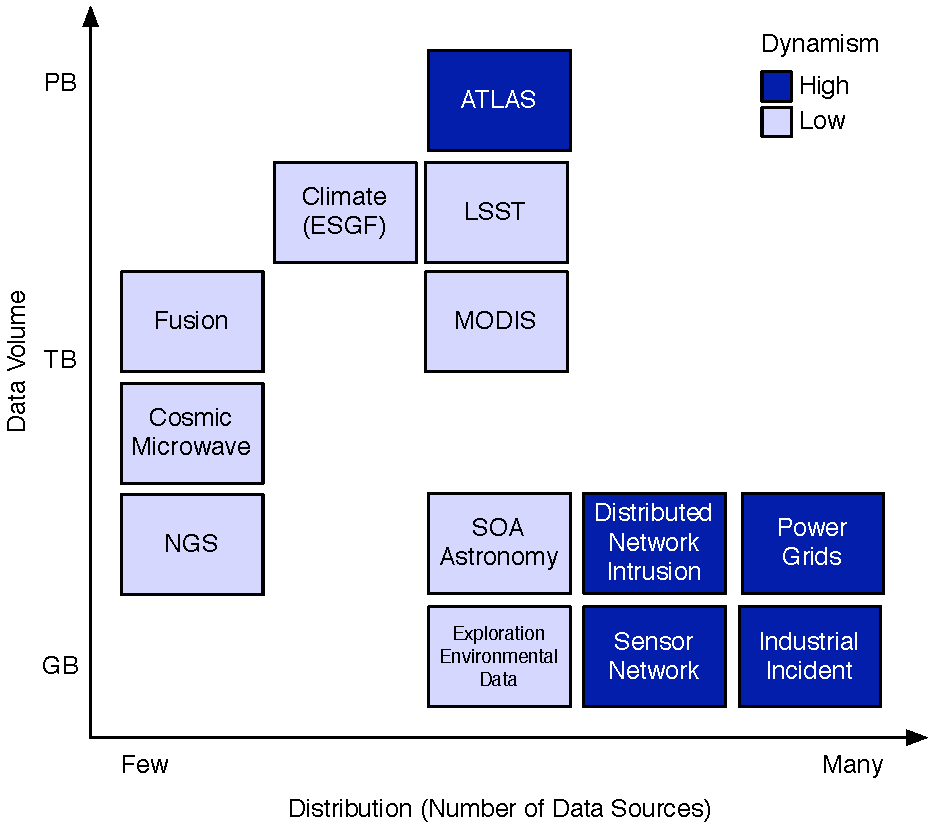
\includegraphics[width=.7\textwidth]{figures/application.pdf}
                \caption{The distribution, dynamism, data volume
                  characteristics of the surveyed D3 applications. The
                  clustering of applications with high dynamism in the
                  bottom right hand corner indicates a similar
                  structure amongst these applications, namely
                  multiple (sensor-based) sources of data
                  generation with temporal variation in data
                  generation. Although we do not explicitly
                  color/shade traditional and infrastructural
                  applications, it is worth mentioning that there is
                  no correlation between application type and any of
                  the three ``D''s; we attribute this to a strong
                  dependence of degree-of-distribution infrastructure
                  available for both types of applications.
                  \label{fig:figures_application}}
\end{figure}

% \alnote{Think about how we can add a infrastructure dimension to this
%   figure.} \jhanote{As AL and I discussed on a call, in addition to
%   AL's suggestion, we need to also use this figure to integrate
%   section 2-4.} \jhanote{Also, how would we provide intuitive
%   explanation of high versus low dynamism?}  \jhanote{not to endlessly
%   quibble, but shouldn't ATLAS be more to the right (and higher
%   dynamism?) and NGS more the left?}


%\jhanote{the following does not make sense to
%  me..}  Additional temporal aspects pertain to the stage(s) of an
%application in which data can be distributed.

% Because application stages often have a distribution that makes sense to that
% stage, and because that distribution may not be appropriate for other
% phases, applications must either use one particular distribution that may not
% work well in all phases or transform the data on input to some stages. 

% Applications must either use one particular distribution, or transform data on
% input to some stages. In particular, 

% Infrastructural applications require a specific distribution for the data
% storage, and thus  stages that read and process the data will need to make
% this choice.  As seen, 

{\it Data topology} can be used to identify the flow of data through the
application, with nodes representing execution units and edges representing
communication features.  One aspect of managing data topology is ``data
planning," which refers to how the data is coordinated from ingest through
analysis to output. In all cases, there is a coordination of the data with code
used to analyze or transform it. In some cases these form clear, integrated
stages where data flows from one to another. In others the way that data enters
and flows through the application is more loosely defined and the execution of
code is independent. Some examples include the ATLAS experiments, which have a
single point of primary data generation which fans out to multiple analysis
sites followed by mass exchange of derived data, and sensor grids, which have
multiple sources of data generation collected to a single point of analysis
followed by constrained point of reuse.

% We observe that pipelines provide a useful abstraction to represent
% the application stages identified in
% \figurename~\ref{fig:figures_application-stages}.  Many workflow tools
% also enable simple data capture and processing pipelines to be
% defined, where each pipeline stage may range from a complete
% application to a subroutine in Matlab (for instance).  It is useful to
% note that pipelines may also be dynamically constructed and adapted
% using context and monitoring information, as undertaken in the
% Industrial Incident Notification and Response application studied in
% this paper. In this instance, the actual pipeline stage to be invoked
% is triggered by the availability of particular types of data, a
% feature also relevant in the Power Grids application.  However, it is
% useful to note that different stages of the pipeline receive different
% emphases in different applications.

Some applications must collect and store all incoming data, with only minor
pre-processing to clean the data ahead of the main processing. For others, a
major constraint is to reduce the incoming data stream as quickly as possible,
perhaps discarding a large fraction of the data before any processing occurs.

Although dynamic and distributed properties have been characterized
separately, it is important to remember, as the above patterns
indicate, that distribution and dynamism become increasingly
correlated at extreme scales.  For example, applications that run on
distributed infrastructures are often also highly dynamic and vice
versa.




% \jhanote{There is a problem here. I am not saying the following is
%   incorrect, but ultimately coordination mechanisms are being touted
%   as a way to support dynamic behaviour if not respond to dynamic
%   behaviour. However in Section 3, this is not even hinted at. Needs
%   fixing IMO. The following should be trivial: we need to relate which
%   dynamic behaviour -- infrastructure, application or data dynamism,
%   is coordination influencing?}


% \jhanote{this is the first occurence of topology. can this be removed?
%   SJ to reduce last 2 paragraphs into a few sentences}

% \rananote{Update description of data topology -- relate it to
%   pipelines and workflows mentioned earlier in the paper. Avoid
%   confusion in terminology}.  \jhanote{Also can this be related to
%   section 5.2?}



% Nonetheless, understanding the trend of say, $\beta_1$ as the degree
% of distribution changes can be insightful.

\subsubsection{Understanding Distributed Dynamic Applications: }
\label{sec:quantifyingdistapps}

In \S\ref{sec:distdyndata} we characterized dynamic and distributed
properties of the D3 Science applications. Our analysis was
qualitative by necessity, due to the fact that approaches to quantify
dynamism and distributed properties were often intimately tied to
application/scenario definition and specific usage modes.
Notwithstanding, to quantify better dynamic properties of an
application, we believe a term analogous to the use of Amdahl's
number~\cite{10.1109/ICDE.2000.839382} could be used to characterize `static'
data-intensive applications and systems:

\begin{itemize}
\item[] $\alpha$ = Num. of Compute Operations / Amount of Data
  (Consumed, Generated or Transformed)
\end{itemize}

Note that this term is scale-invariant, i.e., a value of 1 could
correspond to very small or very large values of both numerator and
denominator, and that it does not capture the time scales over
which data changes. 

% However, we believe it captures most of the non-temporal {\it dynamic}
% properties.

% \jhanote{we might consider removing the definitions. More text about
%   what is $\alpha$ and $\beta$ and say it is early work..}

% defined above for dynamic characteristics,

Similarly, another term can be used to quantify the
``scale'' of distribution, namely the degree of distribution as a
function of the amount of data transferred, where the degree of
distribution can be defined as the number of distinct data locations:

\begin{itemize}
\item[] $\beta$ = Amount of Data Transferred / Degree of
  Distribution
% \item[] $\beta_2$ = Number of Compute Operations / Degree of
%   Distribution
\end{itemize}

%Specifically, we propose $\beta$ as a ratio of the amount of data
%transferred to the number of distinct sites (i.e., degree) that it was
%distributed over.


% either the computation involved or For a given application, the
% degree of distribution is often dependent or correlated with the
% total number of computational operations involved or the amount of
% data transferred, e.g., for small computational operations or
% data-volumes there is typically a limited amount of flexibility in
% distribution before the overhead of distribution (either source or
% destination) dominates.


% and $\beta_2$ as a ratio of the number of compute operations to the
% degree of distribution; as can be expected, for low amounts of
% compute units the extent to which the tasks can be distributed is
% limited, as overhead costs may dominate.



%Notwithstanding, in this subsection, we provided a framework for

It has proven difficult to provide ``global'' quantitative values of
these ratios, as often the value of the numerators is
subject to how an application/scenario is defined, even more so for a
``class of applications'' as opposed to a specific application. We
believe, nonetheless, that these measures suggest a possible way to
quantify an application's dynamism and distribution and thereby find
possible common approaches solutions.  We plan to explore this in our
future work, and also hope others will consider building on these
initial concepts.

%and thus providing well-defined numbers is difficult,

\subsubsection{Towards an Architecture for D3 Science?}

%\jhanote{Note to self: need smoothening}

An investigation of data-intensive distributed applications on production
cyberinfrastructure, leads us to believe that there are three primary
macroscopic architectures and approaches for distributed data-intensive
applications: (i) localize all data into a ``cloud'' (or a large analytical
engine) -- the paradigm adopted by several genome projects and the cancer atlas,
(ii) decompose and distribute data to an appropriate number of
computing/analytical engines as available -- the paradigm employed by particle
physics for the discovery of the Higgs Boson (similar to the application in
\S\ref{WLCGSteve}), and (iii) a hybrid of the above two paradigms, wherein data
is decomposed and committed to several infrastructure, which in turn could be a
combination of either of the first two paradigms, similar to what is done in the
Power grids application
(\S\ref{power}). %\jhanote{improve description....replace hybrid by bottom-up? }

It is obvious that the first architecture can be used for large volumes of data,
but there are self-evident limitations to the scalability or validity of this
model. How does this limitation change, qualitatively or quantitatively, if
dynamic data and/or applications are considered? This begets the question: how
fundamental an issue is {\it dynamic}?

The high-energy physics (HEP) community has self-organized towards the
second architectural approach.  Although distributed computing
infrastructures representing this approach, such as OSG and EGI, have
been successful for this community and application, broad uptake
across other application types, modes, and data volumes has not taken
place. What lessons does the HEP experience teach us for the other
communities, such as bioinformatics?  Can an infrastructure
conforming to a particular architecture and developed for a specific
application domain be generalized to another science domain, using the
same underlying macro architecture but by providing a different set of
services and specialized data cyberinfrastructure? Or is the
architecture specific to a {\it fixed} range of compute-data
characteristics? If so, what are these characteristics?


%\subsection{Observations}
%
%\katznote{some text needed here.  Note that I promoted this from 5.1.5 to 5.2, thinking that 5 might be best as discussion, observations, conclusions - how we order 5.1 and 5.2 is still a question... Maybe call this `takeaway points'?}
%
%\katznote{Omer to go through and move the text/points to either Discussion or Conclusions... This section will then empty/removed}

%\begin{itemize}

%\item In \S\ref{sec:scenarios}, we divided applications into groups:
%  traditional and infrastructural applications.  Traditional
%  applications have been built by one or more authors in order to
%  solve a particular problem or to answer a science question.
%  Infrastructural applications have been built by groups or
%  communities to allow the solution of a set of problems, or to answer
%  a set of science questions.  In both cases, we can observe that the
%  same set of applications stages (as shown in
%  \figurename~\ref{fig:figures_application-stages}) can be applied,
%  with APIs defined as the inputs and outputs of those stages.  These
%  APIs are very informal and loose for the traditional applications,
%  but more fixed and conservative for the infrastructural
%  applications.  These APIs limit how new paradigms can be used for
%  the infrastructural applications, unless those paradigms happen to
%  fit the existing APIs.  Another way of saying this is that the
%  abstractions for dynamism and distribution that can be used in the
%  infrastructural applications are those abstractions that the
%  developers of the original applications were aware of at the time
%  the infrastructural applications were defined.  This leads to a
%  possible mismatch, where computer scientists have new ideas that
%  could be applied to the class of problems that an infrastructural
%  application was designed to solve, but that the infrastructural
%  application doesn't allow, due to the fixed APIs.  Workflow systems
%  are a possible way of solving this problem, as they are often
%  sufficiently domain-independent that there does not seem to be a tie
%  of a particular system to a particular infrastructural application.

%\item There exist patterns in the described applications; however,
%  implementation and deployment specific details often mask these
%  patterns.  For example, applications often differ in the way they
%  handle distribution and dynamism, such as managing such as
%  data/compute localities. This makes it difficult to support patterns
%  of distribution and dynamism in a general-purpose fashion, for
%  anything but the simplest patterns.
%
%\item It is useful to observe that pipelines provide a useful
%  abstraction to represent the application stages identified in
%  \figurename~\ref{fig:figures_application-stages}.  Many workflow
%  tools also enable simple data capture and processing pipelines to be
%  defined, where each pipeline stage may range from a complete
%  application to a subroutine in Matlab (for instance).  It is useful
%  to note that pipelines may also be dynamically constructed and
%  adapted using context and monitoring information, as undertaken in
%  the Industrial Incident Notification and Response application
%  studied in this paper. In this instance, the actual pipeline stage
%  to be invoked is triggered by the availability of particular types
%  of data, a feature also relevant in the Power Grids application.
%  However, it is useful to note that different stages of the pipeline
%  receive different emphases in different applications. Some
%  applications must collect and store all incoming data, with only
%  minor pre-processing to clean the data ahead of the main
%  processing. For others, a major constraint is to reduce the incoming
%  data stream as quickly as possible, perhaps discarding a large
%  fraction of the data before any processing occurs. Reuse of pipeline
%  stages across different applications must therefore be undertaken
%  with care.

  % Managing and coordinating the behavior of pipeline execution, for
  % supporting both file-based and streaming data, has been
  % extensively studied in computer science (supporting synchronous
  % (blocking), asynchronous, concurrent, threading semantics, for
  % instance).

%\item

%\jhanote{mismatch between abstraction levels, reference SAGA
%  paper ``leaky abstractions''} \katznote{Shantenu to incorporate this
%  into the leaky abstraction stuff above} \katznote{A possible problem is
%  that distributed systems (infrastructures and perhaps applications)
%  are so different from each other that there is no common system
%  abstraction that is both general enough to work on all of them and
%  specific enough to be useful on any of them.}

%\item The trend toward more unstructured and more dynamic data sources lead to
%higher demands on data processing infrastructure.
%  provide simple abstractions or frameworks to
%  Higher-level abstraction need to provide sufficient level of control
%  of infrastructure trade-offs (such as data/compute localities),
%  while hiding a lot of the complexities (e.g.., the management of
%  replicas).\jhanote{andre to try to link back to section 4 and
%    elaborate}

% This indicates the difficulty of
%  using existing abstractions and infrastructures.


%\jhanote{Worth having in this section. Needs integration}

% \item Often the coupling between the various components/services that
%   are part of the workflow can differ -- ranging from hardwired
%   interactions between components to those that can be defined and
%   modified by an application developer. We can therefore distinguish
%   between workflows that are embedded within an application, to those
%   that are explicitly defined using a composition tool (such as
%   Taverna, Triana, Kepler, etc). Workflow systems often utilize a
%   variety of abstractions related to: (i) mapping of
%   services/components to computational/data resources; (ii) data
%   movement/migration; and (iii) coordination between various
%   components.  And,
%   in many cases, they do not appear to be widely used where we might
%   think they would be, perhaps due to lack of publicity, steep
%   learning curves, or other issues.

%\end{itemize}

%\subsection{Points + Hypotheses}

\subsection{Conclusions}
\label{sec:conclusion}

The growth in data volumes and its importance is having profound implications on
the way applications are designed and the way we develop infrastructure and
provision associated services.  Many fields, such as biology, that until
recently were not characterized by their intensive use of data are rapidly
becoming data-driven.

Associated with the growth in data volumes are increasing levels of dynamism and
distribution; sometimes distribution is logical, but sometimes the data is
physically distributed for reasons of performance or convenience. At large
scales, dynamism becomes intrinsic to the application and infrastructure;
sometimes it occurs because of changing experimental or analytic conditions,
sometimes due to the availability of infrastructure and resources.

An important motivation for this work is to capture the state of the art in the
design and development of distributed dynamic applications and the associated
infrastructure currently used for their execution. We have aimed to try to
discern common approaches and challenges, and to identify any obvious gaps (or
opportunities). Using a common vocabulary and terminology to describe otherwise
distinct and unrelated applications allows potential application
users\slash developers to benefit from the insights that a common analytical framework
provides. For example, seeing how applications with similar patterns (e.g.,
pipelines) have addressed issues of dynamism and distribution enables common
solutions and facilitates the emergence of best practices even in the absence of
formal methods.  Similarly, our analysis sends a useful message to domain and
application scientists that the challenges and barriers they face are not unique
even if current solutions require a level of customization.  In this paper, we
have identified many different applications characteristics, programming
systems, and infrastructure techniques that either support dynamic data or
produce it.

% For example, there is a lifecycle to data that has often been ignored until
% recently: the decreasing cost of storage has made it attractive to archive
% \emph{everything}, just in case it becomes useful. This approach is becoming
% untenable in many areas: some datasets are simply too big to archive, and so
% must be summarized and their raw form discarded (possibly in real time). Others
% are easier to regenerate than to store.  Still others are too transient to
% justify their storage, and may in aggregate be too big to store even when being
% small individually.  Additionally, it is useful to observe that the trend toward
% more unstructured and more dynamic data sources lead to higher demands on data
% processing infrastructure~\cite{snia_2012}. Any data science architecture needs
% to explicitly recognize, capture, and manage the lifecycle requirements of
% different datasets, within the constraints of available time and storage.


% Consistent with experience in other related fields, there seems no reason to
% expect that these approaches and techniques will disappear in the near
% future. While a convergence in approaches and techniques might be expected, this
% has proved to be elusive; there remains a diversity in the design,
% implementation, and execution of scientific codes.  It may even be argued that
% it is premature to have convergence; after all, D3 Science is still an emerging
% domain.

% From the previous discussion we can draw out some conclusions about the trends
% within dynamic, distributed, data-intensive science. For instance, 

In \S\ref{sec:scenarios}, we divided applications into groups: traditional and
infrastructural applications.  Traditional applications have been built by one
or more authors in order to solve a particular problem or to answer a science
question.  Infrastructural applications have been built by groups or communities
to allow the solution of a set of problems, or to answer a set of science
questions. All applications in general, but infrastructural applications in
particular cannot be developed in vacuum; they must be executed on shared
infrastructure, and are thus sensitive to the external tools and services, as
well as their provisioning as software-systems.

As part of this survey, we observe that there exist patterns in the described
applications; however, implementation and deployment specific details can often
mask these patterns.  For example, applications often differ in the way they
handle distribution and dynamism, such as managing such as data/compute
localities. This makes it difficult to support patterns of distribution and
dynamism in a general-purpose fashion, for anything but the simplest patterns.

% In both cases, we can observe that the same set of applications stages (as shown
% in \figurename~\ref{fig:figures_application-stages}) can be applied, with APIs
% defined as the inputs and outputs of those stages.  These APIs are very informal
% and loose for the traditional applications, but more fixed and conservative for
% the infrastructural applications. These APIs limit how new application
% paradigms can be introduced for the infrastructural applications, unless those
% paradigms happen to fit the existing APIs.  Another way of saying this is that
% the abstractions for dynamism and distribution that can be used in the
% infrastructural applications are those abstractions that the developers of the
% original applications were aware of at the time the infrastructural applications
% were defined.  This leads to a possible mismatch, where computer scientists have
% new ideas that could be applied to the class of problems that an infrastructural
% application was designed to solve, but that the infrastructural application
% doesn't allow, due to the fixed APIs.  New tools may be developed to address a
% narrow set of features while ignoring the larger set of problems that prevented
% earlier tools from being used.  These tools then may be used by new applications
% as those applications are developed; however, they are unlikely be used by the
% existing applications they were meant to help.


% constraints on the applications lead to new tools that are or could be developed
% not being able to be applied in practice.

% For example, while workflow systems are often sufficiently domain-independent
% that there does not seem to be a tie of a particular system to a particular
% infrastructural application, there are a very large number of workflow systems
% that exist, and it is common in the authors' experience to hear about new ones
% being developed from scratch because ``the ones that exist don't quite do what
% is needed for my application or system.''

%\katznote{previous 2 paragraphs to be re-read.  Old comments about them
%are available as commented out comments.}
%\jhanote{Irrespective, I find this past paragraph
%  somewhat speculative. And I don't see the point of it? WHat is the
%  latter half trying to say: there are problems with APIs and
%  interfaces of 3D applications and systems?} \katznote{It's saying
%  that applications aren't developed in a vacuum, particularly
%  infrastructural applications, and that the constraints on the
%  applications leads to new tools that are or could be developed not
%  being able to be applied in practice.  In some ways, it's a call for
%  an application abstraction or middleware, between the applications
%  and the `infrastructure' as defined in \S4, much as perhaps AIMES is
%  trying to build}\jhanote{Dan, I find your explanatory note more
%  convincing than the sentence on workflow systems! Also there is no
%  mention of middleware as the ``impedance mismatch lowering layer''
%  in the above. I propose we rewrite the sentence starting, ``Workflow
%  systems are a possible way..} \katznote{ok, I used some of my text
%  and turned around the sentence from Omer's optimistic view to
%  my more pessimistic view.  If others disagree, we can change it back
%  or compromise.}


% In \S\ref{sec:quantifyingdistapps} we have attempted to initiate a discussion in
% this context however by considering two ratios to relate data volume and
% distribution with compute operations performed by an application. We believe
% determining values for these parameters would provide a useful starting point
% for comparing infrastructure requirements of data-intensive applications and
% systems.

%\jhanote{I transposed the last two paragraphs}






% \item Workflows seem to be a natural idea for expressing both
%   traditional and infrastructural applications, and indeed, there are
%   a number of workflow tools that are used in both cases.  It might
%   also seem that an infrastructural application would have a specific
%   workflow system that is in common use, since different
%   developers/users are all doing similar computational work, but this
%   does not appear to be true, at least in the applications we studied.

  % \katznote{I would like to say that specific workflow systems are
  %   successful when embedded inside traditional applications,
  %   because they then become part of the application, but I am not
  %   sure I have a good example here from \S\ref{sec:scenarios}.
  %   Does anyone else?}

% \begin{itemize}

% \item \jhanote{Is the following observation, hypothesis and how do we
%   link them?} \katznote{Can we say something about applications that
%   deal with files vs those that deal with streams (stream-based are:
%   PowerGrid, Fusion, Incident Response, network monitoring) PowerGrid
%   and Incident apps have centralized stream processing;} Fusion and
%   network have distributed stream processing.  Not sure what to say
%   here.  Maybe this point isn't a point... \jhanote{Look at tables
%     \ref{tab:app_distributed_processing} and
%     \ref{table:progSystems}. From these tables can we say something
%     about ``common'' ways of say distribution for ``stream based
%     applications''} \jhanote{analogy with abstractions for workflows:
%     num. of data elements, num of streams, num. dynamic resources}

% \end{itemize}



\section*{Acknowledgements}
This work was sponsored by NSF OCI-1059635 and made possible by the UK e-Science
Institute Research Theme on Dynamic Distributed Data-Intensive Programming
Abstractions and Systems. We thank Simon Dobson, Jon Weissman and Jon Blower for
useful initial discussions, as well as 3DPAS workshop attendees. Discussions of
the selected applications benefited from the generous help of Adam Barker, Jon
Blower, Julian Borrill, Silvia Delgado Olabarriaga, Steve Fisher, Keith Jackson,
Scott Klasky, Bob Mann, Don Middleton, Kees Nieuwenhuis, Manish Parashar,
Stephen Pascoe, and Jon Weissman, though any errors are the responsibility of
the authors.  Some of the work by Katz was supported by the National Science
Foundation while working at the Foundation; any opinion, finding, and
conclusions or recommendations expressed in this material are those of the
author(s) and do not necessarily reflect the views of the National Science
Foundation.

\bibliographystyle{unsrt}
\bibliography{3dpas}

\newpage
\appendix
\section*{Appendix: Methodology}

This paper originated in work at the UK e-Science Institute (eSI) at
the University of Edinburgh, in a research theme examining Dynamic
Distributed Data-intensive Programming Abstractions and Systems,
called 3DPAS~\cite{3dpas-theme}.  The description of
this theme's work was:

\begin{quote}
Many problems at the forefront of science, engineering, medicine, and the social sciences, are increasingly complex and interdisciplinary due to the plethora of data sources and computational methods available today. A common feature across many of these problem domains is the amount and diversity of data and computation that must be integrated to yield insights.

For many complex data-intensive applications, moving the data may have restrictions. Increasingly important type of data-intensive applications are data-driven applications. For example, data is increasingly large-scale, distributed arising from sensors, scientific instruments \& simulations. Such data-driven applications will involve computational activities triggered as a consequence of independent data creation; thus it is imperative for an application to be able to respond to unplanned changes in data load or content. Understanding how to support dynamic computations is a fundamental, but currently a critical missing element in data-intensive computing.

The 3DPAS theme seeks to understand the landscape of dynamic, distributed, data-intensive computing: the programming models and abstractions, the run-time and middleware services, and the computational infrastructure. It will analyze existing tools and services, identify missing pieces and new abstractions, and propose practical solutions and best practices.
\end{quote}

The theme held three workshops, and in each, application scientists and
computing technologists were invited to give presentations on their work, and
then to be involved in discussions to organize and understand the presented
materials.  Between the workshops, the theme organizers also drafted outlines of
a report that was a predecessor of this paper, for discussion in the next
workshop.  Overall, there were about 50 workshop attendees.

In order to select applications and gather information about
them, during the various workshop discussions, when an
application that ``felt'' new was mentioned, we asked the person who
mentioned it to provide a written set of answers to the following questions about the
application:

\begin{enumerate}
\item What is the purpose of the application?
\item How is the application used to do this?
\item What infrastructure is used? (including compute, data, network, instruments, etc.)
\item What dynamic data is used in the application?
\begin{enumerate}
\item What are the types of data,
\item What is the size of the data set(s)?
\end{enumerate}
\item How does the application get the data?
\item What are the time (or quality) constraints on the application?
\item How much diverse data integration is involved?
\item How diverse is the data?
\item Please feel free to also talk about the current state of the
application, if it exists today, and any specific gaps that you know
need to be overcome.
\end{enumerate}

We then used the text of these answers to describe each of the applications (in \S\ref{sec:scenarios}) in terms of:

\begin{itemize}
\item What does the application do? What problem does it solve?
\item How does it do it? How does the application run?  What infrastructure does it need/use?
\item What are the big data aspects of the application?
\item What are the distributed aspects of the application?
\item What are the dynamic aspects  of the application?
\item What else is important about the application?  What does it do well?  Poorly? How was the app written? What tools does it use?
\end{itemize}

After the workshops, the theme organizers and a set of attendees who
were interested in participating started discussing how to organize
and analyze the applications and the technologies, including
infrastructure, programming systems and abstractions.  These
participants are the current authors of this paper, and this paper is
the result of that process.

As part of the theme, two 3DPAS workshops~\cite{3dapas,D3-escience}
were organized at major conferences: HPDC 2011 and IEEE eScience 2011.
These workshops had both peer-reviewed and invited papers.

A combination of invitation-only focused discussion meetings and
broader community engagement events were used to ensure that the
applications surveyed and ideas captured in this paper are
representative of current community thinking as well as of
intellectual relevance.


\end{document}

{\em Workflow} systems have already received significant attention in
the collaborative e-Science domain.  Such systems provide a useful
means to aggregate capability and subsequently deploy the resulting
workflow over multiple, distributed resources. Workflows can be
``abstract'', i.e., only the connectivity graph is identified but is
not bound to particular executables and particular resources, or
``concrete'', i.e., the executable components are identified along
with their execution environment. Generally, an abstract workflow
needs to be mapped to a concrete workflow graph to enable
execution. This may be achieved dynamically using a variety of
different user-specified criteria, ranging from cost of execution
(such as with the availability of remotely accessed resources from
Amazon.com~\cite{berriman11}), Quality of Service, etc. This mapping
can also be adaptive, especially if each concrete workflow is
dynamically composed based on event triggers from the execution
environment or constraints identified by a user. We may therefore
identify a range of possibilities:

\begin{itemize}

\item An abstract workflow graph is statically defined and mapped to a known resource/infrastructure pool.

\item An abstract workflow graph is dynamically mapped to an infrastructure based on user-specified constraints (related to cost of access, Quality of Service, etc.)

\item An abstract workflow graph is dynamically enacted over a varying infrastructure pool (often making use of an external resource management system.)

\item An abstract workflow graph is used to dynamically compose a concrete workflow using techniques from AI planning and model checking.

\end{itemize}

Workflow tools such as Taverna~\cite{Taverna}, Kepler~\cite{Kepler},
Trident~\cite{Trident} and others~\cite{iantaylorsbook} \jhanote{Are
  any of these used by applications? If not I propose they not be
  mentioned} enable reusable code for scientific analysis by
expressing it as an explicit dataflow or control flow composition of
components, each serving a dedicated function. This has simplified the
development and the maintenance of complex codes, both by allowing
common component re-use and by highlighting the structure of the
processing pipeline. Workflow tools therefore provide both
infrastructure for supporting the construction and enactment/execution
of scientific applications and components that be used alongside
application specific infrastructure. The granularity of a workflow
tool can therefore range from simple components to complete
infrastructures (i.e. enabling integration of other components and
supporting their enactment/execution).

